% Appendix-scoped float tuning: from here on, a two-column [t] float (no "!")
% may claim at most 60% of a page top.  This splits the three COLOSSEUM
% per-task tables onto consecutive text pages (one table + discussion each)
% instead of stacking two of them over a thin strip of text.  Floats marked
% [!t] (the two real-robot tables) and [p] (the per-task gallery) are exempt.
% The main body is built before this point and is unaffected.
\renewcommand{\dbltopfraction}{0.6}

\subsection{Per-Task Results on COLOSSEUM}
\label{app:colosseum_results}

COLOSSEUM and GemBench, covered here and in
Appendix~\ref{app:gembench_results}, hold the training data fixed and
shift the test environment away from it in appearance, objects, and
instructions.
Because both suites probe per-frame perception rather than history, the
base policy \method\ carries the comparison against prior work;
\memmethod\ is reported alongside it to verify that the memory
extension preserves this robustness.

On COLOSSEUM~\cite{pumacay2024colosseum} (settings and protocol in
Appendix~\ref{app:eval_protocol}, perturbations visualized in
Fig.~\ref{fig:vis_colosseum}), we compare against
R3M-MLP~\cite{nair2022r3m} and MVP-MLP~\cite{xiao2022masked}, which
pair pre-trained 2D encoders with MLP action heads, and against the 3D
policies PerAct~\cite{shridhar2023perceiver}, RVT~\cite{goyal2023rvt},
and RVT-2~\cite{goyal2024rvt}.

Beyond the averages reported in Sec.~\ref{sec:exp:additional}, \method\
ranks best among prior methods in 13 of the 14 settings
(Table~\ref{tab:colosseum}), and how that margin is distributed
supports the alignment argument: it is widest under appearance-level
shifts, with a lead of 11 to 15 points on table texture, table color,
light color, and receptacle texture, which is exactly the nuisance
variation a VLM's 2D pre-training has seen in abundance and a policy
trained from scratch has not.
The one setting in which \method\ trails is \emph{Distractor}, at
51.8\% against 60.8\% for RVT-2.
\memmethod\ improves markedly on precisely the two settings that are
hardest for \method, reaching 38.9\% against 18.7\% under \emph{All
Perturbations} and 61.6\% against 51.8\% under \emph{Distractor}, and
between them the two variants rank first in every one of the 14
settings.
Tables~\ref{tab:results_bridgevla},
\ref{tab:results_bridgevla_plus}, and~\ref{tab:results_rvt2} break the
comparison down to the task level.

\begin{table*}[t]
\centering
\caption{\textbf{Per-Task Results of \method\ on COLOSSEUM.}
Success rates (\%) under each COLOSSEUM
perturbation~\cite{pumacay2024colosseum}, mean$\pm$variance over three
evaluation repetitions;
% TODO(user): confirm from the eval logs whether the subscripts are std or
% variance; the source text says "variance", kept here for consistency.
``--'' marks perturbation--task combinations the benchmark does not
define.}
\label{tab:results_bridgevla}
\footnotesize
\setlength{\tabcolsep}{4pt}
% zero rule separation; \arraystretch below compensates the row height
\setlength{\aboverulesep}{0pt}
\setlength{\belowrulesep}{0pt}
\renewcommand{\arraystretch}{1.25}
\resizebox{\fitwidth}{!}{%
\begin{tabular}{l*{15}{c}}
\toprule
\textbf{Task} & \rotatebox[origin=c]{90}{\textbf{Original}} & \rotatebox[origin=c]{90}{\textbf{All Perturbations}} & \rotatebox[origin=c]{90}{\textbf{MO-COLOR}} & \rotatebox[origin=c]{90}{\textbf{RO-COLOR}} & \rotatebox[origin=c]{90}{\textbf{MO-TEXTURE}} & \rotatebox[origin=c]{90}{\textbf{RO-TEXTURE}} & \rotatebox[origin=c]{90}{\textbf{MO-SIZE}} & \rotatebox[origin=c]{90}{\textbf{RO-SIZE}} & \rotatebox[origin=c]{90}{\textbf{Light Color}} & \rotatebox[origin=c]{90}{\textbf{Table Color}} & \rotatebox[origin=c]{90}{\textbf{Table Texture}} & \rotatebox[origin=c]{90}{\textbf{Distractor}} & \rotatebox[origin=c]{90}{\textbf{Background Texture}} & \rotatebox[origin=c]{90}{\textbf{RLBench}} & \rotatebox[origin=c]{90}{\textbf{Camera Pose}} \\
\midrule
basketball\_in\_hoop & 100.0$\pm$0.0 & 4.0$\pm$3.3 & 94.7$\pm$1.9 & 96.0$\pm$0.0 & 84.0$\pm$5.7 & -- & 100.0$\pm$0.0 & 68.0$\pm$0.0 & 100.0$\pm$0.0 & 100.0$\pm$0.0 & 100.0$\pm$0.0 & 37.3$\pm$1.9 & 100.0$\pm$0.0 & 100.0$\pm$0.0 & 100.0$\pm$0.0 \\
close\_box & 100.0$\pm$0.0 & 72.0$\pm$0.0 & 94.7$\pm$1.9 & -- & -- & -- & 93.3$\pm$1.9 & -- & 100.0$\pm$0.0 & 100.0$\pm$0.0 & 98.7$\pm$1.9 & 98.7$\pm$1.9 & 100.0$\pm$0.0 & 97.3$\pm$1.9 & 100.0$\pm$0.0 \\
close\_laptop\_lid & 100.0$\pm$0.0 & 11.1$\pm$15.7 & 82.7$\pm$3.8 & -- & -- & -- & 67.9$\pm$14.6 & -- & 89.3$\pm$8.2 & 92.0$\pm$0.0 & 97.3$\pm$3.8 & 82.7$\pm$6.8 & 96.0$\pm$3.3 & 100.0$\pm$0.0 & 96.0$\pm$0.0 \\
empty\_dishwasher & 0.0$\pm$0.0 & 0.0$\pm$0.0 & 1.3$\pm$1.9 & 1.3$\pm$1.9 & -- & 1.3$\pm$1.9 & 4.0$\pm$3.3 & 0.0$\pm$0.0 & 0.0$\pm$0.0 & 0.0$\pm$0.0 & 0.0$\pm$0.0 & 0.0$\pm$0.0 & 1.3$\pm$1.9 & 1.3$\pm$1.9 & 0.0$\pm$0.0 \\
get\_ice\_from\_fridge & 94.7$\pm$1.9 & 5.3$\pm$1.9 & 86.7$\pm$1.9 & 90.7$\pm$7.5 & 90.7$\pm$5.0 & -- & 84.0$\pm$3.3 & 73.3$\pm$1.9 & 96.0$\pm$3.3 & 98.7$\pm$1.9 & 89.3$\pm$7.5 & 56.0$\pm$8.6 & 94.7$\pm$1.9 & 96.0$\pm$3.3 & 98.7$\pm$1.9 \\
hockey & 57.3$\pm$5.0 & 9.3$\pm$3.8 & 44.0$\pm$6.5 & 50.7$\pm$8.2 & -- & 50.7$\pm$13.2 & 46.7$\pm$8.2 & 65.3$\pm$5.0 & 45.3$\pm$1.9 & 64.0$\pm$8.6 & 53.3$\pm$1.9 & 20.0$\pm$3.3 & 56.0$\pm$5.7 & 49.3$\pm$5.0 & 50.7$\pm$5.0 \\
insert\_onto\_square\_peg & 93.3$\pm$3.8 & 23.3$\pm$2.4 & 52.0$\pm$3.3 & 94.7$\pm$1.9 & -- & 76.0$\pm$8.6 & 85.3$\pm$3.8 & 70.7$\pm$3.8 & 84.0$\pm$0.0 & 88.0$\pm$3.3 & 88.0$\pm$3.3 & 44.0$\pm$11.8 & 86.7$\pm$1.9 & 77.3$\pm$5.0 & 96.0$\pm$0.0 \\
meat\_on\_grill & 96.0$\pm$0.0 & 9.3$\pm$1.9 & 32.0$\pm$0.0 & 88.0$\pm$5.7 & -- & -- & 100.0$\pm$0.0 & -- & 100.0$\pm$0.0 & 92.0$\pm$6.5 & 90.7$\pm$1.9 & 98.7$\pm$1.9 & 97.3$\pm$1.9 & 100.0$\pm$0.0 & 100.0$\pm$0.0 \\
move\_hanger & 37.3$\pm$3.8 & 2.7$\pm$3.8 & 26.7$\pm$3.8 & 46.7$\pm$3.8 & -- & -- & -- & -- & 52.0$\pm$0.0 & 84.0$\pm$0.0 & 52.0$\pm$5.7 & 52.0$\pm$5.7 & 33.3$\pm$5.0 & 42.7$\pm$1.9 & 24.0$\pm$0.0 \\
open\_drawer & 96.0$\pm$0.0 & 60.0$\pm$3.3 & 97.3$\pm$1.9 & -- & -- & -- & 90.7$\pm$1.9 & -- & 88.0$\pm$3.3 & 93.3$\pm$1.9 & 100.0$\pm$0.0 & 90.7$\pm$1.9 & 100.0$\pm$0.0 & 94.7$\pm$1.9 & 96.0$\pm$0.0 \\
place\_wine\_at\_rack\_location & 88.0$\pm$5.7 & 17.3$\pm$13.6 & 82.7$\pm$5.0 & 89.3$\pm$7.5 & -- & 92.0$\pm$6.5 & 93.3$\pm$3.8 & 90.7$\pm$3.8 & 90.7$\pm$5.0 & 97.3$\pm$1.9 & 88.0$\pm$3.3 & 74.7$\pm$3.8 & 90.7$\pm$6.8 & 92.0$\pm$3.3 & 92.0$\pm$8.6 \\
put\_money\_in\_safe & 94.7$\pm$1.9 & 6.7$\pm$5.0 & 78.7$\pm$1.9 & 74.7$\pm$1.9 & 81.3$\pm$6.8 & 89.3$\pm$5.0 & 92.0$\pm$3.3 & -- & 37.3$\pm$12.4 & 84.0$\pm$3.3 & 84.0$\pm$3.3 & 84.0$\pm$3.3 & 89.3$\pm$1.9 & 86.7$\pm$8.2 & 86.7$\pm$1.9 \\
reach\_and\_drag & 100.0$\pm$0.0 & 0.0$\pm$0.0 & 89.3$\pm$3.8 & 96.0$\pm$0.0 & 94.7$\pm$5.0 & 84.0$\pm$5.7 & 94.7$\pm$1.9 & 38.7$\pm$5.0 & 92.0$\pm$3.3 & 88.0$\pm$5.7 & 78.7$\pm$3.8 & 28.0$\pm$8.6 & 100.0$\pm$0.0 & 100.0$\pm$0.0 & 94.7$\pm$3.8 \\
scoop\_with\_spatula & 96.0$\pm$3.3 & 6.7$\pm$1.9 & 94.7$\pm$1.9 & 93.3$\pm$1.9 & 85.3$\pm$3.8 & 85.3$\pm$3.8 & 78.7$\pm$3.8 & 86.7$\pm$5.0 & 90.7$\pm$1.9 & 88.0$\pm$6.5 & 77.3$\pm$1.9 & 20.0$\pm$5.7 & 90.7$\pm$6.8 & 89.3$\pm$1.9 & 93.3$\pm$1.9 \\
setup\_chess & 10.7$\pm$1.9 & 0.0$\pm$0.0 & 1.3$\pm$1.9 & 8.0$\pm$0.0 & 8.0$\pm$3.3 & -- & 13.3$\pm$1.9 & -- & 12.0$\pm$5.7 & 21.3$\pm$8.2 & 13.3$\pm$3.8 & 5.3$\pm$1.9 & 20.0$\pm$5.7 & 16.0$\pm$5.7 & 4.0$\pm$3.3 \\
slide\_block\_to\_target & 100.0$\pm$0.0 & 24.0$\pm$3.3 & 74.7$\pm$1.9 & -- & 92.0$\pm$3.3 & -- & -- & -- & 100.0$\pm$0.0 & 100.0$\pm$0.0 & 98.7$\pm$1.9 & 84.0$\pm$9.8 & 100.0$\pm$0.0 & 100.0$\pm$0.0 & 100.0$\pm$0.0 \\
stack\_cups & 58.7$\pm$3.8 & 29.3$\pm$1.9 & 66.7$\pm$1.9 & -- & 50.7$\pm$1.9 & -- & 44.0$\pm$3.3 & -- & 62.7$\pm$1.9 & 64.0$\pm$3.3 & 65.3$\pm$8.2 & 26.7$\pm$7.5 & 73.3$\pm$8.2 & 64.0$\pm$14.2 & 72.0$\pm$8.6 \\
straighten\_rope & 61.3$\pm$6.8 & 8.0$\pm$5.7 & 16.0$\pm$5.7 & -- & 48.0$\pm$3.3 & -- & -- & -- & 61.3$\pm$9.4 & 65.3$\pm$1.9 & 54.7$\pm$8.2 & 37.3$\pm$5.0 & 70.7$\pm$8.2 & 66.7$\pm$7.5 & 72.0$\pm$6.5 \\
turn\_oven\_on & 93.3$\pm$1.9 & 85.3$\pm$3.8 & 94.7$\pm$3.8 & -- & -- & -- & 90.7$\pm$1.9 & -- & 93.3$\pm$3.8 & 94.7$\pm$7.5 & 96.0$\pm$3.3 & 96.0$\pm$3.3 & 96.0$\pm$0.0 & 88.0$\pm$3.3 & 100.0$\pm$0.0 \\
wipe\_desk & 0.0$\pm$0.0 & 0.0$\pm$0.0 & 0.0$\pm$0.0 & 0.0$\pm$0.0 & 0.0$\pm$0.0 & -- & 0.0$\pm$0.0 & -- & 0.0$\pm$0.0 & 0.0$\pm$0.0 & 0.0$\pm$0.0 & 0.0$\pm$0.0 & 0.0$\pm$0.0 & 0.0$\pm$0.0 & 0.0$\pm$0.0 \\
\midrule
Task Mean & 73.9$\pm$0.7 & 18.7$\pm$2.2 & 60.5$\pm$1.1 & 63.8$\pm$0.1 & 63.5$\pm$1.5 & 68.4$\pm$3.3 & 69.3$\pm$1.0 & 61.7$\pm$0.8 & 69.7$\pm$1.2 & 75.7$\pm$0.9 & 71.3$\pm$0.7 & 51.8$\pm$1.5 & 74.8$\pm$1.0 & 73.1$\pm$0.2 & 73.8$\pm$0.3 \\
\bottomrule
\end{tabular}%
}
\end{table*}

\begin{table*}[t]
\centering
\caption{\textbf{Per-Task Results of \memmethod\ on COLOSSEUM.}
Success rates (\%) under each COLOSSEUM
perturbation~\cite{pumacay2024colosseum}, mean$\pm$variance over three
evaluation repetitions,
% NOTE: subscripts computed as population std of the three runs, matching the
% convention of Table results_bridgevla (whose caption likewise says "variance").
under the identical protocol as Table~\ref{tab:results_bridgevla};
``--'' marks perturbation--task combinations the benchmark does not
define.}
\label{tab:results_bridgevla_plus}
\footnotesize
\setlength{\tabcolsep}{4pt}
% zero rule separation; \arraystretch below compensates the row height
\setlength{\aboverulesep}{0pt}
\setlength{\belowrulesep}{0pt}
\renewcommand{\arraystretch}{1.25}
\resizebox{\fitwidth}{!}{%
\begin{tabular}{l*{15}{c}}
\toprule
\textbf{Task} & \rotatebox[origin=c]{90}{\textbf{Original}} & \rotatebox[origin=c]{90}{\textbf{All Perturbations}} & \rotatebox[origin=c]{90}{\textbf{MO-COLOR}} & \rotatebox[origin=c]{90}{\textbf{RO-COLOR}} & \rotatebox[origin=c]{90}{\textbf{MO-TEXTURE}} & \rotatebox[origin=c]{90}{\textbf{RO-TEXTURE}} & \rotatebox[origin=c]{90}{\textbf{MO-SIZE}} & \rotatebox[origin=c]{90}{\textbf{RO-SIZE}} & \rotatebox[origin=c]{90}{\textbf{Light Color}} & \rotatebox[origin=c]{90}{\textbf{Table Color}} & \rotatebox[origin=c]{90}{\textbf{Table Texture}} & \rotatebox[origin=c]{90}{\textbf{Distractor}} & \rotatebox[origin=c]{90}{\textbf{Background Texture}} & \rotatebox[origin=c]{90}{\textbf{RLBench}} & \rotatebox[origin=c]{90}{\textbf{Camera Pose}} \\
\midrule
basketball\_in\_hoop & 100.0$\pm$0.0 & 41.3$\pm$3.8 & 96.0$\pm$0.0 & 100.0$\pm$0.0 & 94.7$\pm$1.9 & -- & 100.0$\pm$0.0 & 86.7$\pm$1.9 & 100.0$\pm$0.0 & 100.0$\pm$0.0 & 100.0$\pm$0.0 & 97.3$\pm$1.9 & 100.0$\pm$0.0 & 100.0$\pm$0.0 & 100.0$\pm$0.0 \\
close\_box & 93.3$\pm$1.9 & 84.0$\pm$0.0 & 94.7$\pm$1.9 & -- & -- & -- & 96.0$\pm$0.0 & -- & 96.0$\pm$3.3 & 96.0$\pm$0.0 & 97.3$\pm$1.9 & 94.7$\pm$5.0 & 98.7$\pm$1.9 & 98.7$\pm$1.9 & 96.0$\pm$0.0 \\
close\_laptop\_lid & 100.0$\pm$0.0 & 82.7$\pm$1.9 & 96.0$\pm$0.0 & -- & -- & -- & 100.0$\pm$0.0 & -- & 100.0$\pm$0.0 & 96.0$\pm$0.0 & 92.0$\pm$0.0 & 96.0$\pm$0.0 & 92.0$\pm$0.0 & 100.0$\pm$0.0 & 100.0$\pm$0.0 \\
empty\_dishwasher & 10.7$\pm$1.9 & 16.0$\pm$0.0 & 12.0$\pm$3.3 & 25.3$\pm$5.0 & -- & 20.0$\pm$5.7 & 37.3$\pm$5.0 & 20.0$\pm$8.6 & 4.0$\pm$3.3 & 10.7$\pm$1.9 & 12.0$\pm$0.0 & 14.7$\pm$1.9 & 14.7$\pm$1.9 & 6.7$\pm$5.0 & 21.3$\pm$5.0 \\
get\_ice\_from\_fridge & 96.0$\pm$3.3 & 22.7$\pm$6.8 & 88.0$\pm$0.0 & 98.7$\pm$1.9 & 93.3$\pm$1.9 & -- & 94.7$\pm$1.9 & 90.7$\pm$1.9 & 97.3$\pm$1.9 & 98.7$\pm$1.9 & 98.7$\pm$1.9 & 93.3$\pm$1.9 & 100.0$\pm$0.0 & 96.0$\pm$0.0 & 97.3$\pm$3.8 \\
hockey & 38.7$\pm$7.5 & 2.7$\pm$1.9 & 48.0$\pm$5.7 & 37.3$\pm$1.9 & -- & 26.7$\pm$5.0 & 22.7$\pm$5.0 & 28.0$\pm$3.3 & 22.7$\pm$3.8 & 37.3$\pm$6.8 & 26.7$\pm$5.0 & 16.0$\pm$0.0 & 26.7$\pm$1.9 & 29.3$\pm$1.9 & 33.3$\pm$5.0 \\
insert\_onto\_square\_peg & 24.0$\pm$6.5 & 58.7$\pm$5.0 & 18.7$\pm$8.2 & 41.3$\pm$1.9 & -- & 44.0$\pm$3.3 & 56.0$\pm$3.3 & 14.7$\pm$3.8 & 25.3$\pm$1.9 & 34.7$\pm$1.9 & 33.3$\pm$3.8 & 29.3$\pm$1.9 & 36.0$\pm$3.3 & 26.7$\pm$6.8 & 33.3$\pm$3.8 \\
meat\_on\_grill & 100.0$\pm$0.0 & 81.3$\pm$1.9 & 97.3$\pm$1.9 & 100.0$\pm$0.0 & -- & -- & 100.0$\pm$0.0 & -- & 100.0$\pm$0.0 & 100.0$\pm$0.0 & 100.0$\pm$0.0 & 100.0$\pm$0.0 & 100.0$\pm$0.0 & 100.0$\pm$0.0 & 100.0$\pm$0.0 \\
move\_hanger & 20.0$\pm$0.0 & 18.7$\pm$3.8 & 52.0$\pm$9.8 & 25.3$\pm$7.5 & -- & -- & -- & -- & 26.7$\pm$8.2 & 57.3$\pm$3.8 & 37.3$\pm$3.8 & 49.3$\pm$5.0 & 24.0$\pm$5.7 & 20.0$\pm$0.0 & 21.3$\pm$6.8 \\
open\_drawer & 100.0$\pm$0.0 & 69.3$\pm$1.9 & 100.0$\pm$0.0 & -- & -- & -- & 100.0$\pm$0.0 & -- & 100.0$\pm$0.0 & 100.0$\pm$0.0 & 100.0$\pm$0.0 & 74.7$\pm$5.0 & 100.0$\pm$0.0 & 100.0$\pm$0.0 & 100.0$\pm$0.0 \\
place\_wine\_at\_rack\_location & 96.0$\pm$3.3 & 77.3$\pm$5.0 & 98.7$\pm$1.9 & 100.0$\pm$0.0 & -- & 93.3$\pm$5.0 & 93.3$\pm$1.9 & 96.0$\pm$0.0 & 96.0$\pm$3.3 & 94.7$\pm$1.9 & 97.3$\pm$3.8 & 73.3$\pm$6.8 & 89.3$\pm$5.0 & 94.7$\pm$3.8 & 96.0$\pm$0.0 \\
put\_money\_in\_safe & 90.7$\pm$3.8 & 25.3$\pm$3.8 & 86.7$\pm$5.0 & 80.0$\pm$3.3 & 65.3$\pm$11.5 & 96.0$\pm$0.0 & 89.3$\pm$3.8 & -- & 81.3$\pm$5.0 & 86.7$\pm$1.9 & 77.3$\pm$6.8 & 78.7$\pm$5.0 & 89.3$\pm$3.8 & 78.7$\pm$3.8 & 73.3$\pm$5.0 \\
reach\_and\_drag & 86.7$\pm$6.8 & 5.3$\pm$1.9 & 85.3$\pm$5.0 & 94.7$\pm$5.0 & 82.7$\pm$3.8 & 88.0$\pm$0.0 & 92.0$\pm$3.3 & 81.3$\pm$1.9 & 86.7$\pm$5.0 & 80.0$\pm$5.7 & 86.7$\pm$1.9 & 77.3$\pm$5.0 & 93.3$\pm$1.9 & 89.3$\pm$1.9 & 76.0$\pm$5.7 \\
scoop\_with\_spatula & 93.3$\pm$1.9 & 21.3$\pm$1.9 & 93.3$\pm$1.9 & 88.0$\pm$3.3 & 93.3$\pm$1.9 & 90.7$\pm$5.0 & 78.7$\pm$1.9 & 78.7$\pm$5.0 & 88.0$\pm$6.5 & 96.0$\pm$3.3 & 90.7$\pm$1.9 & 62.7$\pm$6.8 & 92.0$\pm$3.3 & 93.3$\pm$1.9 & 89.3$\pm$1.9 \\
setup\_chess & 18.7$\pm$9.4 & 1.3$\pm$1.9 & 9.3$\pm$5.0 & 24.0$\pm$5.7 & 17.3$\pm$5.0 & -- & 25.3$\pm$5.0 & -- & 28.0$\pm$3.3 & 26.7$\pm$5.0 & 28.0$\pm$3.3 & 6.7$\pm$3.8 & 30.7$\pm$6.8 & 29.3$\pm$10.5 & 28.0$\pm$3.3 \\
slide\_block\_to\_target & 100.0$\pm$0.0 & 42.7$\pm$8.2 & 92.0$\pm$0.0 & -- & 96.0$\pm$0.0 & -- & -- & -- & 100.0$\pm$0.0 & 100.0$\pm$0.0 & 100.0$\pm$0.0 & 96.0$\pm$0.0 & 100.0$\pm$0.0 & 100.0$\pm$0.0 & 100.0$\pm$0.0 \\
stack\_cups & 41.3$\pm$5.0 & 5.3$\pm$1.9 & 36.0$\pm$5.7 & -- & 44.0$\pm$3.3 & -- & 37.3$\pm$1.9 & -- & 46.7$\pm$8.2 & 34.7$\pm$9.4 & 36.0$\pm$6.5 & 13.3$\pm$5.0 & 41.3$\pm$5.0 & 45.3$\pm$7.5 & 40.0$\pm$3.3 \\
straighten\_rope & 69.3$\pm$1.9 & 34.7$\pm$3.8 & 76.0$\pm$8.6 & -- & 70.7$\pm$6.8 & -- & -- & -- & 68.0$\pm$5.7 & 81.3$\pm$5.0 & 73.3$\pm$10.5 & 66.7$\pm$7.5 & 69.3$\pm$14.7 & 69.3$\pm$6.8 & 74.7$\pm$5.0 \\
turn\_oven\_on & 98.7$\pm$1.9 & 88.0$\pm$3.3 & 94.7$\pm$1.9 & -- & -- & -- & 93.3$\pm$1.9 & -- & 97.3$\pm$1.9 & 100.0$\pm$0.0 & 97.3$\pm$1.9 & 92.0$\pm$3.3 & 93.3$\pm$1.9 & 92.0$\pm$6.5 & 93.3$\pm$5.0 \\
wipe\_desk & 0.0$\pm$0.0 & 0.0$\pm$0.0 & 0.0$\pm$0.0 & 0.0$\pm$0.0 & 0.0$\pm$0.0 & -- & 0.0$\pm$0.0 & -- & 0.0$\pm$0.0 & 0.0$\pm$0.0 & 0.0$\pm$0.0 & 0.0$\pm$0.0 & 0.0$\pm$0.0 & 0.0$\pm$0.0 & 0.0$\pm$0.0 \\
\midrule
Task Mean & 68.9$\pm$0.5 & 38.9$\pm$0.8 & 68.7$\pm$0.7 & 62.7$\pm$0.6 & 65.7$\pm$0.4 & 65.5$\pm$1.2 & 71.5$\pm$0.3 & 62.0$\pm$0.7 & 68.2$\pm$1.0 & 71.5$\pm$0.3 & 69.2$\pm$0.7 & 61.6$\pm$0.5 & 69.5$\pm$1.2 & 68.5$\pm$0.6 & 68.7$\pm$0.7 \\
\bottomrule
\end{tabular}%
}
\end{table*}

\begin{table*}[t]
\centering
\caption{\textbf{Per-Task Results of RVT-2 on COLOSSEUM.}
Success rates (\%) of RVT-2~\cite{goyal2024rvt} under each COLOSSEUM
perturbation~\cite{pumacay2024colosseum}, trained and evaluated by us
under the protocol of Table~\ref{tab:results_bridgevla} (mean$\pm$variance
over three evaluation repetitions); ``--'' marks perturbation--task
combinations the benchmark does not define.}
\label{tab:results_rvt2}
\footnotesize
\setlength{\tabcolsep}{4pt}
% zero rule separation; \arraystretch below compensates the row height
\setlength{\aboverulesep}{0pt}
\setlength{\belowrulesep}{0pt}
\renewcommand{\arraystretch}{1.25}
\resizebox{\fitwidth}{!}{%
\begin{tabular}{l*{15}{c}}
\toprule
\textbf{Task} & \rotatebox[origin=c]{90}{\textbf{Original}} & \rotatebox[origin=c]{90}{\textbf{All Perturbations}} & \rotatebox[origin=c]{90}{\textbf{MO-COLOR}} & \rotatebox[origin=c]{90}{\textbf{RO-COLOR}} & \rotatebox[origin=c]{90}{\textbf{MO-TEXTURE}} & \rotatebox[origin=c]{90}{\textbf{RO-TEXTURE}} & \rotatebox[origin=c]{90}{\textbf{MO-SIZE}} & \rotatebox[origin=c]{90}{\textbf{RO-SIZE}} & \rotatebox[origin=c]{90}{\textbf{Light Color}} & \rotatebox[origin=c]{90}{\textbf{Table Color}} & \rotatebox[origin=c]{90}{\textbf{Table Texture}} & \rotatebox[origin=c]{90}{\textbf{Distractor}} & \rotatebox[origin=c]{90}{\textbf{Background Texture}} & \rotatebox[origin=c]{90}{\textbf{RLBench}} & \rotatebox[origin=c]{90}{\textbf{Camera Pose}} \\
\midrule
basketball\_in\_hoop & 100.0$\pm$0.0 & 10.0$\pm$2.0 & 99.0$\pm$1.7 & 94.0$\pm$2.0 & 97.0$\pm$1.7 & -- & 100.0$\pm$0.0 & 86.0$\pm$3.5 & 95.0$\pm$1.7 & 94.0$\pm$2.0 & 84.0$\pm$6.3 & 89.0$\pm$3.3 & 100.0$\pm$0.0 & 99.0$\pm$1.7 & 100.0$\pm$0.0 \\
close\_box & 93.0$\pm$4.4 & 36.0$\pm$8.5 & 70.0$\pm$6.6 & -- & -- & -- & 86.0$\pm$3.5 & -- & 99.0$\pm$1.7 & 97.0$\pm$1.7 & 91.0$\pm$4.4 & 93.0$\pm$3.3 & 97.0$\pm$1.7 & 94.0$\pm$2.0 & 99.0$\pm$1.7 \\
close\_laptop\_lid & 86.0$\pm$4.5 & 40.0$\pm$0.0 & 89.0$\pm$3.3 & -- & -- & -- & 62.0$\pm$2.0 & -- & 84.0$\pm$4.0 & 92.0$\pm$0.0 & 96.0$\pm$2.8 & 89.0$\pm$5.2 & 99.0$\pm$1.7 & 87.0$\pm$3.3 & 92.0$\pm$0.0 \\
empty\_dishwasher & 0.0$\pm$0.0 & 0.0$\pm$0.0 & 1.0$\pm$1.7 & 0.0$\pm$0.0 & -- & 0.0$\pm$0.0 & 0.0$\pm$0.0 & 0.0$\pm$0.0 & 0.0$\pm$0.0 & 0.0$\pm$0.0 & 0.0$\pm$0.0 & 0.0$\pm$0.0 & 0.0$\pm$0.0 & 0.0$\pm$0.0 & 0.0$\pm$0.0 \\
get\_ice\_from\_fridge & 95.0$\pm$1.7 & 11.0$\pm$4.4 & 88.0$\pm$5.7 & 77.0$\pm$5.2 & 89.0$\pm$1.7 & -- & 78.0$\pm$3.5 & 79.0$\pm$3.3 & 83.0$\pm$5.9 & 89.0$\pm$1.7 & 70.0$\pm$4.5 & 86.0$\pm$4.5 & 81.0$\pm$5.2 & 96.0$\pm$2.8 & 96.0$\pm$2.8 \\
hockey & 19.0$\pm$4.4 & 0.0$\pm$0.0 & 26.0$\pm$4.5 & 30.0$\pm$4.5 & -- & 40.0$\pm$4.9 & 24.0$\pm$2.8 & 13.0$\pm$3.3 & 12.0$\pm$8.5 & 15.0$\pm$3.3 & 9.0$\pm$3.3 & 10.0$\pm$6.0 & 14.0$\pm$2.0 & 17.0$\pm$3.3 & 19.0$\pm$3.3 \\
insert\_onto\_square\_peg & 31.0$\pm$3.3 & 0.0$\pm$0.0 & 13.0$\pm$1.7 & 35.0$\pm$9.5 & -- & 32.0$\pm$2.8 & 33.3$\pm$8.6 & 21.0$\pm$1.7 & 30.0$\pm$2.0 & 9.0$\pm$1.7 & 4.0$\pm$4.9 & 9.0$\pm$3.3 & 35.0$\pm$3.3 & 35.0$\pm$1.7 & 23.0$\pm$4.4 \\
meat\_on\_grill & 100.0$\pm$0.0 & 89.0$\pm$1.7 & 100.0$\pm$0.0 & 100.0$\pm$0.0 & -- & -- & 100.0$\pm$0.0 & -- & 99.0$\pm$1.7 & 98.0$\pm$2.0 & 100.0$\pm$0.0 & 99.0$\pm$1.7 & 100.0$\pm$0.0 & 100.0$\pm$0.0 & 100.0$\pm$0.0 \\
move\_hanger & 91.0$\pm$5.2 & 0.0$\pm$0.0 & 61.0$\pm$4.4 & 83.0$\pm$18.4 & -- & -- & -- & -- & 55.0$\pm$5.9 & 69.0$\pm$5.9 & 29.0$\pm$5.2 & 92.0$\pm$2.8 & 94.0$\pm$2.0 & 87.0$\pm$4.4 & 22.0$\pm$2.0 \\
open\_drawer & 99.0$\pm$1.7 & 25.0$\pm$4.4 & 63.0$\pm$4.4 & -- & -- & -- & 92.0$\pm$0.0 & -- & 88.0$\pm$0.0 & 92.0$\pm$0.0 & 99.0$\pm$1.7 & 86.0$\pm$8.2 & 100.0$\pm$0.0 & 95.0$\pm$1.7 & 95.0$\pm$1.7 \\
place\_wine\_at\_rack\_location & 96.0$\pm$4.9 & 28.0$\pm$6.3 & 74.0$\pm$4.5 & 98.0$\pm$2.0 & -- & 93.0$\pm$5.2 & 87.0$\pm$3.3 & 90.0$\pm$6.6 & 81.0$\pm$7.1 & 87.0$\pm$4.4 & 95.0$\pm$6.6 & 83.0$\pm$3.3 & 89.0$\pm$5.9 & 96.0$\pm$2.8 & 91.0$\pm$5.2 \\
put\_money\_in\_safe & 77.0$\pm$4.4 & 9.0$\pm$1.7 & 45.0$\pm$3.3 & 22.0$\pm$3.5 & 55.0$\pm$6.6 & 73.0$\pm$3.3 & 69.0$\pm$1.7 & -- & 56.0$\pm$2.8 & 70.0$\pm$4.5 & 72.0$\pm$6.3 & 82.0$\pm$6.6 & 79.0$\pm$3.3 & 77.0$\pm$8.7 & 62.0$\pm$6.0 \\
reach\_and\_drag & 86.0$\pm$6.6 & 0.0$\pm$0.0 & 72.0$\pm$5.7 & 80.0$\pm$5.7 & 60.0$\pm$6.9 & 67.0$\pm$5.9 & 87.0$\pm$6.6 & 55.0$\pm$4.4 & 68.0$\pm$2.8 & 76.0$\pm$2.8 & 71.0$\pm$5.2 & 61.0$\pm$6.6 & 88.0$\pm$2.8 & 86.0$\pm$3.5 & 81.0$\pm$5.9 \\
scoop\_with\_spatula & 89.0$\pm$5.2 & 2.0$\pm$3.5 & 75.0$\pm$4.4 & 87.0$\pm$3.3 & 84.0$\pm$4.9 & 92.0$\pm$7.5 & 94.0$\pm$4.5 & 83.0$\pm$5.9 & 54.0$\pm$2.0 & 79.0$\pm$5.2 & 74.0$\pm$6.0 & 83.0$\pm$5.9 & 92.0$\pm$2.8 & 91.0$\pm$1.7 & 89.0$\pm$4.4 \\
setup\_chess & 3.0$\pm$1.7 & 0.0$\pm$0.0 & 0.0$\pm$0.0 & 4.0$\pm$2.8 & 4.0$\pm$4.0 & -- & 17.0$\pm$7.1 & -- & 7.0$\pm$5.2 & 7.0$\pm$3.3 & 9.0$\pm$7.1 & 14.0$\pm$4.5 & 14.0$\pm$3.5 & 16.0$\pm$8.9 & 9.0$\pm$3.3 \\
slide\_block\_to\_target & 100.0$\pm$0.0 & 11.0$\pm$4.4 & 45.0$\pm$1.7 & -- & 97.0$\pm$1.7 & -- & -- & -- & 84.0$\pm$4.9 & 96.0$\pm$0.0 & 83.0$\pm$5.2 & 82.0$\pm$8.7 & 100.0$\pm$0.0 & 100.0$\pm$0.0 & 100.0$\pm$0.0 \\
stack\_cups & 35.0$\pm$5.2 & 0.0$\pm$0.0 & 47.0$\pm$5.9 & -- & 45.0$\pm$5.9 & -- & 23.0$\pm$4.4 & -- & 18.0$\pm$2.0 & 16.0$\pm$4.0 & 13.0$\pm$9.5 & 19.0$\pm$7.7 & 24.0$\pm$2.8 & 43.0$\pm$9.1 & 40.0$\pm$2.8 \\
straighten\_rope & 66.0$\pm$11.5 & 0.0$\pm$0.0 & 25.0$\pm$3.3 & -- & 66.0$\pm$10.0 & -- & -- & -- & 53.0$\pm$1.7 & 68.0$\pm$2.8 & 39.0$\pm$11.4 & 42.0$\pm$7.2 & 72.0$\pm$8.5 & 69.0$\pm$6.6 & 75.0$\pm$4.4 \\
turn\_oven\_on & 91.0$\pm$4.4 & 50.0$\pm$10.8 & 68.0$\pm$4.9 & -- & -- & -- & 83.0$\pm$1.7 & -- & 95.0$\pm$3.3 & 97.0$\pm$1.7 & 95.0$\pm$3.3 & 96.0$\pm$0.0 & 96.0$\pm$4.9 & 89.0$\pm$7.1 & 96.0$\pm$2.8 \\
wipe\_desk & 0.0$\pm$0.0 & 0.0$\pm$0.0 & 0.0$\pm$0.0 & 0.0$\pm$0.0 & 0.0$\pm$0.0 & -- & 0.0$\pm$0.0 & -- & 0.0$\pm$0.0 & 0.0$\pm$0.0 & 0.0$\pm$0.0 & 0.0$\pm$0.0 & 0.0$\pm$0.0 & 0.0$\pm$0.0 & 0.0$\pm$0.0 \\
\midrule
Task Mean & 67.8$\pm$1.5 & 15.6$\pm$0.8 & 53.0$\pm$0.9 & 54.6$\pm$0.6 & 59.7$\pm$0.7 & 56.7$\pm$1.4 & 60.9$\pm$0.9 & 53.4$\pm$1.5 & 58.0$\pm$1.1 & 62.6$\pm$0.9 & 56.6$\pm$0.9 & 60.8$\pm$0.5 & 68.7$\pm$1.1 & 68.8$\pm$1.3 & 64.4$\pm$0.5 \\
\bottomrule
\end{tabular}%
}
\end{table*}


\subsection{Per-Task Results on GemBench}
\label{app:gembench_results}

\begin{table}[!t]
\centering
\caption{\textbf{Results on GemBench.}
Success rates (\%) on the four generalization levels of
GemBench~\cite{garcia2024towards} (protocol in
Appendix~\ref{app:eval_protocol}).
Baselines are quoted from~\cite{garcia2024towards}, except the 3D
Diffuser Actor average, recomputed as the mean of its four levels (its
source prints 44.0).
Our rows were trained and evaluated by us on keyframes only,
without demo augmentation.
% NOTE: PolarNet L1 (77.7) and RVT-2 L1 (89.1) here follow the source's
% overall table; its per-task tables (Appendix) print 77.6 and 89.0 -- the
% rounding disagreement is inherited from the source.
Best result per column in bold.}
\label{tab:gembench}
\footnotesize
\setlength{\tabcolsep}{3pt}
% zero rule separation; \arraystretch below compensates the row height
\setlength{\aboverulesep}{0pt}
\setlength{\belowrulesep}{0pt}
\renewcommand{\arraystretch}{1.25}
\resizebox{\fitwidth}{!}{%
\begin{tabular}{lccccc}
\toprule
& \textbf{Avg.} & \textbf{L1} & \textbf{L2} & \textbf{L3} & \textbf{L4} \\
\multirow{-2}{*}{\textbf{Method}}
& \textbf{SR (\%) $\uparrow$} & \textbf{Placement} & \textbf{Rigid} & \textbf{Articulated} & \textbf{Long-Horizon} \\
\midrule
Hiveformer~\cite{guhur2023instruction} & 30.4 & 60.3$_{\pm 1.5}$ & 26.1$_{\pm 1.4}$ & 35.1$_{\pm 1.7}$ & 0.0$_{\pm 0.0}$ \\
PolarNet~\cite{chen2023polarnet}       & 38.4 & 77.7$_{\pm 0.9}$ & 37.1$_{\pm 1.4}$ & 38.5$_{\pm 1.7}$ & 0.1$_{\pm 0.2}$ \\
% NOTE: source prints Avg 44.0, but the mean of its four levels is 43.1; recomputed for arithmetic consistency.
3D Diffuser Actor~\cite{3d-da}         & 43.1 & 91.9$_{\pm 0.8}$ & 43.4$_{\pm 2.8}$ & 37.0$_{\pm 2.2}$ & 0.0$_{\pm 0.0}$ \\
RVT-2~\cite{goyal2024rvt}              & 44.0 & 89.1$_{\pm 0.8}$ & 51.0$_{\pm 2.3}$ & 36.0$_{\pm 2.2}$ & 0.0$_{\pm 0.0}$ \\
3D-LOTUS~\cite{garcia2024towards}      & 45.7 & \textbf{94.3}$_{\pm 1.4}$ & 49.9$_{\pm 2.2}$ & 38.1$_{\pm 1.1}$ & 0.3$_{\pm 0.3}$ \\
3D-LOTUS++~\cite{garcia2024towards}    & 48.0 & 68.7$_{\pm 0.6}$ & 64.5$_{\pm 0.9}$ & 41.5$_{\pm 1.8}$ & \textbf{17.4}$_{\pm 0.4}$ \\
\midrule
\textbf{\method (ours)} & 50.0 & 91.1$_{\pm 1.1}$ & 65.0$_{\pm 1.3}$ & \textbf{43.8}$_{\pm 1.2}$ & 0.0$_{\pm 0.0}$ \\
\textbf{\memmethod (ours)} & \textbf{51.1} & 88.6$_{\pm 1.1}$ & \textbf{68.9}$_{\pm 1.8}$ & 38.5$_{\pm 0.9}$ & 8.2$_{\pm 1.0}$ \\
\bottomrule
\end{tabular}%
}
\end{table}

% MemoryBench is declared here (as a single-column float, right after the
% GemBench summary) so both small tables share the page that also carries
% the COLOSSEUM RVT-2 table and the MemoryBench discussion; the per-task
% gallery tables that follow are [p] floats and pack onto pure float pages.
% Single-column float: declared right after the (also single-column) GemBench
% summary and before the [p] per-task gallery, so the in-order float queue
% places both small tables on the same text page instead of deferring this
% one past the gallery backlog.
\begin{table}[!t]
\centering
\caption{\textbf{Results on MemoryBench.}
Success rates (\%) on the three MemoryBench
tasks~\cite{fang2025sam2act}.
Baselines are quoted from~\cite{fang2025sam2act} (mean$\pm$std over
four runs; the Avg.\ deviation is the spread across the three tasks);
\method\ and \memmethod\ are mean$\pm$std over five evaluation seeds
(Appendix~\ref{app:eval_protocol}).
Best result per task in bold.}
\label{tab:memorybench}
\footnotesize
\setlength{\tabcolsep}{3.5pt}
% zero rule separation; \arraystretch below compensates the row height
\setlength{\aboverulesep}{0pt}
\setlength{\belowrulesep}{0pt}
\renewcommand{\arraystretch}{1.05}
\resizebox{\fitwidth}{!}{%
\begin{tabular}{lcccc}
\toprule
& \textbf{Avg.} & \textbf{Reopen} & \textbf{Put Block} & \textbf{Rearrange} \\
\multirow{-2}{*}{\textbf{Method}} & \textbf{SR (\%) $\uparrow$} & \textbf{Drawer} & \textbf{Back} & \textbf{Block} \\
\midrule
RVT-2~\cite{goyal2024rvt}        & 54.0$\pm$5.3  & 60.0$\pm$0.0 & 50.0$\pm$2.3  & 52.0$\pm$3.3 \\
SAM2Act~\cite{fang2025sam2act}   & 55.0$\pm$24.3 & 48.0$\pm$0.0 & 35.0$\pm$3.8  & 82.0$\pm$2.3 \\
SAM2Act+~\cite{fang2025sam2act}  & 94.3$\pm$9.0  & 84.0$\pm$0.0 & \textbf{100.0$\pm$0.0} & \textbf{99.0$\pm$2.0} \\
\midrule
\textbf{\method\ (ours)}         & 11.3$\pm$0.8  & 29.6$\pm$4.3 & 2.8$\pm$1.8   & 1.6$\pm$2.6 \\
\textbf{\memmethod\ (ours)}      & \textbf{99.7$\pm$0.3} & \textbf{100.0$\pm$0.0} & 99.8$\pm$0.4 & \textbf{99.2$\pm$1.1} \\
\bottomrule
\end{tabular}%
}
\end{table}


GemBench~\cite{garcia2024towards} grades generalization hierarchically
over four levels, from the training tasks under changed placements
(L1) through novel rigid (L2) and articulated (L3) objects to novel
long-horizon compositions (L4); Fig.~\ref{fig:vis_gembench} visualizes
the suite and Appendix~\ref{app:eval_protocol} states the protocol.
Alongside Hiveformer~\cite{guhur2023instruction},
PolarNet~\cite{chen2023polarnet}, 3D Diffuser Actor~\cite{3d-da}, and
RVT-2~\cite{goyal2024rvt}, we compare against the benchmark's own
3D-LOTUS, a language-conditioned point-cloud
transformer~\cite{garcia2024towards,wu2024point}, and 3D-LOTUS++, which
wraps the same controller in LLM task planning and VLM object
grounding~\cite{garcia2024towards}.

Behind the best average success rates reported in
Sec.~\ref{sec:exp:additional}, the per-level breakdown of
Table~\ref{tab:gembench} shows that \method\ is competitive with the
strongest specialized 3D policies on the seen tasks of L1, leads the
articulated-object level L3, and scores 0.0\% on L4, while \memmethod\
attains the best L2 result at 68.9\% and lifts L4 off zero to 8.2\%,
at the cost of a few points on L1 and L3.
On L4, where every end-to-end baseline sits at or near zero, the gain
of \memmethod\ comes almost entirely from \emph{PushButtons4}
(Table~\ref{tab:gembench_sota_cmpr_l4_detail}): the neighboring
keyframes in the temporal memory let the policy recall the button it
has just pressed and proceed to the next, state that the current frame
alone does not reveal.
Tables~\ref{tab:gembench_sota_cmpr_l1_detail}--\ref{tab:gembench_sota_cmpr_l4_detail}
report the full per-task success rates behind
Table~\ref{tab:gembench}.

\begin{table*}[p]
\centering
\caption{\textbf{Per-Task Results on GemBench L1 (novel placements).}
Success rates (\%), mean$\pm$std over five random seeds with 20
trials per task variation;
columns are denoted \emph{task+variation}. Baseline numbers are
quoted from~\cite{garcia2024towards}. Best result per column in
bold.}
\label{tab:gembench_sota_cmpr_l1_detail}
\footnotesize
\setlength{\tabcolsep}{4pt}
% zero rule separation; \arraystretch below compensates the row height
\setlength{\aboverulesep}{0pt}
\setlength{\belowrulesep}{0pt}
\renewcommand{\arraystretch}{1.05}
\resizebox{\fitwidth}{!}{%
\begin{tabular}{lccccccccccc}
\toprule
\textbf{Method} & \textbf{Avg.} & \begin{tabular}[c]{@{}c@{}}Close\\ Fridge+0\end{tabular} & \begin{tabular}[c]{@{}c@{}}Close\\ Jar+15\end{tabular} & \begin{tabular}[c]{@{}c@{}}Close\\ Jar+16\end{tabular} & \begin{tabular}[c]{@{}c@{}}CloseLaptop\\ Lid+0\end{tabular} & \begin{tabular}[c]{@{}c@{}}Close\\ Microwave+0\end{tabular} & \begin{tabular}[c]{@{}c@{}}LightBulb\\ In+17\end{tabular} & \begin{tabular}[c]{@{}c@{}}LightBulb\\ In+19\end{tabular} & \begin{tabular}[c]{@{}c@{}}Open\\ Box+0\end{tabular} & \begin{tabular}[c]{@{}c@{}}Open\\ Door+0\end{tabular} & \begin{tabular}[c]{@{}c@{}}Open\\ Drawer+0\end{tabular} \\
\midrule
Hiveformer~\cite{guhur2023instruction} & 60.3$_{\pm 1.5}$ & 96$_{\pm 4.2}$ & 64$_{\pm 13.9}$ & 92$_{\pm 2.7}$ & 90$_{\pm 3.5}$ & 88$_{\pm 7.6}$ & 12$_{\pm 4.5}$ & 13$_{\pm 6.7}$ & 4$_{\pm 4.2}$ & 53$_{\pm 15.2}$ & 15$_{\pm 12.2}$ \\
PolarNet~\cite{chen2023polarnet} & 77.6$_{\pm 0.9}$ & 99$_{\pm 2.2}$ & 99$_{\pm 2.2}$ & 99$_{\pm 2.2}$ & 95$_{\pm 3.5}$ & 98$_{\pm 2.7}$ & 72$_{\pm 12.5}$ & 71$_{\pm 6.5}$ & 32$_{\pm 11.5}$ & 69$_{\pm 8.9}$ & 61$_{\pm 12.4}$ \\
3D Diffuser Actor~\cite{3d-da} & 91.9$_{\pm 0.8}$ & \textbf{100}$_{\pm 0.0}$ & \textbf{100}$_{\pm 0.0}$ & \textbf{100}$_{\pm 0.0}$ & 99$_{\pm 2.2}$ & \textbf{100}$_{\pm 0.0}$ & 85$_{\pm 5.0}$ & 88$_{\pm 2.7}$ & 11$_{\pm 2.2}$ & 96$_{\pm 4.2}$ & 82$_{\pm 9.1}$ \\
RVT-2~\cite{goyal2024rvt} & 89.0$_{\pm 0.8}$ & 77$_{\pm 11.0}$ & 97$_{\pm 4.5}$ & 98$_{\pm 2.7}$ & 77$_{\pm 13.0}$ & \textbf{100}$_{\pm 0.0}$ & \textbf{93}$_{\pm 5.7}$ & \textbf{91}$_{\pm 8.2}$ & 7$_{\pm 4.5}$ & \textbf{98}$_{\pm 4.5}$ & \textbf{93}$_{\pm 5.7}$ \\
3D-LOTUS~\cite{garcia2024towards} & \textbf{94.3}$_{\pm 3.5}$ & 96$_{\pm 3.7}$ & \textbf{100}$_{\pm 0.0}$ & \textbf{100}$_{\pm 0.0}$ & 98$_{\pm 2.5}$ & 98$_{\pm 4.0}$ & 84$_{\pm 7.4}$ & 85$_{\pm 9.5}$ & \textbf{99}$_{\pm 2.0}$ & 77$_{\pm 2.5}$ & 83$_{\pm 8.7}$ \\
3D-LOTUS++~\cite{garcia2024towards} & 68.7$_{\pm 0.6}$ & 95$_{\pm 0.0}$ & \textbf{100$_{\pm 0.0}$} & 99$_{\pm 2.0}$ & 28$_{\pm 2.5}$ & 87$_{\pm 5.1}$ & 55$_{\pm 10.5}$ & 45$_{\pm 8.9}$ & 55$_{\pm 8.9}$ & 79$_{\pm 9.7}$ & 68$_{\pm 12.5}$ \\
\midrule
\textbf{\method\ (ours)} & 91.1$_{\pm 1.1}$ & 99$_{\pm 2.0}$ & 98$_{\pm 4.0}$ & \textbf{100}$_{\pm 0.0}$ & 97$_{\pm 2.5}$ & 85$_{\pm 5.5}$ & 90$_{\pm 5.5}$ & 87$_{\pm 7.5}$ & 76$_{\pm 10.2}$ & 70$_{\pm 12.3}$ & 86$_{\pm 5.8}$ \\
\textbf{\memmethod\ (ours)} & 88.6$_{\pm 1.1}$ & 98$_{\pm 2.4}$ & \textbf{100}$_{\pm 0.0}$ & \textbf{100}$_{\pm 0.0}$ & \textbf{100}$_{\pm 0.0}$ & 93$_{\pm 2.4}$ & 91$_{\pm 4.9}$ & 90$_{\pm 4.5}$ & 25$_{\pm 18.2}$ & 90$_{\pm 6.3}$ & 74$_{\pm 9.7}$ \\
\midrule
\textbf{Method} & \begin{tabular}[c]{@{}c@{}}Open\\ Drawer+2\end{tabular} & \begin{tabular}[c]{@{}c@{}}Pick\&\\ Lift+0\end{tabular} & \begin{tabular}[c]{@{}c@{}}Pick\&\\ Lift+2\end{tabular} & \begin{tabular}[c]{@{}c@{}}Pick\&\\ Lift+7\end{tabular} & \begin{tabular}[c]{@{}c@{}}PickUp\\ Cup+8\end{tabular} & \begin{tabular}[c]{@{}c@{}}PickUp\\ Cup+9\end{tabular} & \begin{tabular}[c]{@{}c@{}}PickUp\\ Cup+11\end{tabular} & \begin{tabular}[c]{@{}c@{}}Push\\ Button+0\end{tabular} & \begin{tabular}[c]{@{}c@{}}Push\\ Button+3\end{tabular} & \begin{tabular}[c]{@{}c@{}}Push\\ Button+4\end{tabular} & \begin{tabular}[c]{@{}c@{}}PutIn\\ Cupboard+0\end{tabular} \\
\midrule
Hiveformer~\cite{guhur2023instruction} & 59$_{\pm 7.4}$ & 86$_{\pm 4.2}$ & 92$_{\pm 6.7}$ & 93$_{\pm 2.7}$ & 83$_{\pm 7.6}$ & 69$_{\pm 12.9}$ & 61$_{\pm 19.8}$ & 84$_{\pm 11.9}$ & 68$_{\pm 6.7}$ & 87$_{\pm 7.6}$ & 34$_{\pm 8.2}$ \\
PolarNet~\cite{chen2023polarnet} & 90$_{\pm 7.1}$ & 92$_{\pm 9.1}$ & 84$_{\pm 7.4}$ & 88$_{\pm 5.7}$ & 82$_{\pm 7.6}$ & 79$_{\pm 4.2}$ & 72$_{\pm 10.4}$ & \textbf{100}$_{\pm 0.0}$ & \textbf{100}$_{\pm 0.0}$ & 99$_{\pm 2.2}$ & 52$_{\pm 7.6}$ \\
3D Diffuser Actor~\cite{3d-da} & 97$_{\pm 4.5}$ & \textbf{99}$_{\pm 2.2}$ & 99$_{\pm 2.2}$ & 99$_{\pm 2.2}$ & 96$_{\pm 2.2}$ & 97$_{\pm 4.5}$ & 98$_{\pm 2.7}$ & 98$_{\pm 2.7}$ & 96$_{\pm 4.2}$ & 98$_{\pm 2.7}$ & 85$_{\pm 5.0}$ \\
RVT-2~\cite{goyal2024rvt} & 94$_{\pm 4.2}$ & \textbf{99}$_{\pm 2.2}$ & 98$_{\pm 2.7}$ & \textbf{100}$_{\pm 0.0}$ & \textbf{99}$_{\pm 2.2}$ & \textbf{99}$_{\pm 2.2}$ & \textbf{99}$_{\pm 2.2}$ & \textbf{100}$_{\pm 0.0}$ & \textbf{100}$_{\pm 0.0}$ & \textbf{100}$_{\pm 0.0}$ & 88$_{\pm 8.4}$ \\
3D-LOTUS~\cite{garcia2024towards} & 93$_{\pm 6.0}$ & \textbf{99}$_{\pm 2.0}$ & \textbf{100}$_{\pm 0.0}$ & 99$_{\pm 2.0}$ & 97$_{\pm 4.0}$ & 96$_{\pm 3.7}$ & 94$_{\pm 4.9}$ & 99$_{\pm 2.0}$ & 99$_{\pm 2.0}$ & \textbf{100}$_{\pm 0.0}$ & \textbf{89}$_{\pm 5.8}$ \\
3D-LOTUS++~\cite{garcia2024towards} & 75$_{\pm 4.5}$ & 97$_{\pm 6.0}$ & 94$_{\pm 3.7}$ & 93$_{\pm 5.1}$ & 86$_{\pm 8.0}$ & 88$_{\pm 6.8}$ & 91$_{\pm 4.9}$ & \textbf{100$_{\pm 0.0}$} & \textbf{100$_{\pm 0.0}$} & \textbf{100$_{\pm 0.0}$} & 1$_{\pm 2.0}$ \\
\midrule
\textbf{\method\ (ours)} & \textbf{99}$_{\pm 2.0}$ & \textbf{99}$_{\pm 2.0}$ & \textbf{100}$_{\pm 0.0}$ & 98$_{\pm 2.5}$ & 96$_{\pm 2.0}$ & 94$_{\pm 3.7}$ & \textbf{99}$_{\pm 2.0}$ & \textbf{100}$_{\pm 0.0}$ & 98$_{\pm 4.0}$ & 98$_{\pm 4.0}$ & 74$_{\pm 6.6}$ \\
\textbf{\memmethod\ (ours)} & 95$_{\pm 3.2}$ & \textbf{99}$_{\pm 2.0}$ & 98$_{\pm 2.4}$ & 98$_{\pm 2.4}$ & 89$_{\pm 3.7}$ & 90$_{\pm 6.3}$ & 91$_{\pm 4.9}$ & \textbf{100}$_{\pm 0.0}$ & 97$_{\pm 2.4}$ & 97$_{\pm 2.4}$ & 82$_{\pm 8.7}$ \\
\midrule
\textbf{Method} & \begin{tabular}[c]{@{}c@{}}PutIn\\ Cupboard+3\end{tabular} & \begin{tabular}[c]{@{}c@{}}PutMoney\\ InSafe+0\end{tabular} & \begin{tabular}[c]{@{}c@{}}PutMoney\\ InSafe+1\end{tabular} & \begin{tabular}[c]{@{}c@{}}Reach\&\\ Drag+14\end{tabular} & \begin{tabular}[c]{@{}c@{}}Reach\&\\ Drag+18\end{tabular} & \begin{tabular}[c]{@{}c@{}}Slide\\ Block+0\end{tabular} & \begin{tabular}[c]{@{}c@{}}Slide\\ Block+1\end{tabular} & \begin{tabular}[c]{@{}c@{}}Stack\\ Blocks+30\end{tabular} & \begin{tabular}[c]{@{}c@{}}Stack\\ Blocks+36\end{tabular} & \begin{tabular}[c]{@{}c@{}}Stack\\ Blocks+39\end{tabular} &  \\
\midrule
Hiveformer~\cite{guhur2023instruction} & 74$_{\pm 6.5}$ & 85$_{\pm 3.5}$ & 88$_{\pm 2.7}$ & 37$_{\pm 5.7}$ & 32$_{\pm 7.6}$ & 99$_{\pm 2.2}$ & 91$_{\pm 12.4}$ & 6$_{\pm 5.5}$ & 7$_{\pm 4.5}$ & 6$_{\pm 4.2}$ &  \\
PolarNet~\cite{chen2023polarnet} & \textbf{88}$_{\pm 4.5}$ & 93$_{\pm 4.5}$ & 95$_{\pm 5.0}$ & 99$_{\pm 2.2}$ & 99$_{\pm 2.2}$ & \textbf{100}$_{\pm 0.0}$ & 0$_{\pm 0.0}$ & 34$_{\pm 10.8}$ & 30$_{\pm 9.4}$ & 36$_{\pm 12.9}$ &  \\
3D Diffuser Actor~\cite{3d-da} & 82$_{\pm 11.5}$ & \textbf{95}$_{\pm 5.0}$ & 98$_{\pm 2.7}$ & \textbf{100}$_{\pm 0.0}$ & 99$_{\pm 2.2}$ & \textbf{100}$_{\pm 0.0}$ & 89$_{\pm 4.2}$ & 88$_{\pm 7.6}$ & 85$_{\pm 6.1}$ & 89$_{\pm 5.5}$ &  \\
RVT-2~\cite{goyal2024rvt} & 80$_{\pm 6.1}$ & 93$_{\pm 8.4}$ & 96$_{\pm 8.5}$ & 85$_{\pm 10.0}$ & 94$_{\pm 2.2}$ & \textbf{100}$_{\pm 0.0}$ & 37$_{\pm 6.7}$ & 88$_{\pm 5.7}$ & \textbf{93}$_{\pm 2.7}$ & 88$_{\pm 11.5}$ &  \\
3D-LOTUS~\cite{garcia2024towards} & 72$_{\pm 11.2}$ & 94$_{\pm 3.7}$ & \textbf{99}$_{\pm 2.0}$ & 99$_{\pm 2.0}$ & \textbf{100}$_{\pm 0.0}$ & \textbf{100}$_{\pm 0.0}$ & \textbf{100}$_{\pm 0.0}$ & \textbf{94}$_{\pm 5.8}$ & 91$_{\pm 6.6}$ & \textbf{90}$_{\pm 4.5}$ & \\
3D-LOTUS++~\cite{garcia2024towards} & 2$_{\pm 2.5}$ & 22$_{\pm 6.8}$ & 16$_{\pm 4.9}$ & 94$_{\pm 3.7}$ & 62$_{\pm 8.7}$ & \textbf{100$_{\pm 0.0}$} & 65$_{\pm 5.5}$ & 86$_{\pm 5.8}$ & 20$_{\pm 4.5}$ & 28$_{\pm 13.6}$ & \\
\midrule
\textbf{\method\ (ours)} & 84$_{\pm 6.6}$ & 79$_{\pm 9.7}$ & 86$_{\pm 3.7}$ & 96$_{\pm 5.8}$ & 97$_{\pm 4.0}$ & \textbf{100}$_{\pm 0.0}$ & 90$_{\pm 5.5}$ & 77$_{\pm 8.1}$ & 87$_{\pm 4.0}$ & 85$_{\pm 7.8}$ & \\
\textbf{\memmethod\ (ours)} & 76$_{\pm 3.7}$ & 92$_{\pm 6.8}$ & 98$_{\pm 4.0}$ & 85$_{\pm 5.5}$ & 83$_{\pm 6.0}$ & \textbf{100}$_{\pm 0.0}$ & 91$_{\pm 6.6}$ & 77$_{\pm 12.1}$ & 76$_{\pm 5.8}$ & 73$_{\pm 10.8}$ & \\
\bottomrule
\end{tabular}%
}
\end{table*}

\begin{table*}[p]
\centering
\caption{\textbf{Per-Task Results on GemBench L2 (novel rigid objects).}
Success rates (\%), mean$\pm$std over five random seeds with 20
trials per task variation;
columns are denoted \emph{task+variation}. Baseline numbers are
quoted from~\cite{garcia2024towards}. Best result per column in
bold.}
\label{tab:gembench_sota_cmpr_l2_detail}
\footnotesize
\setlength{\tabcolsep}{4pt}
% zero rule separation; \arraystretch below compensates the row height
\setlength{\aboverulesep}{0pt}
\setlength{\belowrulesep}{0pt}
\renewcommand{\arraystretch}{1.05}
\resizebox{\fitwidth}{!}{%
\begin{tabular}{lcccccccccc}
\toprule
\textbf{Method} & \textbf{Avg.} & \begin{tabular}[c]{@{}c@{}}Push\\ Button+13\end{tabular} & \begin{tabular}[c]{@{}c@{}}Push\\ Button+15\end{tabular} & \begin{tabular}[c]{@{}c@{}}Push\\ Button+17\end{tabular} & \begin{tabular}[c]{@{}c@{}}Pick\&\\ Lift+14\end{tabular} & \begin{tabular}[c]{@{}c@{}}Pick\&\\ Lift+16\end{tabular} & \begin{tabular}[c]{@{}c@{}}Pick\&\\ Lift+18\end{tabular} & \begin{tabular}[c]{@{}c@{}}PickUp\\ Cup+10\end{tabular} & \begin{tabular}[c]{@{}c@{}}PickUp\\ Cup+12\end{tabular} & \begin{tabular}[c]{@{}c@{}}PickUp\\ Cup+13\end{tabular} \\
\midrule
Hiveformer~\cite{guhur2023instruction} & 26.1$_{\pm 1.4}$ & 97$_{\pm 2.7}$ & 85$_{\pm 10.0}$ & 88$_{\pm 2.7}$ & 21$_{\pm 6.5}$ & 9$_{\pm 4.2}$ & 8$_{\pm 6.7}$ & 30$_{\pm 7.1}$ & 22$_{\pm 13.5}$ & 26$_{\pm 10.6}$ \\
PolarNet~\cite{chen2023polarnet} & 37.1$_{\pm 1.4}$ & 100$_{\pm 0.0}$ & \textbf{100$_{\pm 0.0}$} & 85$_{\pm 7.9}$ & 3$_{\pm 4.5}$ & 1$_{\pm 2.2}$ & 0$_{\pm 0.0}$ & 48$_{\pm 11.0}$ & 46$_{\pm 8.9}$ & 16$_{\pm 6.5}$ \\
3D Diffuser Actor~\cite{3d-da} & 43.4$_{\pm 2.8}$ & 87$_{\pm 13.0}$ & 81$_{\pm 6.5}$ & 60$_{\pm 9.4}$ & 9$_{\pm 4.2}$ & 18$_{\pm 9.1}$ & 0$_{\pm 0.0}$ & 84$_{\pm 5.5}$ & 60$_{\pm 11.7}$ & 62$_{\pm 13.0}$ \\
RVT-2~\cite{goyal2024rvt} & 51.0$_{\pm 2.3}$ & \textbf{100$_{\pm 0.0}$} & \textbf{100$_{\pm 0.0}$} & \textbf{100$_{\pm 0.0}$} & 47$_{\pm 7.6}$ & 29$_{\pm 9.6}$ & 8$_{\pm 4.5}$ & 81$_{\pm 8.2}$ & 59$_{\pm 9.6}$ & 72$_{\pm 9.7}$ \\
3D-LOTUS~\cite{garcia2024towards} & 49.9$_{\pm 2.2}$ & 99$_{\pm 2.0}$ & \textbf{100$_{\pm 0.0}$} & \textbf{100$_{\pm 0.0}$} & 3$_{\pm 2.5}$ & 18$_{\pm 8.7}$ & 33$_{\pm 9.3}$ & 89$_{\pm 3.7}$ & 78$_{\pm 8.7}$ & 57$_{\pm 7.5}$ \\
3D-LOTUS++~\cite{garcia2024towards} & 64.5$_{\pm 0.9}$ & 99$_{\pm 2.0}$ & \textbf{100$_{\pm 0.0}$} & 99$_{\pm 2.0}$ & \textbf{94$_{\pm 3.7}$} & \textbf{96$_{\pm 3.7}$} & \textbf{95$_{\pm 3.2}$} & 79$_{\pm 4.9}$ & 89$_{\pm 9.7}$ & 84$_{\pm 10.2}$ \\
\midrule
\textbf{\method\ (ours)} & 65.0$_{\pm 1.3}$ & \textbf{100}$_{\pm 0.0}$ & \textbf{100}$_{\pm 0.0}$ & \textbf{100}$_{\pm 0.0}$ & 74$_{\pm 9.7}$ & 89$_{\pm 4.9}$ & 0$_{\pm 0.0}$ & \textbf{91}$_{\pm 3.7}$ & \textbf{90}$_{\pm 3.2}$ & \textbf{90}$_{\pm 6.3}$ \\
\textbf{\memmethod\ (ours)} & \textbf{68.9}$_{\pm 1.8}$ & \textbf{100}$_{\pm 0.0}$ & 99$_{\pm 2.0}$ & 96$_{\pm 3.7}$ & 78$_{\pm 8.1}$ & 89$_{\pm 5.8}$ & 31$_{\pm 8.6}$ & 89$_{\pm 4.9}$ & 86$_{\pm 9.7}$ & 86$_{\pm 9.7}$ \\
\midrule
\textbf{Method} & \begin{tabular}[c]{@{}c@{}}Stack\\ Blocks+24\end{tabular} & \begin{tabular}[c]{@{}c@{}}Stack\\ Blocks+27\end{tabular} & \begin{tabular}[c]{@{}c@{}}Stack\\ Blocks+33\end{tabular} & \begin{tabular}[c]{@{}c@{}}Slide\\ Block+2\end{tabular} & \begin{tabular}[c]{@{}c@{}}Slide\\ Block+3\end{tabular} & \begin{tabular}[c]{@{}c@{}}Close\\ Jar+3\end{tabular} & \begin{tabular}[c]{@{}c@{}}Close\\ Jar+4\end{tabular} & \begin{tabular}[c]{@{}c@{}}LightBulb\\ In+1\end{tabular} & \begin{tabular}[c]{@{}c@{}}LightBulb\\ In+2\end{tabular} & \begin{tabular}[c]{@{}c@{}}Lamp\\ On+0\end{tabular} \\
\midrule
Hiveformer~\cite{guhur2023instruction} & 0$_{\pm 0.0}$ & 4$_{\pm 4.2}$ & 0$_{\pm 0.0}$ & 0$_{\pm 0.0}$ & 0$_{\pm 0.0}$ & 0$_{\pm 0.0}$ & 0$_{\pm 0.0}$ & 4$_{\pm 4.2}$ & 0$_{\pm 0.0}$ & 7$_{\pm 4.5}$ \\
PolarNet~\cite{chen2023polarnet} & 1$_{\pm 2.2}$ & 2$_{\pm 2.7}$ & 6$_{\pm 8.2}$ & 0$_{\pm 0.0}$ & 0$_{\pm 0.0}$ & 20$_{\pm 10.6}$ & 82$_{\pm 5.7}$ & 22$_{\pm 11.5}$ & 17$_{\pm 8.4}$ & \textbf{14}$_{\pm 10.8}$ \\
3D Diffuser Actor~\cite{3d-da} & 66$_{\pm 13.9}$ & 82$_{\pm 2.7}$ & 50$_{\pm 14.6}$ & 0$_{\pm 0.0}$ & 0$_{\pm 0.0}$ & 23$_{\pm 16.8}$ & 82$_{\pm 5.7}$ & 51$_{\pm 17.8}$ & 60$_{\pm 10.0}$ & 7$_{\pm 7.6}$ \\
RVT-2~\cite{goyal2024rvt} & 18$_{\pm 4.5}$ & 56$_{\pm 16.7}$ & 45$_{\pm 13.7}$ & 0$_{\pm 0.0}$ & 1$_{\pm 2.2}$ & 7$_{\pm 7.6}$ & 77$_{\pm 5.7}$ & 68$_{\pm 14.4}$ & 6$_{\pm 6.5}$ & 0$_{\pm 0.0}$ \\
3D-LOTUS~\cite{garcia2024towards} & 13$_{\pm 8.1}$ & 40$_{\pm 9.5}$ & 69$_{\pm 5.8}$ & 0$_{\pm 0.0}$ & 0$_{\pm 0.0}$ & 71$_{\pm 5.8}$ & 90$_{\pm 4.5}$ & 24$_{\pm 4.9}$ & 41$_{\pm 8.6}$ & 0$_{\pm 0.0}$ \\
3D-LOTUS++~\cite{garcia2024towards} & 22$_{\pm 9.3}$ & \textbf{83}$_{\pm 7.5}$ & 59$_{\pm 3.7}$ & \textbf{27}$_{\pm 9.8}$ & 5$_{\pm 3.2}$ & \textbf{98}$_{\pm 2.5}$ & \textbf{96}$_{\pm 3.7}$ & 56$_{\pm 9.7}$ & 43$_{\pm 7.5}$ & 2$_{\pm 2.0}$ \\
\midrule
\textbf{\method\ (ours)} & 61$_{\pm 10.7}$ & 51$_{\pm 13.2}$ & \textbf{79}$_{\pm 8.6}$ & 12$_{\pm 9.3}$ & 3$_{\pm 4.0}$ & 66$_{\pm 6.6}$ & 88$_{\pm 4.0}$ & 66$_{\pm 8.6}$ & 74$_{\pm 5.8}$ & 7$_{\pm 4.0}$ \\
\textbf{\memmethod\ (ours)} & \textbf{69}$_{\pm 10.7}$ & 59$_{\pm 6.6}$ & 73$_{\pm 6.8}$ & 11$_{\pm 6.6}$ & \textbf{46}$_{\pm 5.8}$ & 95$_{\pm 4.5}$ & 90$_{\pm 3.2}$ & \textbf{76}$_{\pm 7.3}$ & \textbf{93}$_{\pm 5.1}$ & 11$_{\pm 8.6}$ \\
\midrule
\textbf{Method} & \begin{tabular}[c]{@{}c@{}}Reach\&\\ Drag+5\end{tabular} & \begin{tabular}[c]{@{}c@{}}Reach\&\\ Drag+7\end{tabular} & \begin{tabular}[c]{@{}c@{}}PutCube\\ InSafe+0\end{tabular} & \begin{tabular}[c]{@{}c@{}}Pick\&Lift\\ Cylinder+0\end{tabular} & \begin{tabular}[c]{@{}c@{}}Pick\&Lift\\ Star+0\end{tabular} & \begin{tabular}[c]{@{}c@{}}Pick\&Lift\\ Moon+0\end{tabular} & \begin{tabular}[c]{@{}c@{}}Pick\&Lift\\ Toy+0\end{tabular} & \begin{tabular}[c]{@{}c@{}}PutIn\\ Cupboard+7\end{tabular} & \begin{tabular}[c]{@{}c@{}}PutIn\\ Cupboard+8\end{tabular} &  \\
\midrule
Hiveformer~\cite{guhur2023instruction} & 1$_{\pm 2.2}$ & 0$_{\pm 0.0}$ & 4$_{\pm 2.2}$ & 78$_{\pm 5.7}$ & 73$_{\pm 7.6}$ & 88$_{\pm 2.7}$ & 87$_{\pm 4.5}$ & 0$_{\pm 0.0}$ & 0$_{\pm 0.0}$ &  \\
PolarNet~\cite{chen2023polarnet} & 61$_{\pm 8.2}$ & 10$_{\pm 6.1}$ & \textbf{40}$_{\pm 14.1}$ & 93$_{\pm 6.7}$ & 88$_{\pm 8.4}$ & 93$_{\pm 6.7}$ & 90$_{\pm 3.5}$ & 0$_{\pm 0.0}$ & 0$_{\pm 0.0}$ &  \\
3D Diffuser Actor~\cite{3d-da} & 0$_{\pm 0.0}$ & 64$_{\pm 6.5}$ & 3$_{\pm 2.7}$ & \textbf{99}$_{\pm 2.2}$ & 43$_{\pm 17.9}$ & 91$_{\pm 9.6}$ & 30$_{\pm 9.4}$ & 0$_{\pm 0.0}$ & \textbf{3}$_{\pm 4.5}$ &  \\
RVT-2~\cite{goyal2024rvt} & 91$_{\pm 2.2}$ & 89$_{\pm 6.5}$ & 6$_{\pm 5.5}$ & 98$_{\pm 2.7}$ & 98$_{\pm 4.5}$ & 94$_{\pm 4.2}$ & 78$_{\pm 8.4}$ & 0$_{\pm 0.0}$ & 0$_{\pm 0.0}$ &  \\
3D-LOTUS~\cite{garcia2024towards} & \textbf{95}$_{\pm 4.5}$ & 18$_{\pm 10.8}$ & 25$_{\pm 5.5}$ & 88$_{\pm 8.7}$ & 69$_{\pm 6.6}$ & 80$_{\pm 8.4}$ & \textbf{96}$_{\pm 3.7}$ & 0$_{\pm 0.0}$ & 0$_{\pm 0.0}$  & \\
3D-LOTUS++~\cite{garcia2024towards} & 94$_{\pm 2.0}$ & 64$_{\pm 12.4}$ & 37$_{\pm 5.1}$ & 91$_{\pm 2.0}$ & 94$_{\pm 3.7}$ & 29$_{\pm 6.6}$ & 71$_{\pm 2.0}$ & \textbf{1}$_{\pm 2.0}$ & 0$_{\pm 0.0}$  & \\
\midrule
\textbf{\method\ (ours)} & 94$_{\pm 3.7}$ & \textbf{96}$_{\pm 3.7}$ & 3$_{\pm 2.5}$ & 98$_{\pm 2.5}$ & \textbf{99}$_{\pm 2.0}$ & \textbf{95}$_{\pm 3.2}$ & 93$_{\pm 5.1}$ & 0$_{\pm 0.0}$ & 0$_{\pm 0.0}$ & \\
\textbf{\memmethod\ (ours)} & 90$_{\pm 7.1}$ & 80$_{\pm 6.3}$ & 4$_{\pm 3.7}$ & 91$_{\pm 3.7}$ & 97$_{\pm 2.4}$ & \textbf{95}$_{\pm 3.2}$ & \textbf{96}$_{\pm 5.8}$ & 0$_{\pm 0.0}$ & 0$_{\pm 0.0}$ & \\
\bottomrule
\end{tabular}%
}
\end{table*}

\begin{table*}[p]
\centering
\caption{\textbf{Per-Task Results on GemBench L3 (novel articulated objects).}
Success rates (\%), mean$\pm$std over five random seeds with 20
trials per task variation;
columns are denoted \emph{task+variation}. Baseline numbers are
quoted from~\cite{garcia2024towards}. Best result per column in
bold.}
\label{tab:gembench_sota_cmpr_l3_detail}
\footnotesize
\setlength{\tabcolsep}{4pt}
% zero rule separation; \arraystretch below compensates the row height
\setlength{\aboverulesep}{0pt}
\setlength{\belowrulesep}{0pt}
\renewcommand{\arraystretch}{1.05}
\resizebox{\fitwidth}{!}{%
\begin{tabular}{lcccccccc}
\toprule
\textbf{Method} & \textbf{Avg.} & \begin{tabular}[c]{@{}c@{}}Close\\ Door+0\end{tabular} & \begin{tabular}[c]{@{}c@{}}Close\\ Box+0\end{tabular} & \begin{tabular}[c]{@{}c@{}}Close\\ Fridge2+0\end{tabular} & \begin{tabular}[c]{@{}c@{}}CloseLaptop\\ Lid2+0\end{tabular} & \begin{tabular}[c]{@{}c@{}}Close\\ Microwave2+0\end{tabular} & \begin{tabular}[c]{@{}c@{}}Open\\ Door2+0\end{tabular} & \begin{tabular}[c]{@{}c@{}}Open\\ Box2+0\end{tabular} \\
\midrule
Hiveformer~\cite{guhur2023instruction} & 35.1$_{\pm 1.7}$ & 0$_{\pm 0.0}$ & 1$_{\pm 2.2}$ & 34$_{\pm 9.6}$ & 52$_{\pm 9.1}$ & 15$_{\pm 7.1}$ & 32$_{\pm 11.5}$ & 5$_{\pm 3.5}$ \\
PolarNet~\cite{chen2023polarnet} & 38.5$_{\pm 1.7}$ & 0$_{\pm 0.0}$ & 0$_{\pm 0.0}$ & 78$_{\pm 5.7}$ & 26$_{\pm 8.2}$ & 74$_{\pm 6.5}$ & 33$_{\pm 6.7}$ & 23$_{\pm 8.4}$ \\
3D Diffuser Actor~\cite{3d-da} & 37.0$_{\pm 2.2}$ & 0$_{\pm 0.0}$ & 0$_{\pm 0.0}$ & \textbf{97}$_{\pm 2.7}$ & 23$_{\pm 6.7}$ & 88$_{\pm 7.6}$ & \textbf{86}$_{\pm 7.4}$ & 67$_{\pm 9.8}$ \\
RVT-2~\cite{goyal2024rvt} & 36.0$_{\pm 2.2}$ & 1$_{\pm 2.2}$ & 2$_{\pm 2.7}$ & 72$_{\pm 6.7}$ & 42$_{\pm 14.0}$ & 71$_{\pm 8.9}$ & 79$_{\pm 6.5}$ & 5$_{\pm 6.1}$ \\
3D-LOTUS~\cite{garcia2024towards} & 38.1$_{\pm 1.1}$ & 0$_{\pm 0.0}$ & \textbf{58}$_{\pm 8.1}$ & 36$_{\pm 9.7}$ & 54$_{\pm 10.7}$ & 85$_{\pm 7.1}$ & 42$_{\pm 6.8}$ & 11$_{\pm 6.6}$ \\
3D-LOTUS++~\cite{garcia2024towards} & 41.5$_{\pm 1.8}$ & \textbf{1}$_{\pm 2.0}$ & 29$_{\pm 8.6}$ & 93$_{\pm 2.5}$ & 50$_{\pm 9.5}$ & \textbf{99}$_{\pm 2.0}$ & 52$_{\pm 10.3}$ & 16$_{\pm 8.0}$ \\
\midrule
\textbf{\method\ (ours)} & \textbf{43.8}$_{\pm 1.2}$ & 0$_{\pm 0.0}$ & 1$_{\pm 2.0}$ & 95$_{\pm 5.5}$ & \textbf{77}$_{\pm 4.0}$ & 54$_{\pm 10.2}$ & 68$_{\pm 10.8}$ & \textbf{74}$_{\pm 4.9}$ \\
\textbf{\memmethod\ (ours)} & 38.5$_{\pm 0.9}$ & 0$_{\pm 0.0}$ & 0$_{\pm 0.0}$ & \textbf{97}$_{\pm 4.0}$ & 15$_{\pm 5.5}$ & 34$_{\pm 9.2}$ & 73$_{\pm 5.1}$ & 30$_{\pm 10.5}$ \\
\midrule
\textbf{Method} & \begin{tabular}[c]{@{}c@{}}Open\\ Drawer2+0\end{tabular} & \begin{tabular}[c]{@{}c@{}}Open\\ Drawer3+0\end{tabular} & \begin{tabular}[c]{@{}c@{}}OpenDrawer\\ Long+0\end{tabular} & \begin{tabular}[c]{@{}c@{}}OpenDrawer\\ Long+1\end{tabular} & \begin{tabular}[c]{@{}c@{}}OpenDrawer\\ Long+2\end{tabular} & \begin{tabular}[c]{@{}c@{}}OpenDrawer\\ Long+3\end{tabular} & \begin{tabular}[c]{@{}c@{}}Toilet\\ SeatUp+0\end{tabular} & \begin{tabular}[c]{@{}c@{}}Open\\ Fridge+0\end{tabular} \\
\midrule
Hiveformer~\cite{guhur2023instruction} & 59$_{\pm 11.9}$ & 39$_{\pm 11.9}$ & 78$_{\pm 8.4}$ & 82$_{\pm 4.5}$ & 49$_{\pm 4.2}$ & 57$_{\pm 11.5}$ & 6$_{\pm 4.2}$ & 0$_{\pm 0.0}$ \\
PolarNet~\cite{chen2023polarnet} & \textbf{91}$_{\pm 4.2}$ & 29$_{\pm 8.2}$ & 84$_{\pm 11.9}$ & \textbf{88}$_{\pm 5.7}$ & \textbf{63}$_{\pm 8.4}$ & 37$_{\pm 7.6}$ & 2$_{\pm 2.7}$ & 4$_{\pm 2.2}$ \\
3D Diffuser Actor~\cite{3d-da} & 19$_{\pm 8.2}$ & 1$_{\pm 2.2}$ & 15$_{\pm 5.0}$ & 35$_{\pm 13.7}$ & 26$_{\pm 9.6}$ & 79$_{\pm 12.9}$ & 0$_{\pm 0.0}$ & 7$_{\pm 5.7}$ \\
RVT-2~\cite{goyal2024rvt} & 81$_{\pm 11.9}$ & 0$_{\pm 0.0}$ & \textbf{84}$_{\pm 8.2}$ & 39$_{\pm 10.8}$ & 11$_{\pm 8.9}$ & 75$_{\pm 6.1}$ & 7$_{\pm 5.7}$ & 0$_{\pm 0.0}$ \\
3D-LOTUS~\cite{garcia2024towards} & 90$_{\pm 3.2}$ & 22$_{\pm 8.1}$ & 56$_{\pm 13.9}$ & 33$_{\pm 11.2}$ & 17$_{\pm 8.1}$ & 75$_{\pm 6.3}$ & 0$_{\pm 0.0}$ & 4$_{\pm 5.8}$ \\
3D-LOTUS++~\cite{garcia2024towards} & 70$_{\pm 5.5}$ & 41$_{\pm 4.9}$ & 72$_{\pm 4.0}$ & 52$_{\pm 10.8}$ & 23$_{\pm 8.1}$ & 78$_{\pm 5.1}$ & \textbf{8}$_{\pm 5.1}$ & 0$_{\pm 0.0}$ \\
\midrule
\textbf{\method\ (ours)} & 65$_{\pm 6.3}$ & \textbf{87}$_{\pm 6.0}$ & 59$_{\pm 8.6}$ & 34$_{\pm 8.0}$ & 18$_{\pm 10.3}$ & \textbf{85}$_{\pm 8.4}$ & 6$_{\pm 5.8}$ & 7$_{\pm 2.5}$ \\
\textbf{\memmethod\ (ours)} & 85$_{\pm 9.5}$ & 82$_{\pm 11.2}$ & 52$_{\pm 8.7}$ & 43$_{\pm 8.1}$ & 11$_{\pm 9.7}$ & 83$_{\pm 6.8}$ & 1$_{\pm 2.0}$ & \textbf{11}$_{\pm 10.7}$ \\
\midrule
\textbf{Method} & \begin{tabular}[c]{@{}c@{}}OpenLaptop\\ Lid+0\end{tabular} & \begin{tabular}[c]{@{}c@{}}Open\\ Microwave+0\end{tabular} & \begin{tabular}[c]{@{}c@{}}PutMoney\\ InSafe+2\end{tabular} & \begin{tabular}[c]{@{}c@{}}Open\\ Drawer+1\end{tabular} & \begin{tabular}[c]{@{}c@{}}Close\\ Drawer+0\end{tabular} & \begin{tabular}[c]{@{}c@{}}Close\\ Grill+0\end{tabular} &  &  \\
\midrule
Hiveformer~\cite{guhur2023instruction} & \textbf{100}$_{\pm 0.0}$ & 0$_{\pm 0.0}$ & 0$_{\pm 0.0}$ & 0$_{\pm 0.0}$ & 83$_{\pm 5.7}$ & 44$_{\pm 10.8}$ &  &  \\
PolarNet~\cite{chen2023polarnet} & \textbf{100}$_{\pm 0.0}$ & 0$_{\pm 0.0}$ & 1$_{\pm 2.2}$ & 4$_{\pm 4.2}$ & 29$_{\pm 11.9}$ & 42$_{\pm 11.5}$ &  &  \\
3D Diffuser Actor~\cite{3d-da} & \textbf{100}$_{\pm 0.0}$ & 0$_{\pm 0.0}$ & 2$_{\pm 4.5}$ & 0$_{\pm 0.0}$ & 66$_{\pm 7.4}$ & \textbf{65}$_{\pm 13.7}$ &  &  \\
RVT-2~\cite{goyal2024rvt} & 93$_{\pm 5.7}$ & 0$_{\pm 0.0}$ & 0$_{\pm 0.0}$ & \textbf{6}$_{\pm 2.2}$ & 78$_{\pm 8.4}$ & 9$_{\pm 4.2}$ &  &  \\
3D-LOTUS~\cite{garcia2024towards} & \textbf{100}$_{\pm 0.0}$ & 0$_{\pm 0.0}$ & 0$_{\pm 0.0}$ & 0$_{\pm 0.0}$ & \textbf{87}$_{\pm 8.1}$ & 29$_{\pm 6.6}$ &  &  \\
3D-LOTUS++~\cite{garcia2024towards} & 86$_{\pm 6.6}$ & 0$_{\pm 0.0}$ & \textbf{13}$_{\pm 8.1}$ & 0$_{\pm 0.0}$ & 69$_{\pm 5.8}$ & 19$_{\pm 13.9}$ &  &  \\
\midrule
\textbf{\method\ (ours)} & 95$_{\pm 0.0}$ & 0$_{\pm 0.0}$ & 2$_{\pm 2.5}$ & 0$_{\pm 0.0}$ & 58$_{\pm 12.9}$ & 35$_{\pm 12.3}$ &  &  \\
\textbf{\memmethod\ (ours)} & \textbf{100}$_{\pm 0.0}$ & 0$_{\pm 0.0}$ & 0$_{\pm 0.0}$ & 0$_{\pm 0.0}$ & 51$_{\pm 9.7}$ & 40$_{\pm 7.7}$ & & \\
\bottomrule
\end{tabular}%
}
\end{table*}

\begin{table*}[p]
\centering
\caption{\textbf{Per-Task Results on GemBench L4 (novel long-horizon tasks).}
Success rates (\%), mean$\pm$std over five random seeds with 20
trials per task variation;
columns are denoted \emph{task+variation}. Baseline numbers are
quoted from~\cite{garcia2024towards}. Best result per column in
bold.}
\label{tab:gembench_sota_cmpr_l4_detail}
\footnotesize
\setlength{\tabcolsep}{4pt}
% zero rule separation; \arraystretch below compensates the row height
\setlength{\aboverulesep}{0pt}
\setlength{\belowrulesep}{0pt}
\renewcommand{\arraystretch}{1.05}
\resizebox{\fitwidth}{!}{%
\begin{tabular}{lccccccc}
\toprule
\textbf{Method} & \textbf{Avg.} & \begin{tabular}[c]{@{}c@{}}Push\\ Buttons4+1\end{tabular} & \begin{tabular}[c]{@{}c@{}}Push\\ Buttons4+2\end{tabular} & \begin{tabular}[c]{@{}c@{}}Push\\ Buttons4+3\end{tabular} & \begin{tabular}[c]{@{}c@{}}TakeShoes\\ OutOfBox+0\end{tabular} & \begin{tabular}[c]{@{}c@{}}PutItems\\ InDrawer+0\end{tabular} & \begin{tabular}[c]{@{}c@{}}PutItems\\ InDrawer+2\end{tabular} \\
\midrule
Hiveformer~\cite{guhur2023instruction} & 0$_{\pm 0.0}$ & 0$_{\pm 0.0}$ & 0$_{\pm 0.0}$ & 0$_{\pm 0.0}$ & 0$_{\pm 0.0}$ & 0$_{\pm 0.0}$ & 0$_{\pm 0.0}$ \\
PolarNet~\cite{chen2023polarnet} & 0.1$_{\pm 0.2}$ & 1$_{\pm 2.2}$ & 0$_{\pm 0.0}$ & 0$_{\pm 0.0}$ & 0$_{\pm 0.0}$ & 0$_{\pm 0.0}$ & 0$_{\pm 0.0}$ \\
3D Diffuser Actor~\cite{3d-da} & 0$_{\pm 0.0}$ & 0$_{\pm 0.0}$ & 0$_{\pm 0.0}$ & 0$_{\pm 0.0}$ & 0$_{\pm 0.0}$ & 0$_{\pm 0.0}$ & 0$_{\pm 0.0}$ \\
RVT-2~\cite{goyal2024rvt} & 0$_{\pm 0.0}$ & 0$_{\pm 0.0}$ & 0$_{\pm 0.0}$ & 0$_{\pm 0.0}$ & 0$_{\pm 0.0}$ & 0$_{\pm 0.0}$ & 0$_{\pm 0.0}$ \\
3D-LOTUS~\cite{garcia2024towards} & 0.3$_{\pm 0.3}$ & 3$_{\pm 4.0}$ & 0$_{\pm 0.0}$ & 0$_{\pm 0.0}$ & 0$_{\pm 0.0}$ & 0$_{\pm 0.0}$ & 0$_{\pm 0.0}$ \\
3D-LOTUS++~\cite{garcia2024towards} & \textbf{17.4}$_{\pm 0.4}$ & \textbf{76}$_{\pm 7.4}$ & \textbf{49}$_{\pm 8.6}$ & \textbf{37}$_{\pm 8.1}$ & 0$_{\pm 0.0}$ & 0$_{\pm 0.0}$ & 0$_{\pm 0.0}$ \\
\midrule
\textbf{\method\ (ours)} & 0$_{\pm 0.0}$ & 0$_{\pm 0.0}$ & 0$_{\pm 0.0}$ & 0$_{\pm 0.0}$ & 0$_{\pm 0.0}$ & 0$_{\pm 0.0}$ & 0$_{\pm 0.0}$ \\
\textbf{\memmethod\ (ours)} & 8.2$_{\pm 1.0}$ & 68$_{\pm 8.1}$ & 27$_{\pm 9.3}$ & 3$_{\pm 2.4}$ & 0$_{\pm 0.0}$ & 0$_{\pm 0.0}$ & 0$_{\pm 0.0}$ \\
\midrule
\textbf{Method} & \begin{tabular}[c]{@{}c@{}}PutItems\\ InDrawer+4\end{tabular} & Tower4+1 & Tower4+3 & \begin{tabular}[c]{@{}c@{}}Stack\\ Cups+0\end{tabular} & \begin{tabular}[c]{@{}c@{}}Stack\\ Cups+3\end{tabular} & \begin{tabular}[c]{@{}c@{}}PutAllGroceries\\ InCupboard+0\end{tabular} &  \\
\midrule
Hiveformer~\cite{guhur2023instruction} & 0$_{\pm 0.0}$ & 0$_{\pm 0.0}$ & 0$_{\pm 0.0}$ & 0$_{\pm 0.0}$ & 0$_{\pm 0.0}$ & 0$_{\pm 0.0}$ &  \\
PolarNet~\cite{chen2023polarnet} & 0$_{\pm 0.0}$ & 0$_{\pm 0.0}$ & 0$_{\pm 0.0}$ & 0$_{\pm 0.0}$ & 0$_{\pm 0.0}$ & 0$_{\pm 0.0}$ &  \\
3D Diffuser Actor~\cite{3d-da} & 0$_{\pm 0.0}$ & 0$_{\pm 0.0}$ & 0$_{\pm 0.0}$ & 0$_{\pm 0.0}$ & 0$_{\pm 0.0}$ & 0$_{\pm 0.0}$ &  \\
RVT-2~\cite{goyal2024rvt} & 0$_{\pm 0.0}$ & 0$_{\pm 0.0}$ & 0$_{\pm 0.0}$ & 0$_{\pm 0.0}$ & 0$_{\pm 0.0}$ & 0$_{\pm 0.0}$ &  \\
3D-LOTUS~\cite{garcia2024towards} & 0$_{\pm 0.0}$ & 0$_{\pm 0.0}$ & 0$_{\pm 0.0}$ & 0$_{\pm 0.0}$ & 0$_{\pm 0.0}$ & 0$_{\pm 0.0}$ &  \\
3D-LOTUS++~\cite{garcia2024towards} & 0$_{\pm 0.0}$ & \textbf{17}$_{\pm 10.8}$ & \textbf{30}$_{\pm 13.4}$ & 0$_{\pm 0.0}$ & 0$_{\pm 0.0}$ & 0$_{\pm 0.0}$ & \\
\midrule
\textbf{\method\ (ours)} & 0$_{\pm 0.0}$ & 0$_{\pm 0.0}$ & 0$_{\pm 0.0}$ & 0$_{\pm 0.0}$ & 0$_{\pm 0.0}$ & 0$_{\pm 0.0}$ & \\
\textbf{\memmethod\ (ours)} & 0$_{\pm 0.0}$ & 0$_{\pm 0.0}$ & 1$_{\pm 2.0}$ & 0$_{\pm 0.0}$ & 0$_{\pm 0.0}$ & 0$_{\pm 0.0}$ & \\
\bottomrule
\end{tabular}%
}
\end{table*}


\subsection{Per-Task Results on MemoryBench}
\label{app:memorybench_results}

MemoryBench~\cite{fang2025sam2act} repeats the memory-dependent test of
Sec.~\ref{sec:exp:rmbench} in a single-arm setting and a different
simulator: its three tasks extend RLBench so that pressing a button
erases the visual evidence a later step depends on
(Fig.~\ref{fig:vis_memorybench}).
Table~\ref{tab:memorybench} compares against RVT-2~\cite{goyal2024rvt}
and against SAM2Act and SAM2Act+~\cite{fang2025sam2act}, whose
SAM2-style memory bank is the closest prior instantiation of visual
episodic memory in a keyframe policy.
\memmethod\ solves the benchmark almost completely, with its margin
over SAM2Act+ concentrated on \emph{Reopen Drawer} (100\% against
84\%), whereas the memory-free \method\ collapses to
$11.3{\pm}0.8\%$; every seed of \memmethod\ scores at or above 99.3\%
overall, so the spread in Table~\ref{tab:memorybench} reflects a
handful of failed episodes rather than run-to-run instability.

\subsection{Per-Task Memory Ablations on RMBench}
\label{app:rmbench_ablation}

Table~\ref{tab:rmbench_ablation} reports the per-task success rates
behind the RMBench memory ablation of Sec.~\ref{sec:exp:ablation},
whose four rows form the memory $2{\times}2$ factorial.
Removing the temporal memory $\mathcal{T}$ collapses precisely the
tasks that require tracking progress or past attempts, with \emph{Press
Button} falling from 93\% to 0\%, \emph{Blocks Ranking Try} from 100\%
to 1\%, and \emph{Rearrange Blocks} from 100\% to 11\%, whereas
removing the spatial memory $\mathcal{S}$ leaves every task within a
few points of the full model, with the largest single-task change on
\emph{Cover Blocks} (91\% vs.\ 99\%).

% --- Remaining result tables.  The RMBench ablation is a [p] float and
%     joins the GemBench L3/L4 tables on the last pure float page; the two
%     real-robot tables are [!t] floats that mount the top of the final
%     appendix text page, with the real-robot discussion flowing underneath.
%     (MemoryBench is declared earlier, after the GemBench summary.)
\begin{table*}[p]
\centering
\caption{\textbf{Memory ablations on RMBench.}
Success rates (\%) over 100 episodes per task for the full \memmethod\ and
its memory ablations: the two single-memory variants (indented) and the
memory-free \method.}
\label{tab:rmbench_ablation}
\footnotesize
\setlength{\tabcolsep}{4pt}
% zero rule separation; \arraystretch below compensates the row height
\setlength{\aboverulesep}{0pt}
\setlength{\belowrulesep}{0pt}
\renewcommand{\arraystretch}{1.05}
\begin{tabular}{l cccccc ccccc c}
\toprule
& \multicolumn{6}{c}{\textbf{$M(1)$ tasks}}
& \multicolumn{5}{c}{\textbf{$M(n)$ tasks}} & \\
\cmidrule(lr){2-7} \cmidrule(lr){8-12}
& \textbf{Observe \&} & \textbf{Rearrange} & \textbf{Put Back} & \textbf{Swap} & \textbf{Swap} &
& \textbf{Battery} & \textbf{Blocks} & \textbf{Cover} & \textbf{Press} &
& \textbf{Overall} \\
\multirow{-2}{*}{\textbf{Variant}}
& \textbf{Pick Up} & \textbf{Blocks} & \textbf{Block} & \textbf{Blocks} & \textbf{T} & \multirow{-2}{*}{\textbf{\textit{Avg.}}}
& \textbf{Try} & \textbf{Ranking Try} & \textbf{Blocks} & \textbf{Button} & \multirow{-2}{*}{\textbf{\textit{Avg.}}}
& \textbf{Avg.} \\
\midrule
\textbf{Full \memmethod}                    & 81 & 100 & 100 & 99 & 96 & 95.2 & 96 & 100 & 99 & 93 & 97.0 & 96.0 \\
\tbranch w/o~$\mathcal{S}$ (spatial memory) & 85 & 100 & 100 & 99 & 97 & 96.2 & 95 & 100 & 91 & 92 & 94.5 & 95.4 \\
\tlast w/o~$\mathcal{T}$ (temporal memory)  & 74 & 11  & 38  & 1  & 11 & 27.0 & 51 & 1   & 5  & 0  & 14.3 & 21.3 \\
\method\ (no memory)                        & 75 & 0   & 1   & 11 & 8  & 19.0 & 72 & 0   & 3  & 0  & 18.8 & 18.9 \\
\bottomrule
\end{tabular}
\end{table*}
   % RMBench ablation, simulation ([p] gallery)
% table* with the 13 tasks split into two side-by-side halves (7 | 6): as a
% single-column float this table stranded on a half-empty float column at the
% end of the appendix; full width it shares the closing table float page
% (flushed by the \clearpage before the figure gallery) with the RMBench
% ablation and the Dobot per-instruction table.
\begin{table*}[!t]
\centering
\caption{\textbf{Per-Task Real-Robot Results on Franka: 3 vs.\ 10 Demonstrations.}
Success counts of \method\ over 10 trials per task in the Basic
setting (Appendix~\ref{app:real_franka}) when trained with 3 or 10
demonstrations per task.}
\label{tab:app:real_episode}
\footnotesize
\setlength{\tabcolsep}{3pt}
% zero rule separation; \arraystretch below compensates the row height
\setlength{\aboverulesep}{0pt}
\setlength{\belowrulesep}{0pt}
\renewcommand{\arraystretch}{1.05}
\begin{tabular}{lcc@{\hspace{3em}}lcc}
\toprule
\textbf{Task} & \textbf{3 demos} & \textbf{10 demos}
& \textbf{Task} & \textbf{3 demos} & \textbf{10 demos} \\
\midrule
Put the RedBull can in the top shelf        & 9/10  & 10/10
& Place the red block in the purple plate    & 10/10 & 10/10 \\
Put the soda can in the bottom shelf        & 9/10  & 9/10
& Place the yellow block in the green plate  & 10/10 & 10/10 \\
Put the RedBull can in the bottom shelf     & 10/10 & 10/10
& Press sanitizer                            & 10/10 & 10/10 \\
Put the coke can in the top shelf           & 10/10 & 10/10
& Put the zebra in the upper drawer          & 9/10  & 9/10 \\
Place the red block in the blue plate       & 10/10 & 10/10
& Put the giraffe in the lower drawer        & 10/10 & 9/10 \\
Place the orange block in the green plate   & 10/10 & 10/10
& Put the zebra in the lower drawer          & 10/10 & 10/10 \\
Put the wolf in the upper drawer            & 7/10  & 9/10
&                                            &       &       \\
\bottomrule
\end{tabular}
\end{table*}
       % 3-vs-10 demos, real robot / Franka ([!t])
% table* with the seven instruction blocks split into two side-by-side
% tabulars -- memory-dependent tasks left, memory-free tasks right: as a
% single-column float this table stranded on a half-empty float column at
% the end of the appendix; full width it closes the final table float page
% together with the RMBench ablation and the 3-vs-10-demonstration table.
\begin{table*}[!t]
\centering
\caption{\textbf{Per-instruction results on the real Dobot platform.}
Success counts over 10 trials per language instruction and setting;
Tables~\ref{tab:real_dobot_basic} and~\ref{tab:real_dobot_generalization}
aggregate these counts.
\emph{Left:} the three memory-dependent tasks; \emph{right:} the four
memory-free instructions.}
\label{tab:app:real_dobot_all}
\footnotesize
\setlength{\tabcolsep}{3pt}
% zero rule separation; \arraystretch below compensates the row height
\setlength{\aboverulesep}{0pt}
\setlength{\belowrulesep}{0pt}
\renewcommand{\arraystretch}{1.05}
\begin{tabular}[t]{lccccc}
\toprule
\textbf{Method} & \textbf{Basic} & \textbf{Distractor}
& \textbf{Background} & \textbf{Height} & \textbf{Lighting} \\
\midrule
\multicolumn{6}{@{}l@{}}{\makecell[l]{\textbf{Cover Blocks}\\[1pt]
\emph{``Put lids on the blocks, then uncover the blue block''}}} \\
SAM2Act+~\cite{fang2025sam2act} & 2/10  & 0/10 & 0/10  & 0/10 & 0/10 \\
\textbf{\method}               & 0/10  & 0/10 & 0/10  & 0/10 & 0/10 \\
\textbf{\memmethod}            & 10/10 & 6/10 & 10/10 & 8/10 & 8/10 \\
\midrule
\multicolumn{6}{@{}l@{}}{\makecell[l]{\textbf{Press Button}\\[1pt]
\emph{``Press the blue button three times,}\\
\emph{then press the yellow button''}}} \\
SAM2Act+~\cite{fang2025sam2act} & 0/10 & 0/10 & 0/10 & 0/10 & 0/10 \\
\textbf{\method}               & 0/10 & 0/10 & 0/10 & 0/10 & 0/10 \\
\textbf{\memmethod}            & 10/10 & 8/10 & 8/10 & 8/10 & 9/10 \\
\midrule
\multicolumn{6}{@{}l@{}}{\makecell[l]{\textbf{Swap Eggplant}\\[1pt]
\emph{``Swap the two eggplants on the plate''}}} \\
SAM2Act+~\cite{fang2025sam2act} & 7/10 & 0/10 & 0/10 & 0/10 & 1/10 \\
\textbf{\method}               & 6/10 & 6/10 & 7/10 & 2/10 & 4/10 \\
\textbf{\memmethod}            & 8/10 & 8/10 & 8/10 & 7/10 & 6/10 \\
\bottomrule
\end{tabular}
\hspace{2.5em}
\begin{tabular}[t]{lccccc}
\toprule
\textbf{Method} & \textbf{Basic} & \textbf{Distractor}
& \textbf{Background} & \textbf{Height} & \textbf{Lighting} \\
\midrule
\multicolumn{6}{@{}l@{}}{\makecell[l]{\textbf{Put in Drawer} (upper)\\[1pt]
\emph{``Put the watermelon in the upper drawer''}}} \\
SAM2Act+~\cite{fang2025sam2act} & 7/10  & 0/10 & 0/10  & 0/10 & 2/10 \\
\textbf{\method}               & 10/10 & 3/10 & 6/10 & 8/10 & 5/10 \\
\textbf{\memmethod}            & 10/10 & 3/10 & 10/10 & 8/10 & 4/10 \\
\midrule
\multicolumn{6}{@{}l@{}}{\makecell[l]{\textbf{Put in Drawer} (lower)\\[1pt]
\emph{``Put the watermelon in the lower drawer''}}} \\
SAM2Act+~\cite{fang2025sam2act} & 5/10  & 0/10 & 0/10  & 0/10 & 1/10 \\
\textbf{\method}               & 10/10 & 2/10 & 6/10 & 2/10 & 4/10 \\
\textbf{\memmethod}            & 10/10 & 5/10 & 10/10 & 7/10 & 6/10 \\
\midrule
\multicolumn{6}{@{}l@{}}{\makecell[l]{\textbf{Put on Shelf} (upper)\\[1pt]
\emph{``Put the soda water in the top shelf''}}} \\
SAM2Act+~\cite{fang2025sam2act} & 2/10  & 0/10  & 0/10  & 0/10  & 0/10 \\
\textbf{\method}               & 10/10 & 9/10  & 10/10 & 10/10 & 10/10 \\
\textbf{\memmethod}            & 10/10 & 10/10 & 10/10 & 10/10 & 10/10 \\
\midrule
\multicolumn{6}{@{}l@{}}{\makecell[l]{\textbf{Put on Shelf} (lower)\\[1pt]
\emph{``Put the red bull in the bottom shelf''}}} \\
SAM2Act+~\cite{fang2025sam2act} & 2/10  & 0/10  & 0/10  & 0/10 & 0/10 \\
\textbf{\method}               & 8/10  & 9/10  & 7/10  & 7/10 & 8/10 \\
\textbf{\memmethod}            & 10/10 & 10/10 & 10/10 & 8/10 & 10/10 \\
\bottomrule
\end{tabular}
\end{table*}
     % Dobot per-instruction, real robot ([!t])

\subsection{General Manipulation on the Franka Platform}
\label{app:real_franka}

This appendix and
Appendices~\ref{app:real_dobot}--\ref{app:real_settings_vis} supplement
Sec.~\ref{sec:exp:real_world} with the per-task results, the baseline
failure modes, and the setting definitions of both real-robot suites.

\paragraph{Setup}
The 13 tasks of the Franka suite range from simple pick-and-place to
long-horizon drawer tasks, each spanning 3--9 keyframes
(Table~\ref{tab:real_robot}); Figs.~\ref{fig:basic_task1}
and~\ref{fig:basic_task2} show \method\ rollouts.
Demonstrations are collected by kinesthetic teaching: the manipulator
is moved to the keypoints of an expert trajectory, which are then
played back to record the observation and action at each keypoint.
Training and evaluation follow the protocol of
Appendix~\ref{app:eval_protocol}, and the six generalization settings
are defined in Appendix~\ref{app:real_settings_vis}.

\paragraph{Baselines}
The baselines span the design space laid out in
Sec.~\ref{sec:introduction}: SpatialVLA~\cite{qu2025spatialvla}, a 3D
VLA that injects 3D information through Ego3D position encoding,
trained with 10 and additionally with 50 trajectories per task;
$\pi_{0.5}$~\cite{intelligence2025pi_}, a 2D VLA whose flow-matching action
expert sits on the same PaliGemma backbone as \method;
ACT~\cite{zhao2023learning}, trained single-task per task; and
RVT-2~\cite{goyal2024rvt}, the projection-based 3D policy closest in
design to \method.

\paragraph{Data efficiency}
Among the baselines of Table~\ref{tab:real_robot}, the contrast with
$\pi_{0.5}$ is the cleanest real-world evidence for the alignment argument
of Sec.~\ref{sec:introduction}.
The two models share the same pre-trained backbone and differ in the
interface, heatmap prediction in the projected views versus action
generation through a separate flow-matching expert, so a gap of over 75
points at 10 demonstrations isolates the input--output alignment, not
the backbone, as the source of sample efficiency.
The failure modes of all baselines are recorded in
Appendix~\ref{app:real_baselines}, and the 3-demonstration variant in
Appendix~\ref{app:real_episode_analysis}.

\paragraph{Generalization}
Because only RVT-2 and \method\ perform well in the Basic setting, the
six generalization settings compare these two models
(Fig.~\ref{fig:real_results}).
The remaining failure mode of \method\ is \emph{Category}, where the
policy sometimes ignores the unseen target object and moves directly
to the destination.
This is not forgetting of the pre-trained grounding: fed samples from
the pre-training dataset after action fine-tuning, the model still
predicts accurate heatmaps
(Appendix~\ref{app:real_visualize_pretrain_heatmap}).
We attribute the gap instead to a residual domain mismatch: the 2D
pre-training images are mostly third-person views unlike the
orthographic robot renders, and their grounding supervision is object
localization, whereas manipulation targets keypoints that need not lie
on an object.
The pre-training ablation of Sec.~\ref{sec:exp:ablation} traces this
instruction-level generalization to the 2D-heatmap pre-training
itself.

\subsection{Memory-Dependent Manipulation on the Dobot Platform}
\label{app:real_dobot}

The Franka suite tests only the base policy: its near-saturated success
shows that these 13 tasks are solvable from the current frame alone.
We therefore evaluate \memmethod\ on a second, held-out embodiment, a
6-DoF Dobot CR5A collaborative arm fitted with a ChangingTek
CTAG2F90-C parallel-jaw electric gripper and observed, as in the Franka
setup, by a single static ZED~2i stereo camera.

The three memory-dependent tasks transplant the memory families of
RMBench (Sec.~\ref{sec:exp:rmbench}) into the real world, each
constructed so that the current observation underdetermines the next
action.
\emph{Press Button} is the counting family: the robot must press the
blue button exactly three times and then press the yellow button once,
a final press that requires the policy to know when the counting is
complete.
In \emph{Cover Blocks}, the robot first covers the two
different-colored blocks in the workspace and must then uncover only
the block of the instructed color, which is solvable only from the
color-to-location bindings formed before the covers went on.
\emph{Swap Eggplant} is the rearrangement family: two look-alike
eggplants must each end up on the other's initial plate, using an
initially empty third plate as a buffer, so the correct next placement
depends on which eggplant has already been moved, which the current
frame does not reveal.
The two memory-free tasks, \emph{Put in Drawer} and \emph{Put on
Shelf}, are solvable from the current frame alone and test whether the
memory extension costs general manipulation capability.
Training data, baselines, and the five evaluation settings are stated
in Appendix~\ref{app:eval_protocol};
Figs.~\ref{fig:dobot_rollouts1} and~\ref{fig:dobot_rollouts2} show
\memmethod\ rollouts, Fig.~\ref{fig:dobot_settings} the four
visual-disturbance settings, and Table~\ref{tab:app:real_dobot_all}
the per-instruction counts behind Tables~\ref{tab:real_dobot_basic}
and~\ref{tab:real_dobot_generalization}.

\subsection{Real-Robot Baseline Failure Modes}
\label{app:real_baselines}

Tables~\ref{tab:real_robot} and~\ref{tab:app:real_dobot_all} aggregate
the comparisons on the two platforms; the notes below record how each
baseline fails.

\paragraph{SpatialVLA~\cite{qu2025spatialvla}}
Trained with 10 trajectories per task, SpatialVLA fails on nearly all
tasks, typically without even moving toward the correct target object.
Raising the training set to 50 trajectories per task recovers some
performance, 28.5\% against 3.1\%, but it remains far behind \method,
particularly on harder tasks such as \emph{Put the Giraffe in the Lower
Drawer}.

\paragraph{$\pi_{0.5}$~\cite{intelligence2025pi_}}
$\pi_{0.5}$ achieves occasional success on simple pick-and-place tasks but
consistently fails on more complex, long-horizon tasks, such as
\emph{Put Zebra in Drawer}.
We further observe that its motions are often unstable and that it tends to
close the gripper prematurely.
In contrast, \method performs reliably across all evaluated
tasks.

\paragraph{ACT~\cite{zhao2023learning}}
ACT generalizes poorly in space: it succeeds in regions densely covered
by the demonstrations but often fails when the target lies near the
workspace boundary.
This is consistent with its design, since ACT models actions under a
Gaussian prior, which assigns low probability to peripheral regions.

\paragraph{RVT-2~\cite{goyal2024rvt}}
RVT-2 is the strongest baseline of the Franka suite and solves most
tasks, but it is less robust than \method: it sometimes grasps a block
imprecisely or places an object inaccurately, and its gap to \method\
widens further in the generalization settings.

\paragraph{SAM2Act+~\cite{fang2025sam2act}}
The failures of SAM2Act+ on the memory-dependent Dobot tasks match the
memory-management analysis of Sec.~\ref{sec:exp:real_world}.
In \emph{Cover Blocks}, it cannot tell which cover hides the instructed
block: by the time this decision is made, about 11 history steps have
already accumulated, and its fixed-size memory window is filled with
near-duplicate frames, so the block colors seen at the start are
largely lost.
In \emph{Press Button}, it has no explicit sense of how many presses
have been completed, and keeps pressing the button endlessly.

\subsection{Sample Efficiency with 3 vs.\ 10 Demonstrations}
\label{app:real_episode_analysis}

Table~\ref{tab:app:real_episode} lists the per-task success counts of
\method\ when trained with 3 rather than 10 demonstrations per task:
the policy stays at or above 7/10 on every task and matches the
10-demonstration model on most of them.

\subsection{Preservation of Object Grounding after Fine-Tuning}
\label{app:real_visualize_pretrain_heatmap}

Even after fine-tuning on robot action data, \method\ retains the
object grounding installed by the 2D-heatmap pre-training.
Fig.~\ref{fig:pretrain_dataset} illustrates how the pre-training
targets are constructed on detection data, as truncated Gaussians
rendered at the annotated box centers and normalized into one
distribution (Sec.~\ref{sec:bridgevla:pretrain}).
Fig.~\ref{fig:real_heatmaps} then visualizes the fine-tuned model's
predictions on pre-training samples, with each input image repeated
three times to simulate the multi-view input of fine-tuning.
These samples are not cherry-picked, which confirms that \method\ does
not forget its pre-training knowledge after 3D action fine-tuning.

\subsection{Real-Robot Generalization Settings}
\label{app:real_settings_vis}

The six generalization settings are defined as follows.
\emph{Distractor} adds distractor objects visually similar to at least
one target object; \emph{Lighting} turns the lights off;
\emph{Background} changes the tablecloth, in three variants; and
\emph{Height} raises some objects onto a drawer or box.
\emph{Combination} pairs objects and skills that were each seen in
training into 13 pairings never demonstrated together, and
\emph{Category} introduces 7 objects from categories unseen in the
robot training data.
Fig.~\ref{fig:real_settings} shows the four visual-disturbance
settings, Figs.~\ref{fig:combination_within}
and~\ref{fig:combination_across} the Combination setting, and
Fig.~\ref{fig:category} the Category setting.

% The appendix text ends on this page well short of full height; balance the
% two columns so the page closes with two equal short columns (the standard
% end-of-text look) instead of one full column beside an empty one.
\balance

% ------------------------------------------------- appendix float gallery
% The gallery TABLES (XVI..XIX) are declared earlier, amid the real-robot
% appendix text, so they pack at the tops of the text pages instead of
% stranding on a half-empty float page here.  Everything below is the
% FIGURE gallery.  The \clearpage flushes any pending table before the
% figures begin, so tables and figures are never interleaved on one page.
% Heights noted per figure are approximate natural heights incl.\ caption
% against a 696pt text height.
\clearpage

% --- Figures follow (no table shares a page with a figure) ---
% Franka + Dobot disturbance settings paired on one page: both are
% variant/disturbance-setting overviews, shrunk to 0.72\tw so their combined
% height (~656pt incl. captions) fits a single float page.
\begin{figure*}[t]
  \centering
  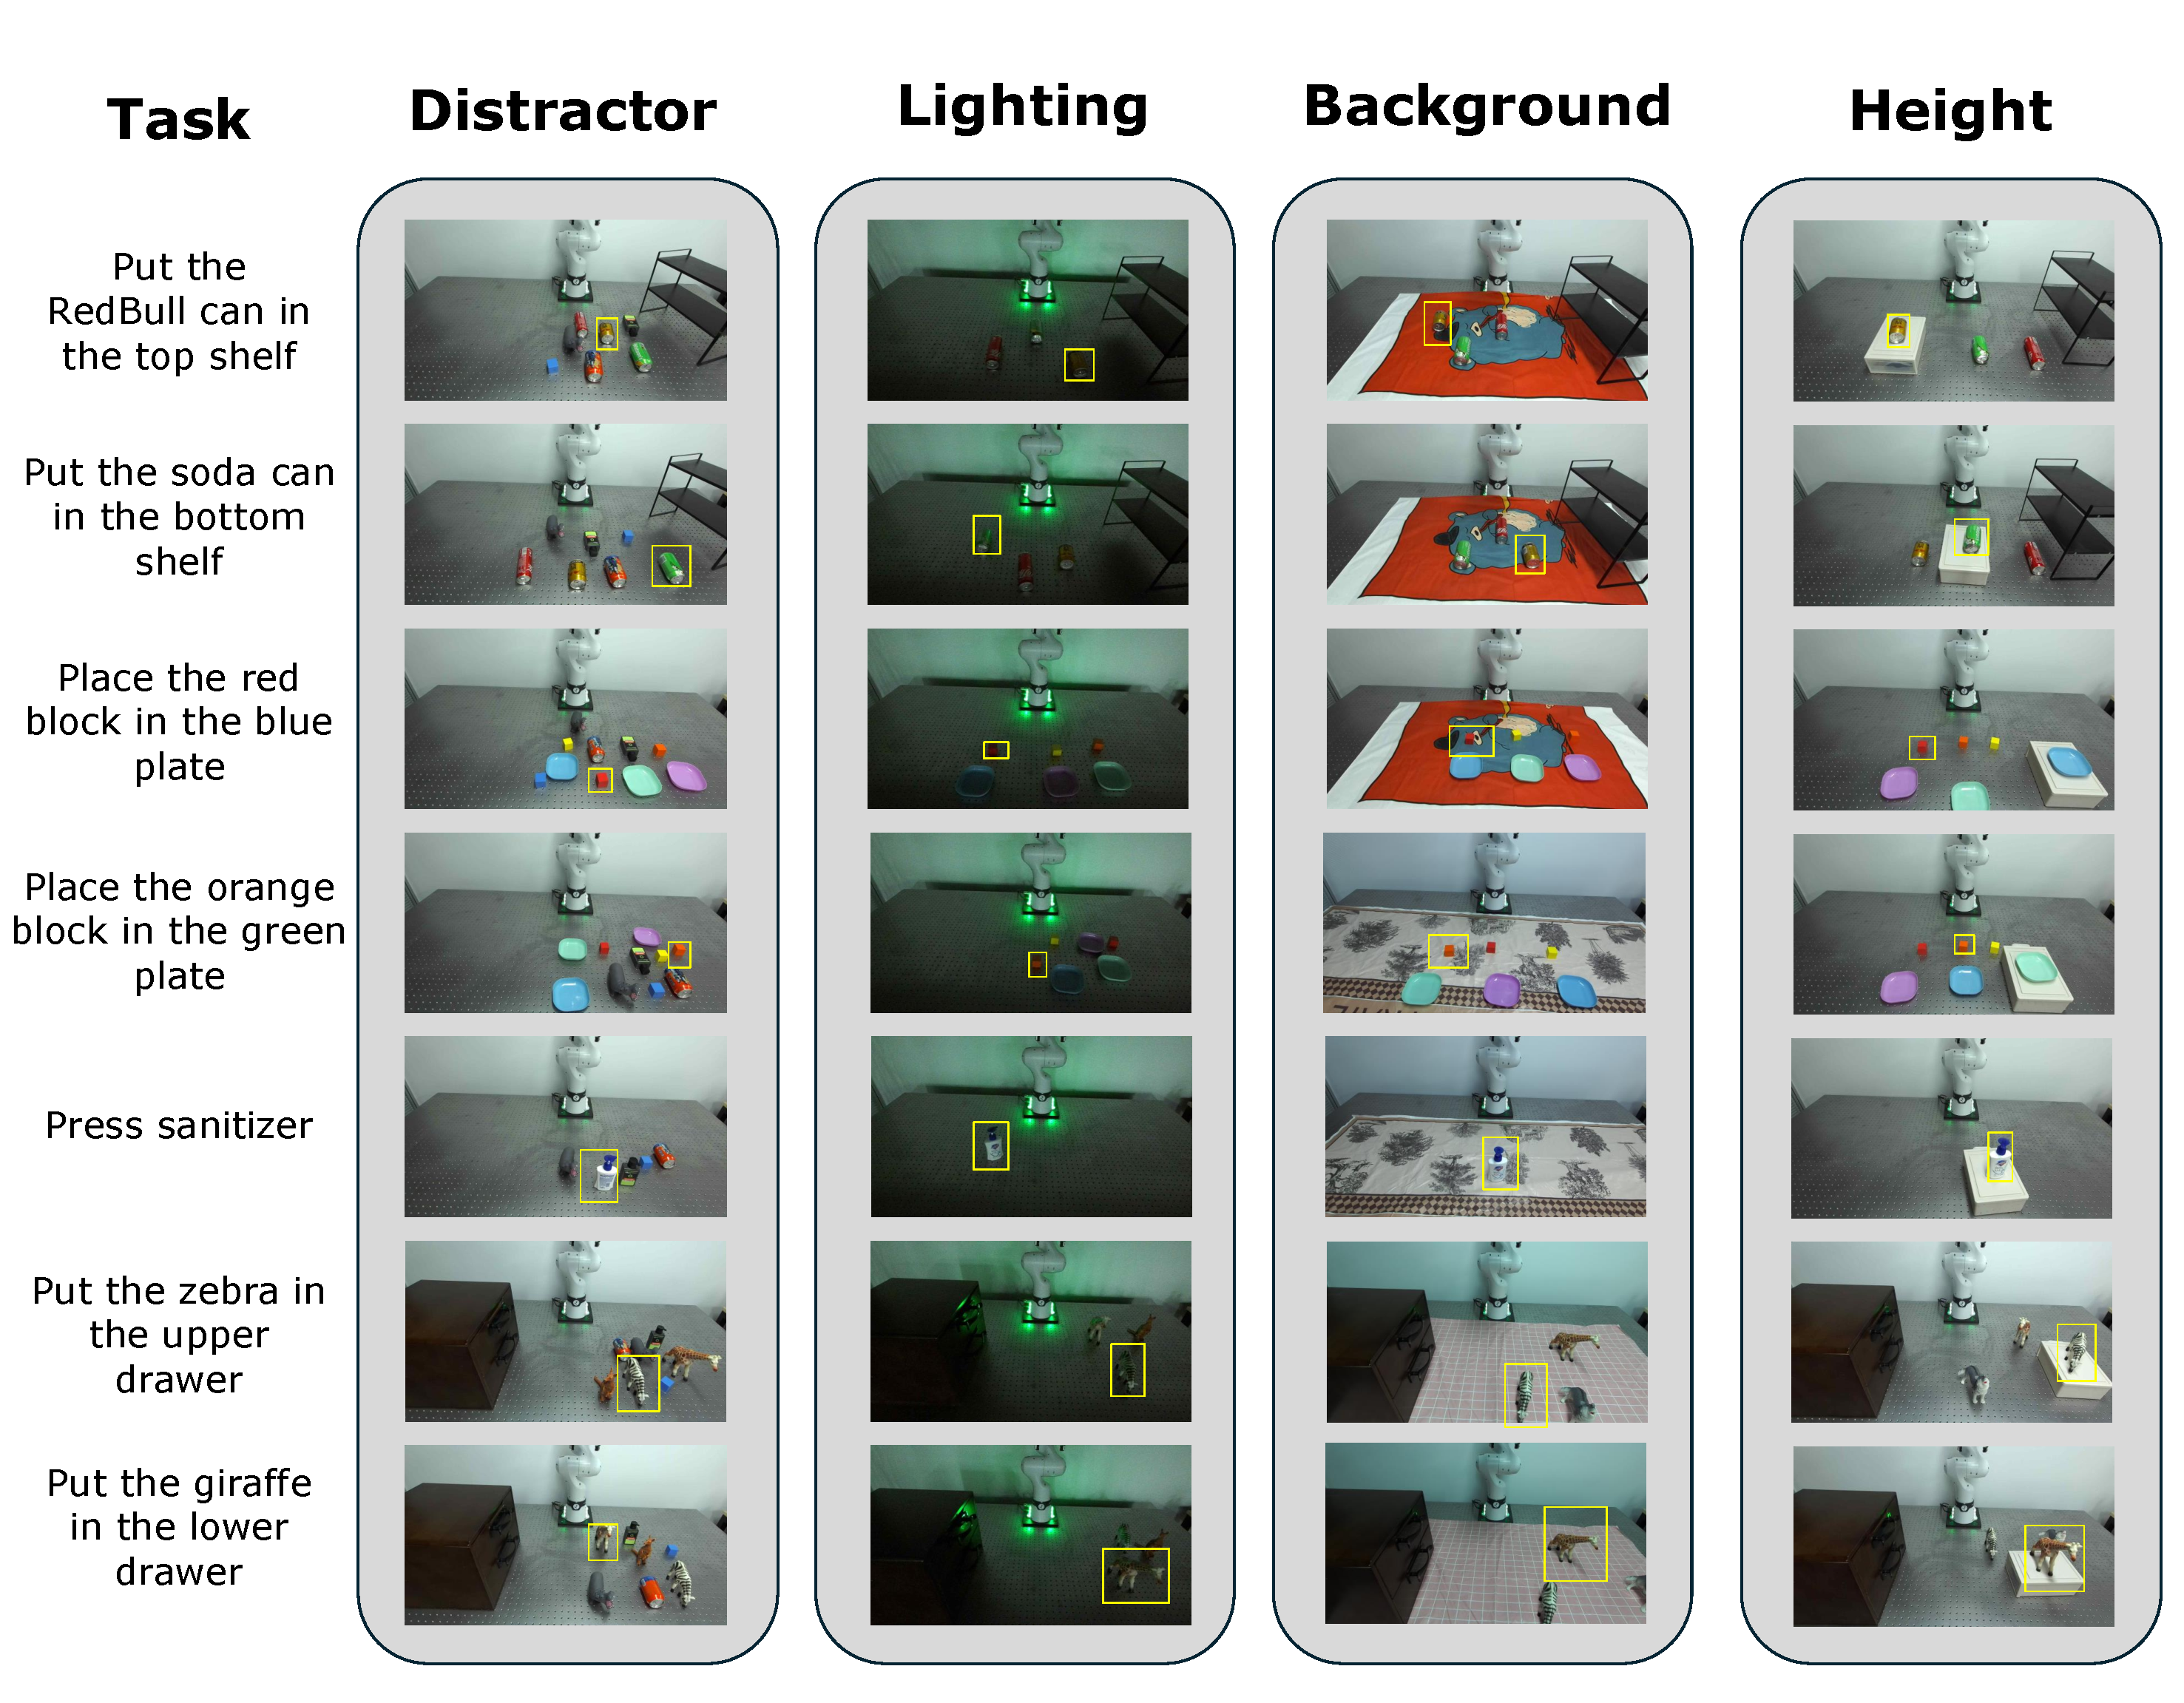
\includegraphics[width=0.72\textwidth]{figures/real_perturbation_settings.pdf}
  \caption{\textbf{The Distractor, Lighting, Background, and Height
  Settings.}
  Visualization of the four visual-disturbance settings of the
  real-robot evaluation (Appendix~\ref{app:real_franka}).}
  \label{fig:real_settings}
\end{figure*}

\begin{figure*}[t]
  \centering
  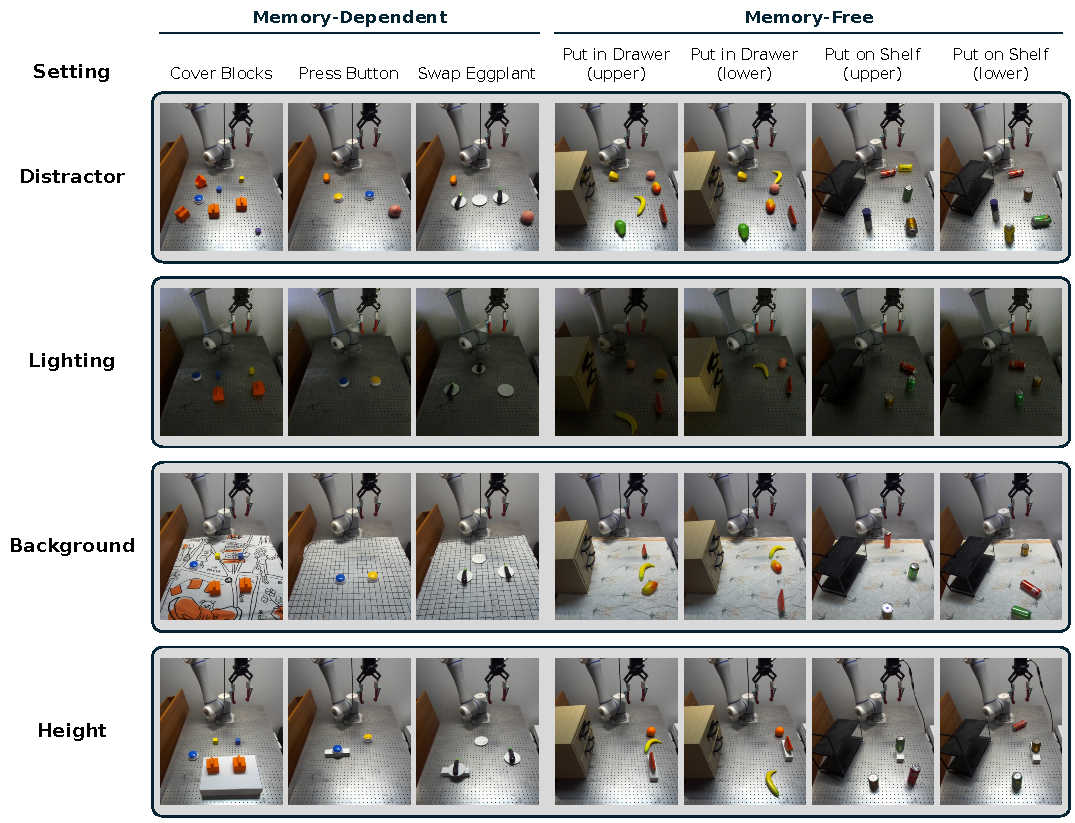
\includegraphics[width=0.72\textwidth]{figures/dobot_perturbation_settings.pdf}
  \caption{\textbf{The Distractor, Lighting, Background, and Height
  Settings on the Dobot Platform.}
  Initial scene of every instruction of the Dobot suite (columns, named
  as in Table~\ref{tab:app:real_dobot_all}) under each of the four
  visual-disturbance settings (rows;
  Appendix~\ref{app:real_dobot}).
  Frames in the \emph{Lighting} row are gamma-darkened for display
  where the camera's auto-exposure compensated for the reduced
  illumination; the policy receives the raw frames.}
  \label{fig:dobot_settings}
\end{figure*}

% Franka rollouts I (~585pt)
\begin{figure*}[t]
  \centering
  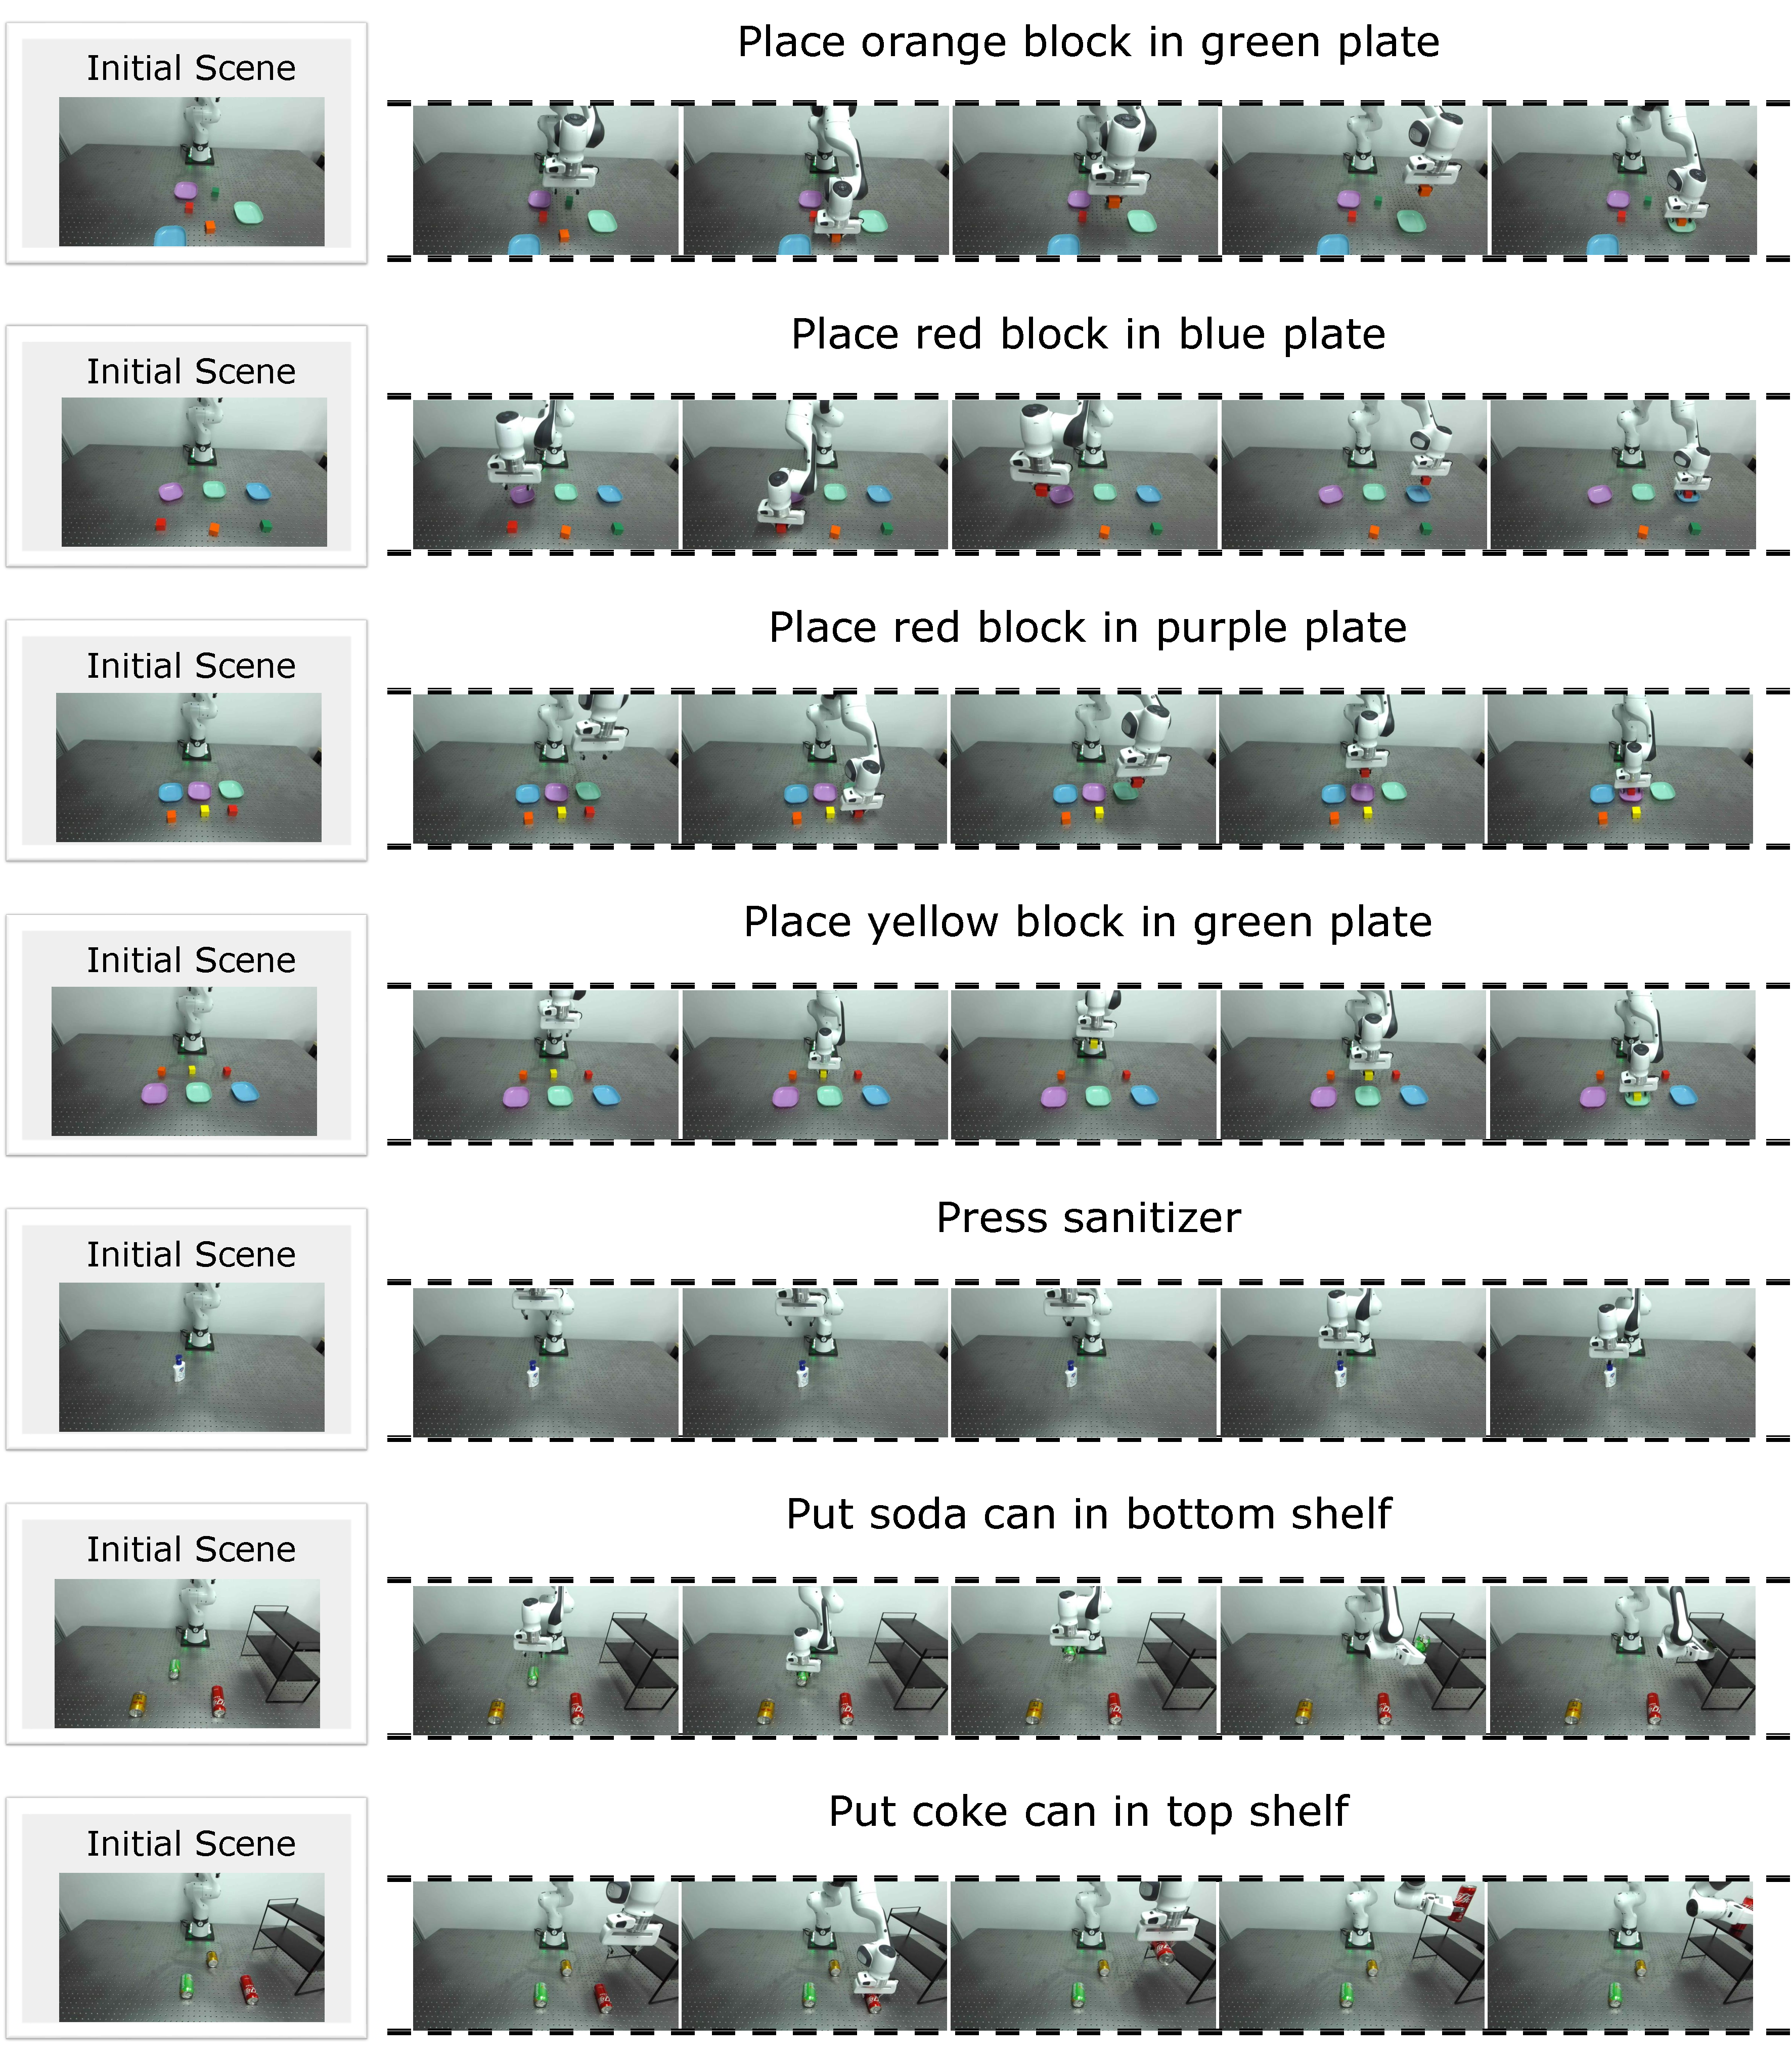
\includegraphics[width=\textwidth]{figures/real_rollouts_1.pdf}
  \caption{\textbf{Real-Robot Rollouts (I).}
  \method\ rollouts on the real-robot task suite of
  Appendix~\ref{app:real_franka}.}
  \label{fig:basic_task1}
\end{figure*}

% Franka rollouts II (~535pt)
\begin{figure*}[t]
  \centering
  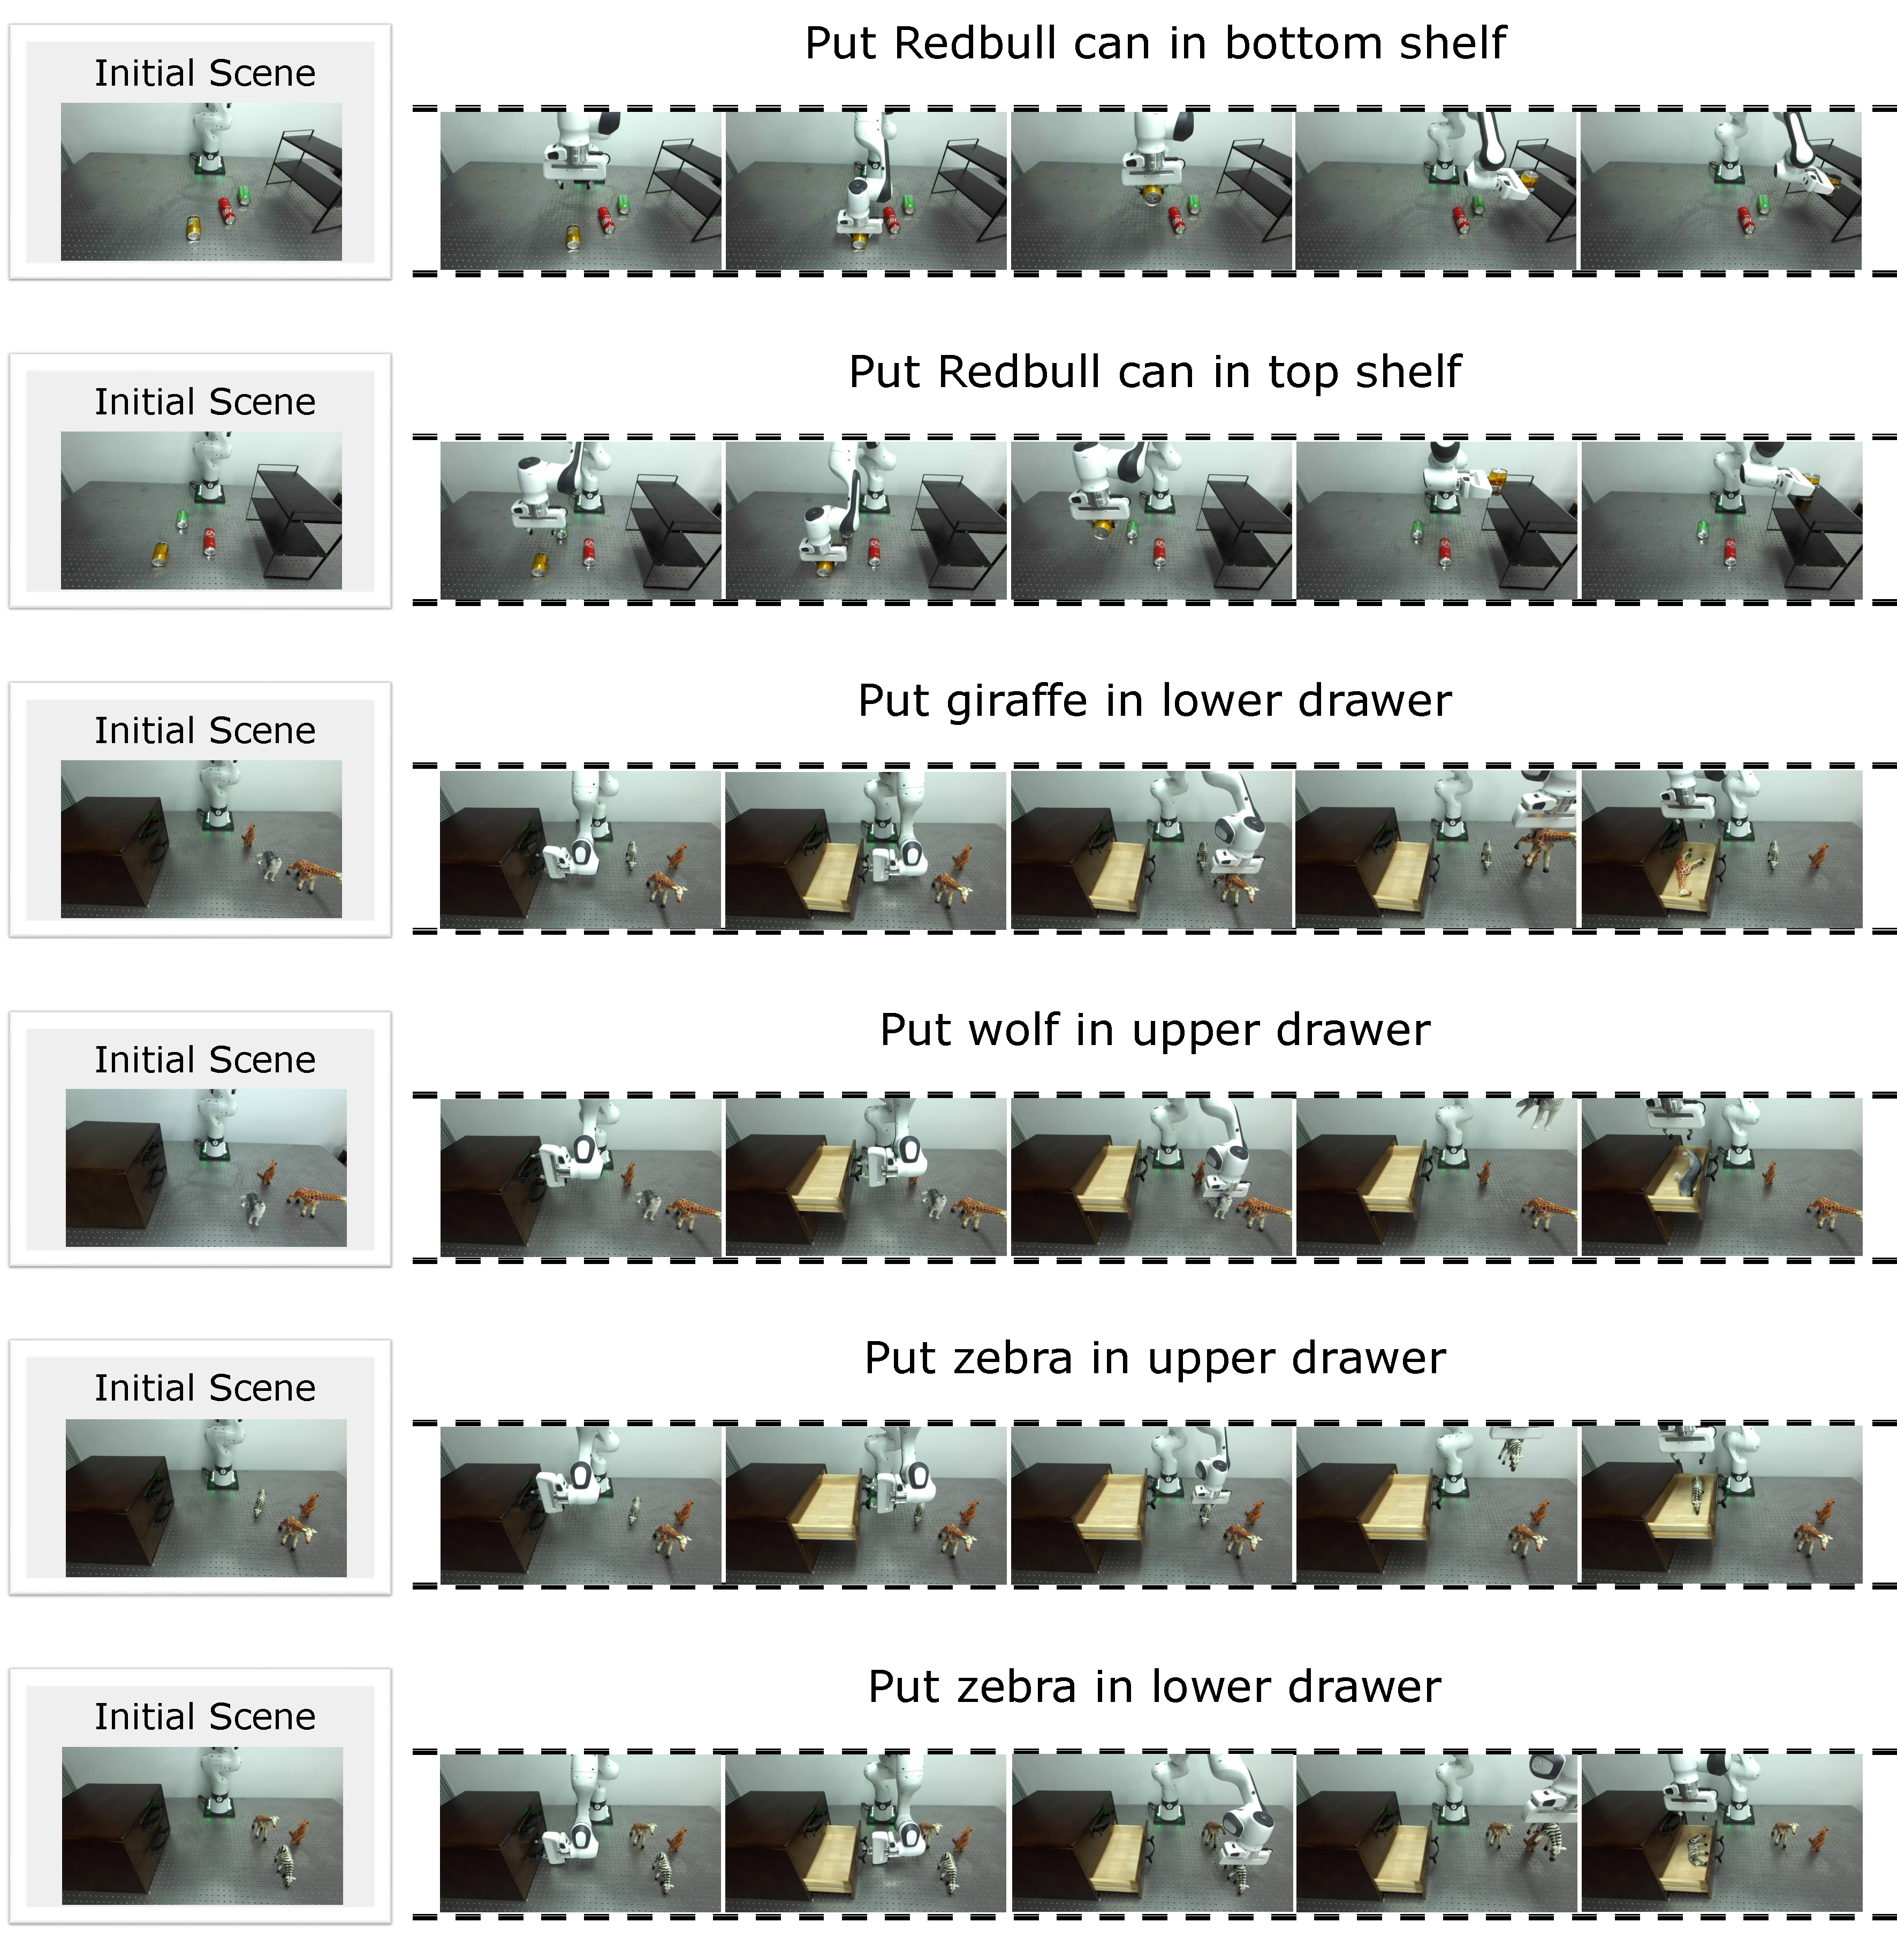
\includegraphics[width=\textwidth]{figures/real_rollouts_2.pdf}
  \caption{\textbf{Real-Robot Rollouts (II).}
  \method\ rollouts on the real-robot task suite of
  Appendix~\ref{app:real_franka}.}
  \label{fig:basic_task2}
\end{figure*}

% Combination setting I (~645pt)
\begin{figure*}[t]
  \centering
  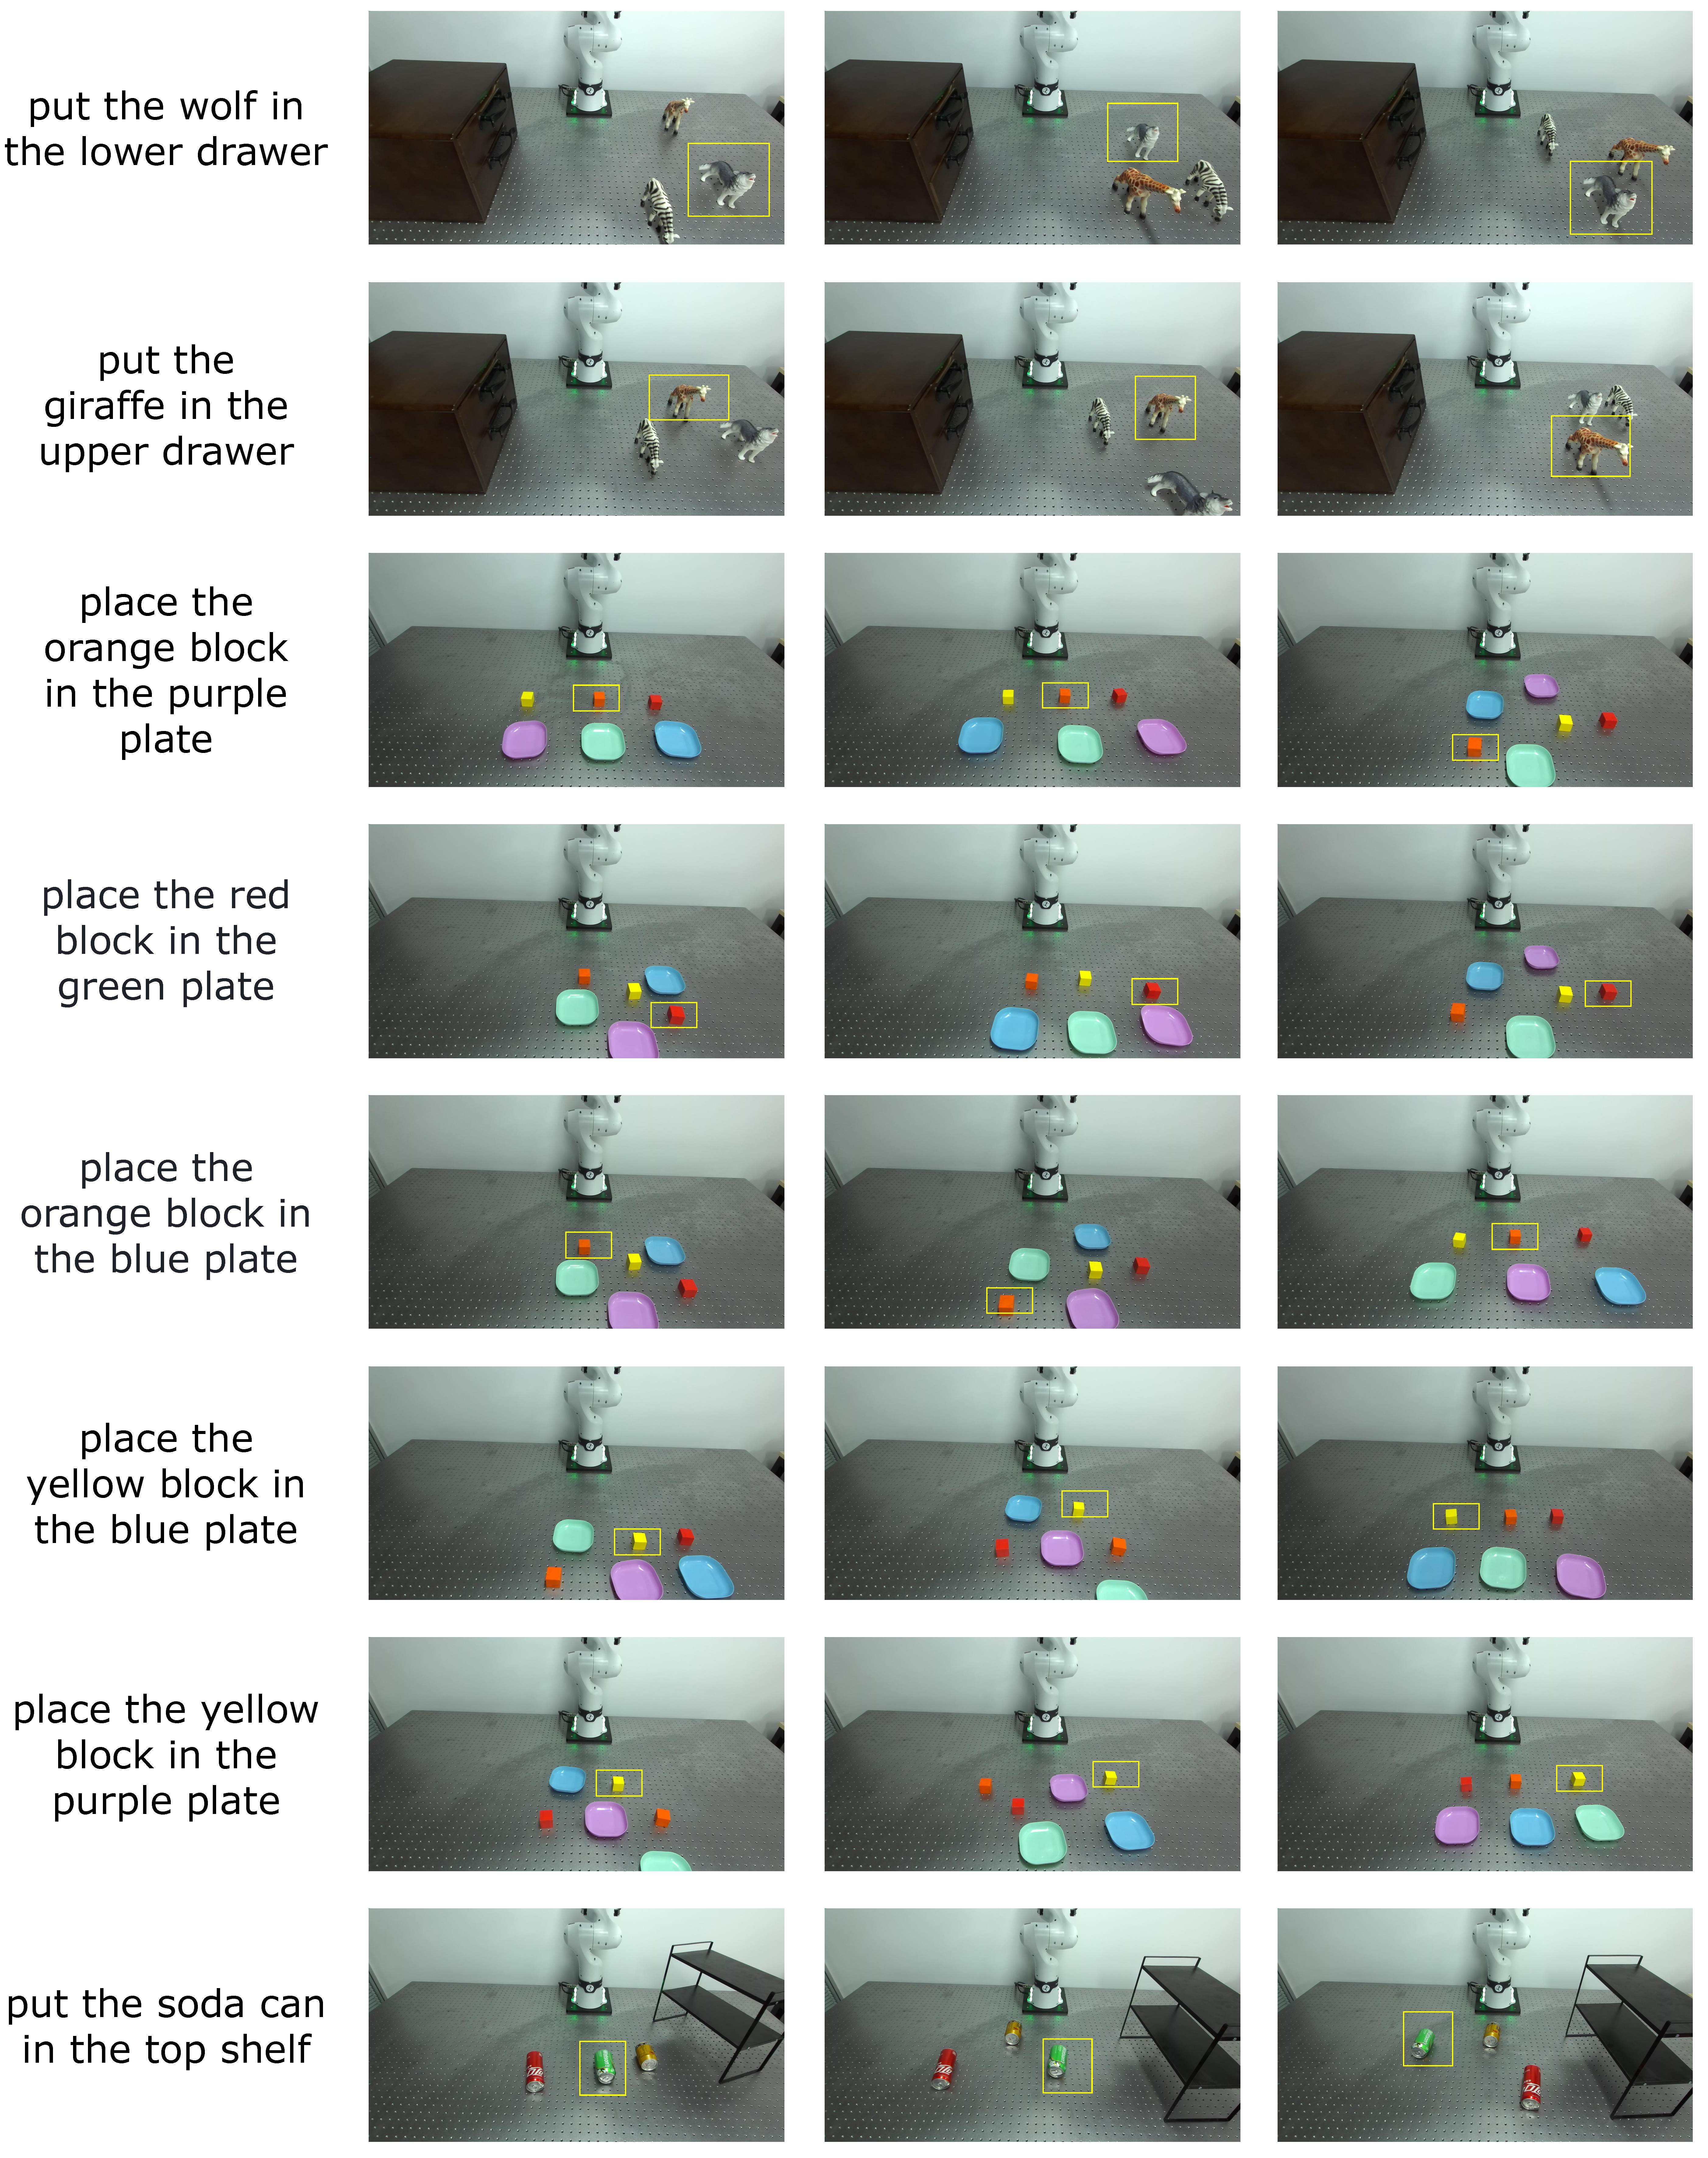
\includegraphics[width=\textwidth]{figures/combination_within.pdf}
  \caption{\textbf{The Combination Setting (I).}
  During training, the manipulated objects and skills are seen, but
  their combinations are unseen.}
  \label{fig:combination_within}
\end{figure*}

% p7: Combination setting II (~420pt) + 3-vs-10-demonstration table (~130pt)
\begin{figure*}[t]
  \centering
  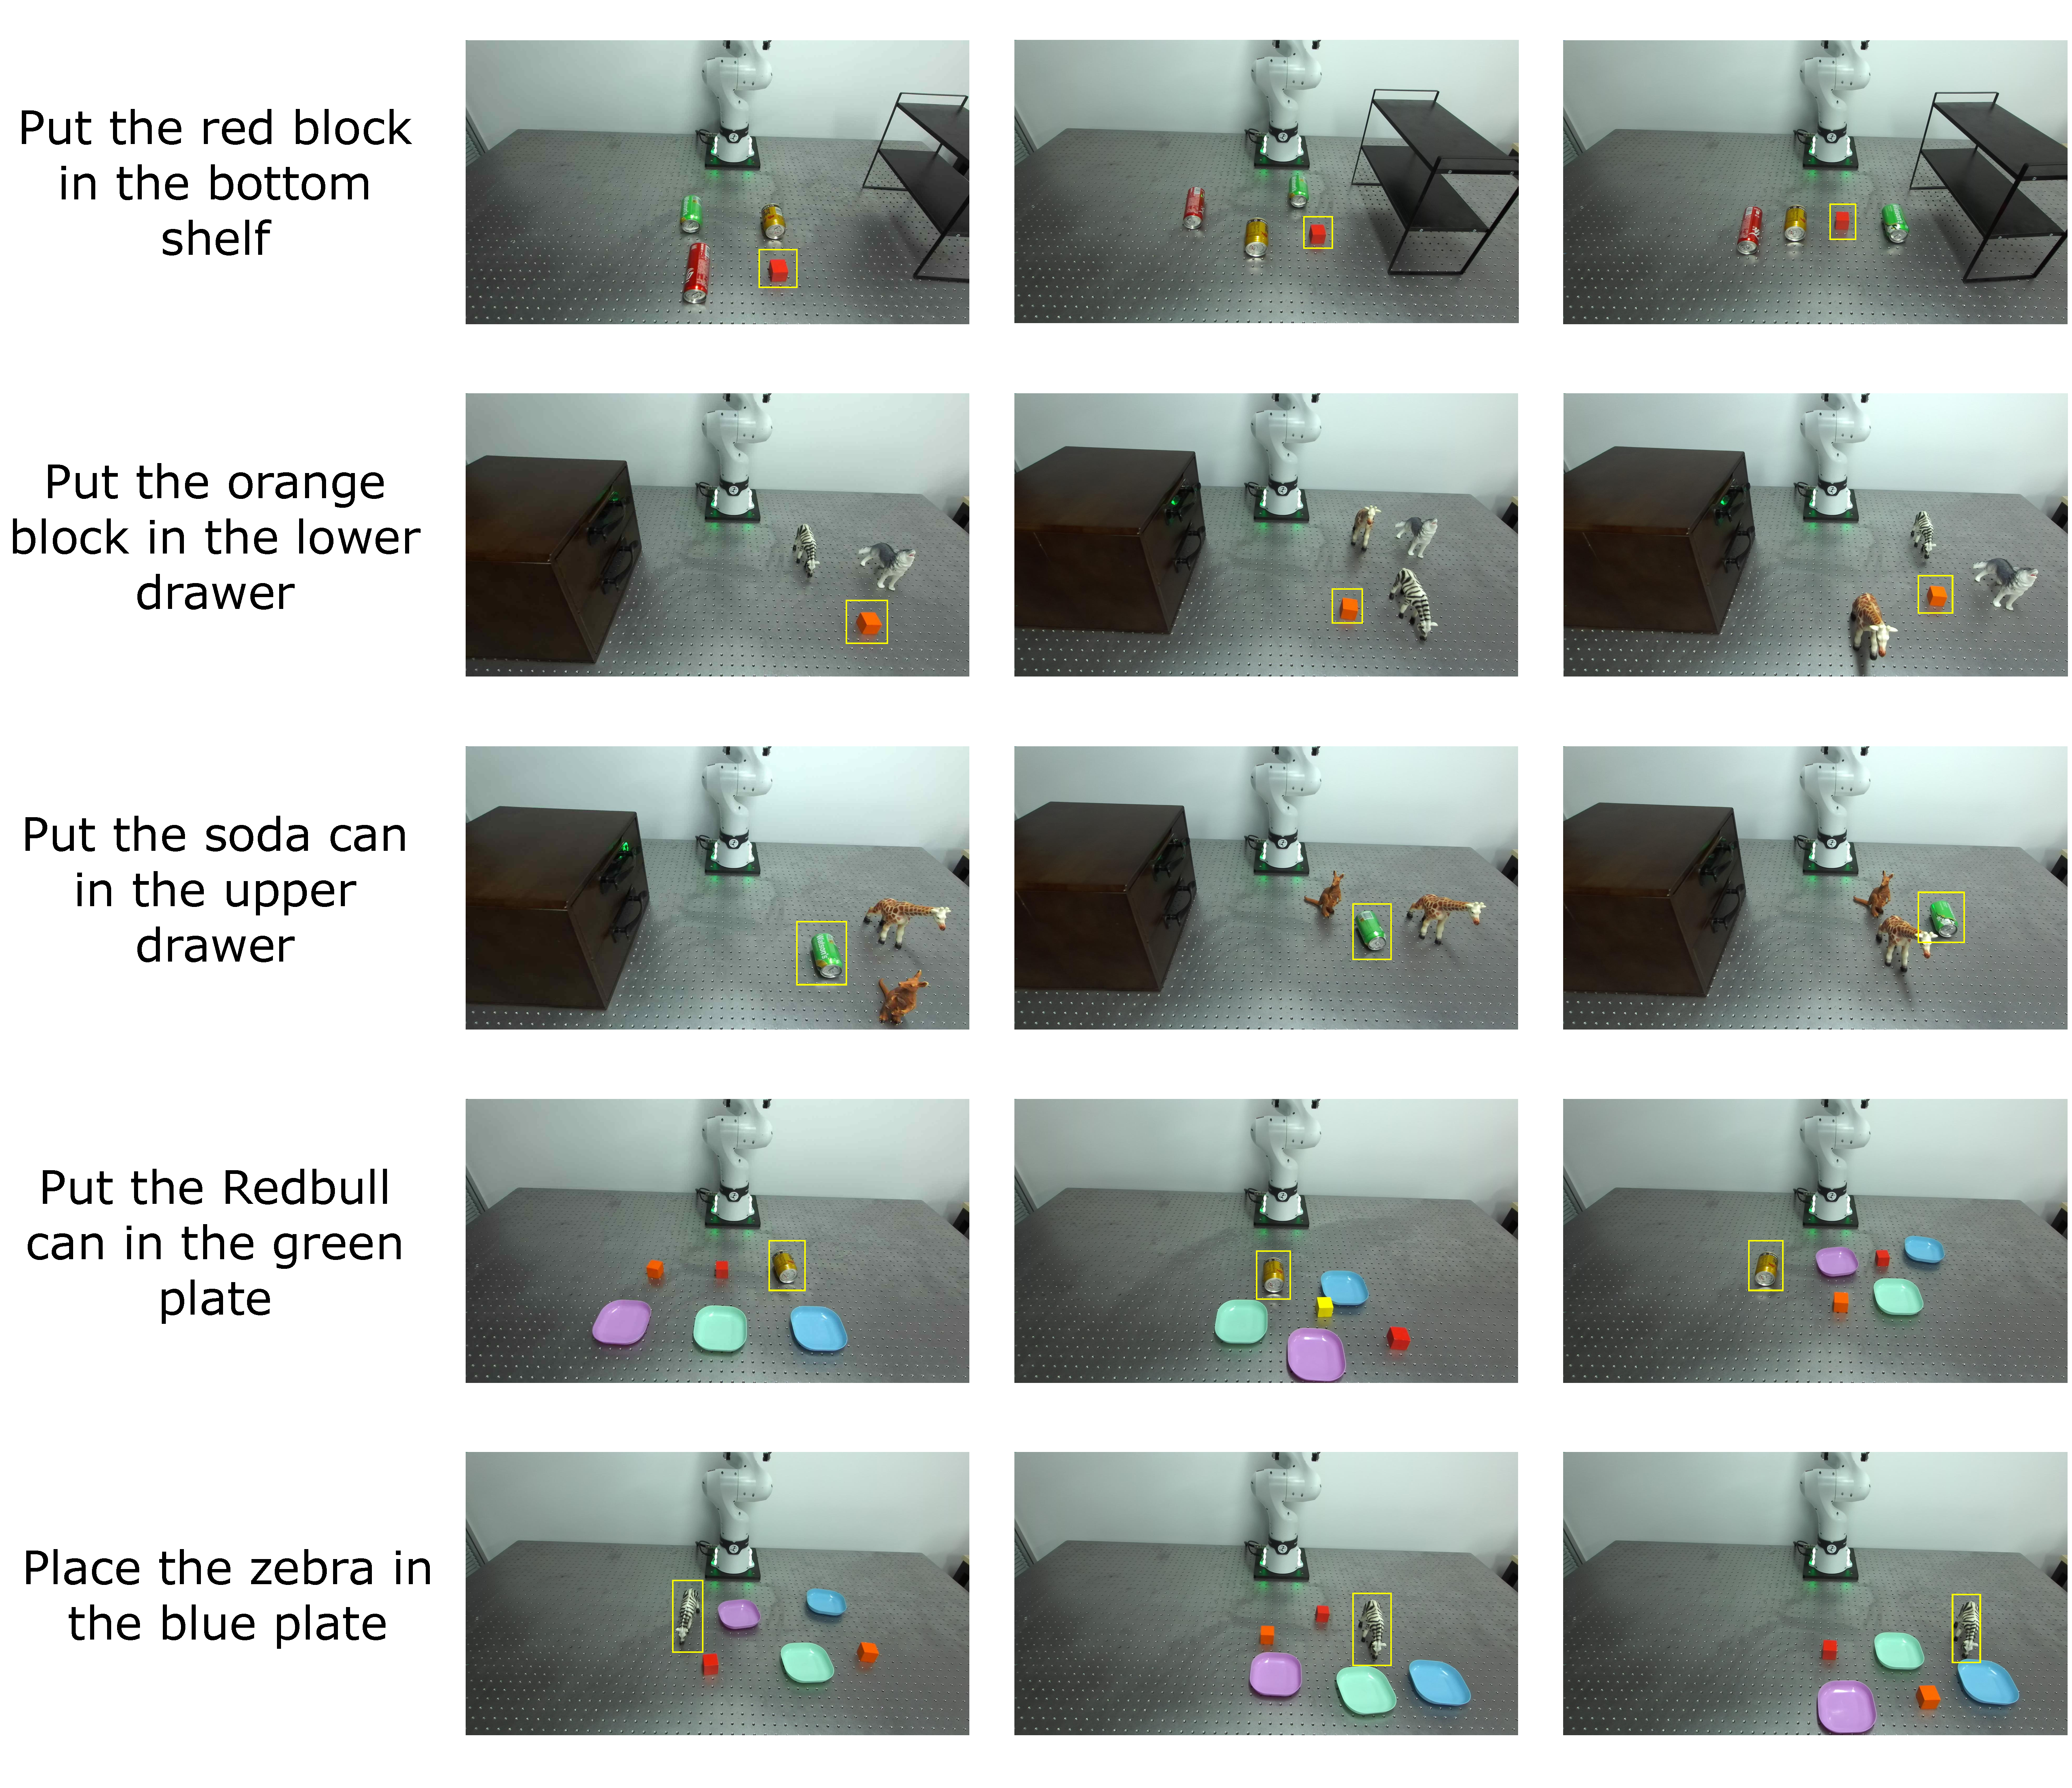
\includegraphics[width=\textwidth]{figures/combination_across.pdf}
  \caption{\textbf{The Combination Setting (II).}
  During training, the manipulated objects and skills are seen, but
  their combinations are unseen.}
  \label{fig:combination_across}
\end{figure*}

% Category setting (~535pt at 0.85\textwidth)
\begin{figure*}[t]
  \centering
  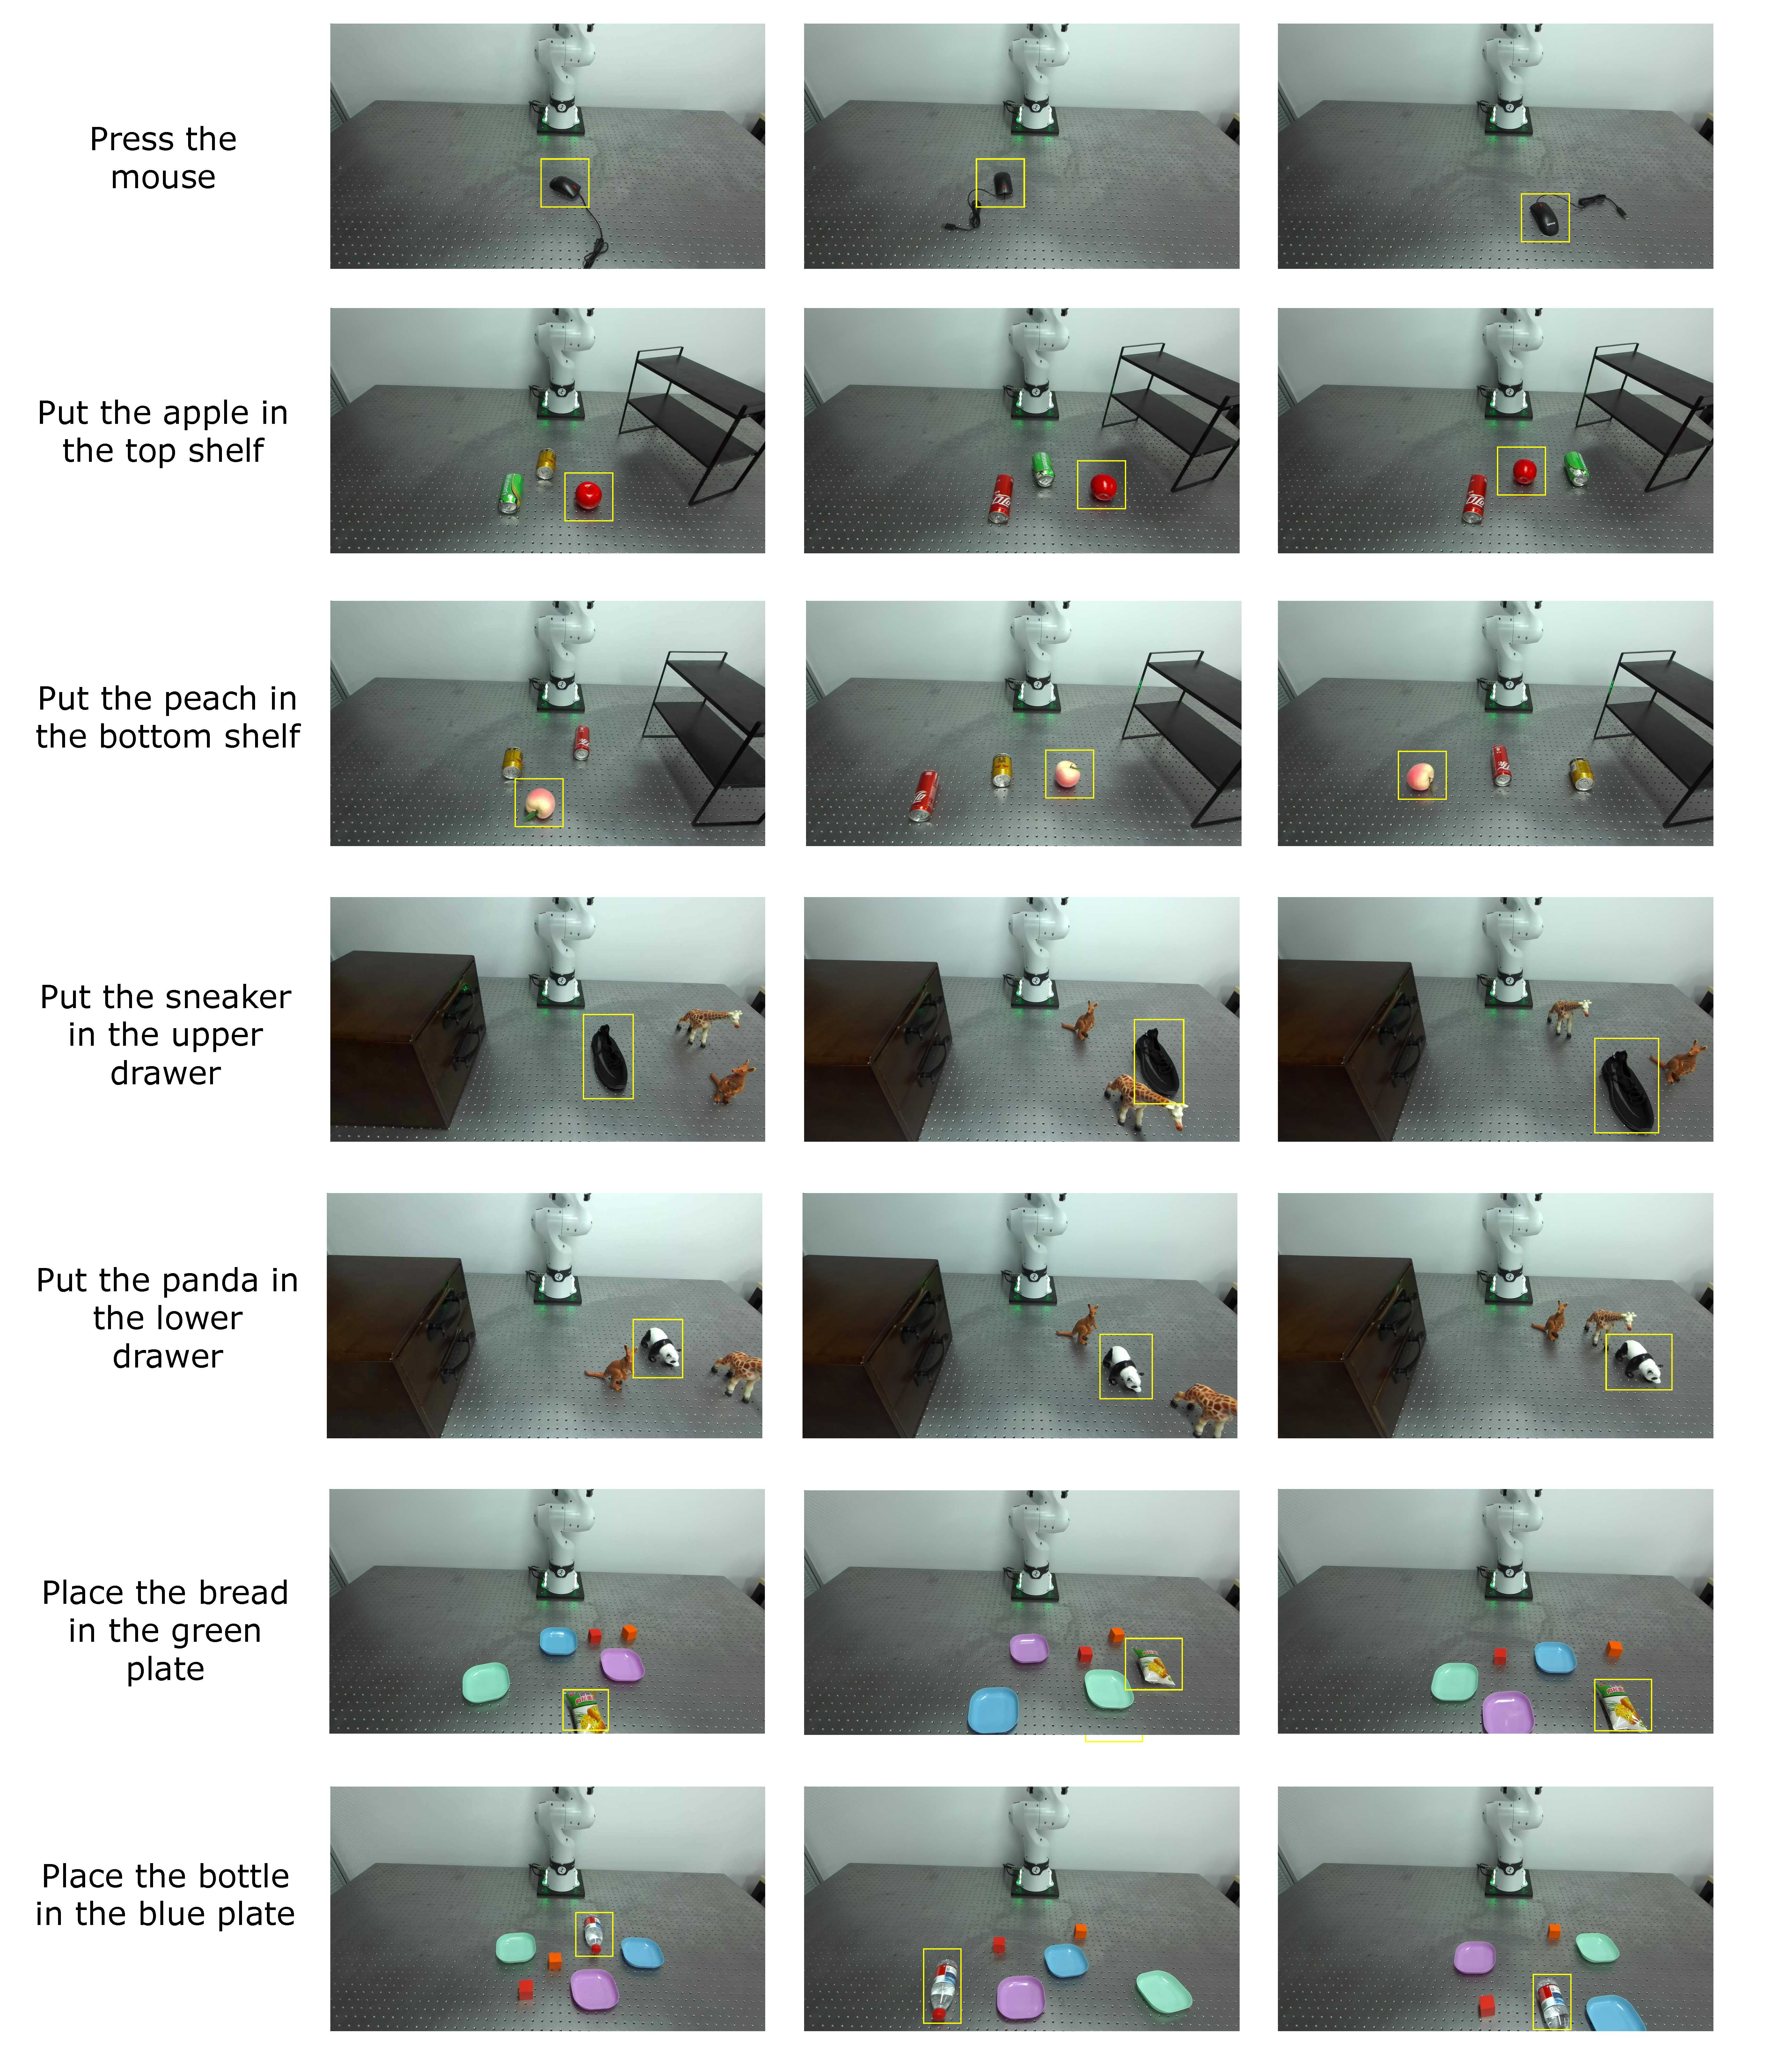
\includegraphics[width=0.85\textwidth]{figures/category_setting.pdf}
  \caption{\textbf{The Category Setting.}
  In total, we evaluate on 7 objects from categories that are unseen
  during training.}
  \label{fig:category}
\end{figure*}

% Dobot rollouts I + II paired on one page: both shrunk to 0.62\tw so their
% combined height (~660pt incl. captions) fits a single float page.
\begin{figure*}[t]
  \centering
  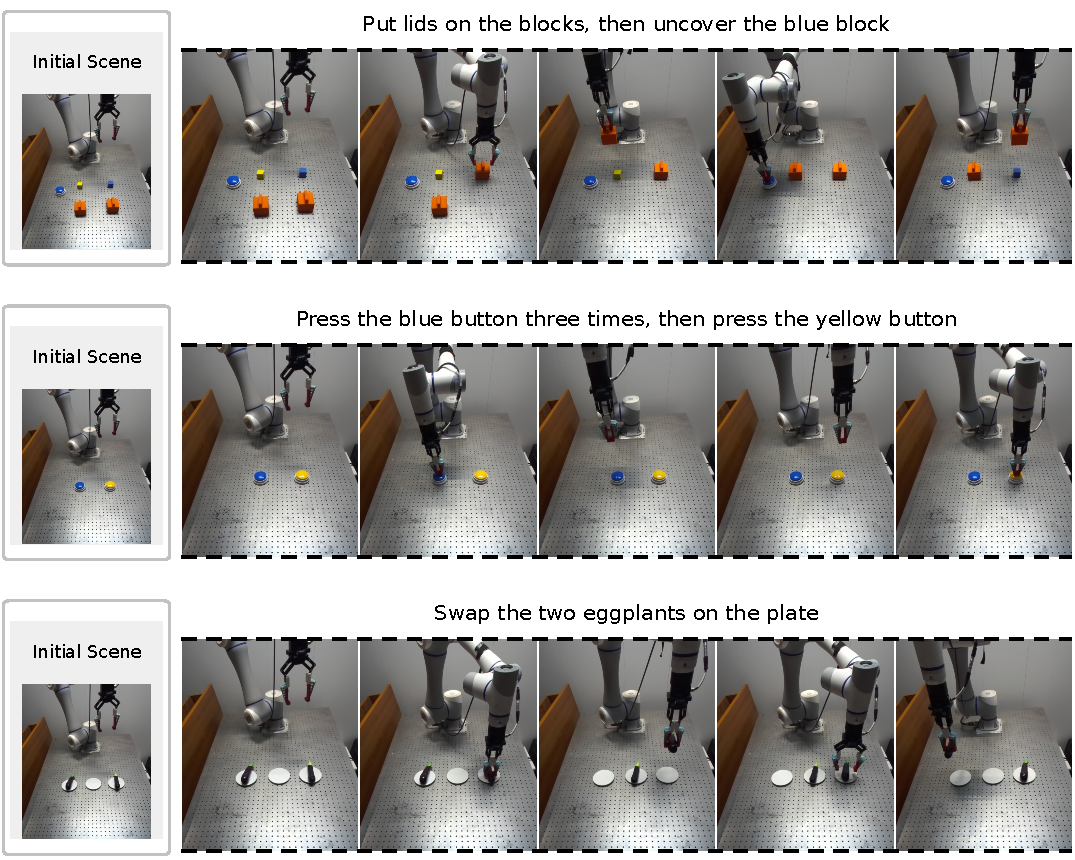
\includegraphics[width=0.62\textwidth]{figures/dobot_rollouts_1.pdf}
  \caption{\textbf{Dobot Rollouts (I): Memory-Dependent Tasks.}
  \memmethod\ rollouts on the three memory-dependent instructions of
  the Dobot suite (Appendix~\ref{app:real_dobot}) in the Basic
  setting; each strip shows five keyframes of one successful episode.}
  \label{fig:dobot_rollouts1}
\end{figure*}

% p10: Dobot rollouts II (~560pt)
\begin{figure*}[t]
  \centering
  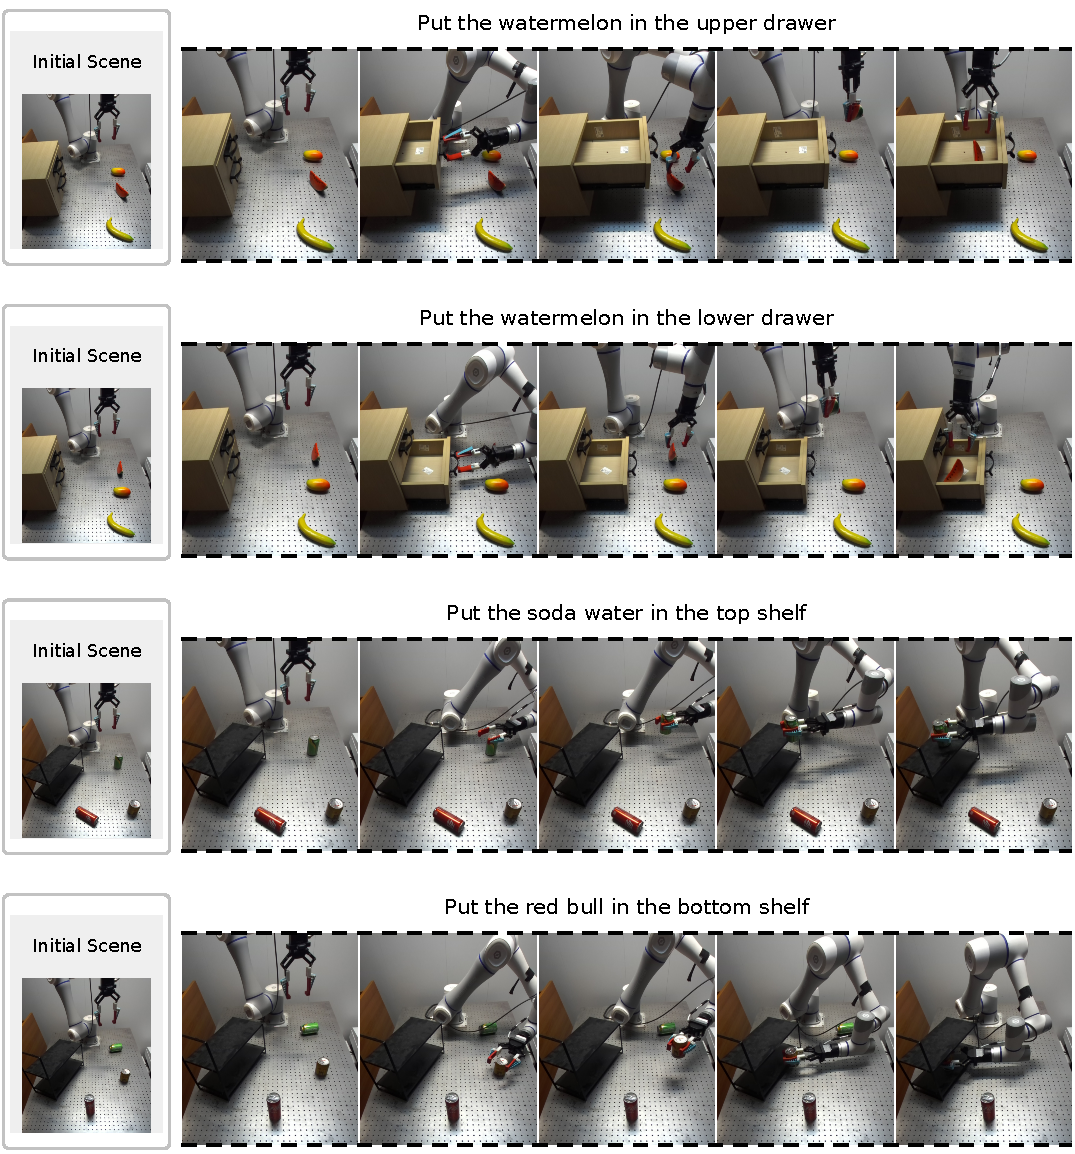
\includegraphics[width=0.62\textwidth]{figures/dobot_rollouts_2.pdf}
  \caption{\textbf{Dobot Rollouts (II): Memory-Free Tasks.}
  \memmethod\ rollouts on the four memory-free instructions of the
  Dobot suite in the Basic setting, laid out as in
  Fig.~\ref{fig:dobot_rollouts1}.}
  \label{fig:dobot_rollouts2}
\end{figure*}

% Pre-training heatmap figures: placed after the real-robot figures and
% before the simulation task grids (both are ~one full page, solo).
\begin{figure*}[t]
  \centering
  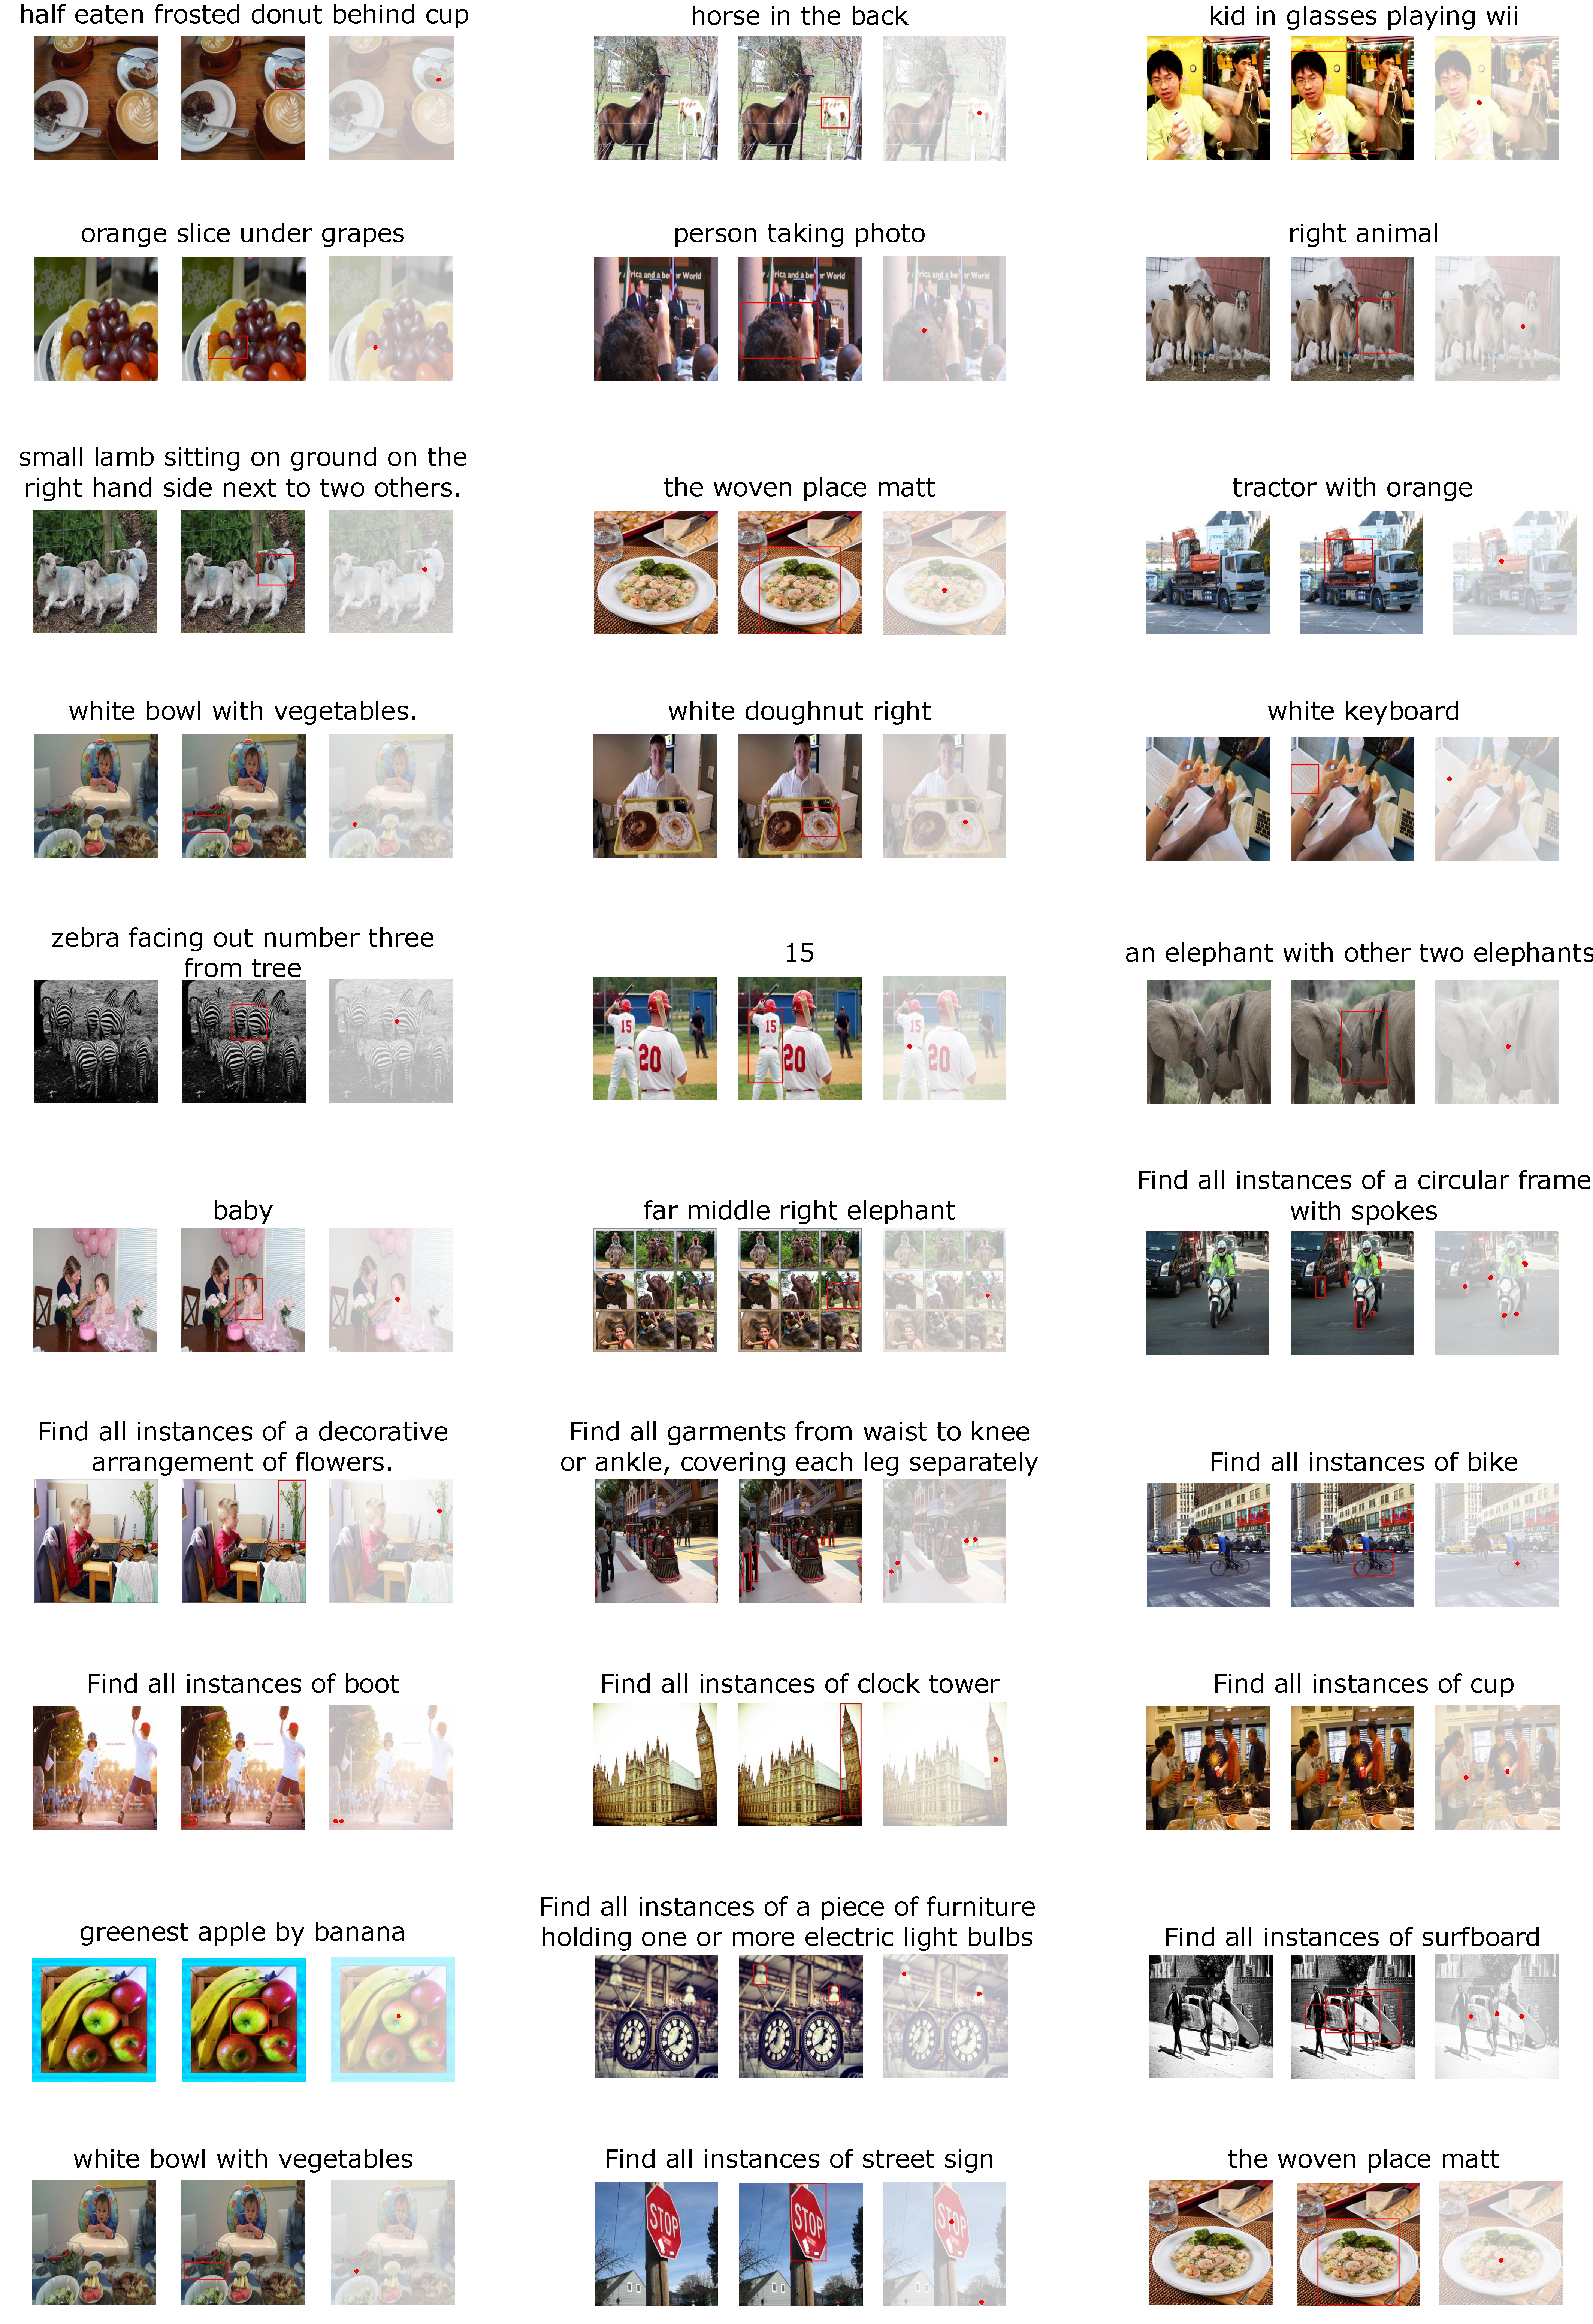
\includegraphics[width=0.85\textwidth]{figures/pretrain_dataset.pdf}
  \caption{\textbf{Ground-Truth Heatmap Construction on Detection
  Data.}
  For each sample: the original image (\emph{left}), the bounding
  boxes of the objects of interest (\emph{middle}), and the
  ground-truth heatmap rendered from the box centers (\emph{right}).}
  \label{fig:pretrain_dataset}
\end{figure*}

\begin{figure*}[t]
  \centering
  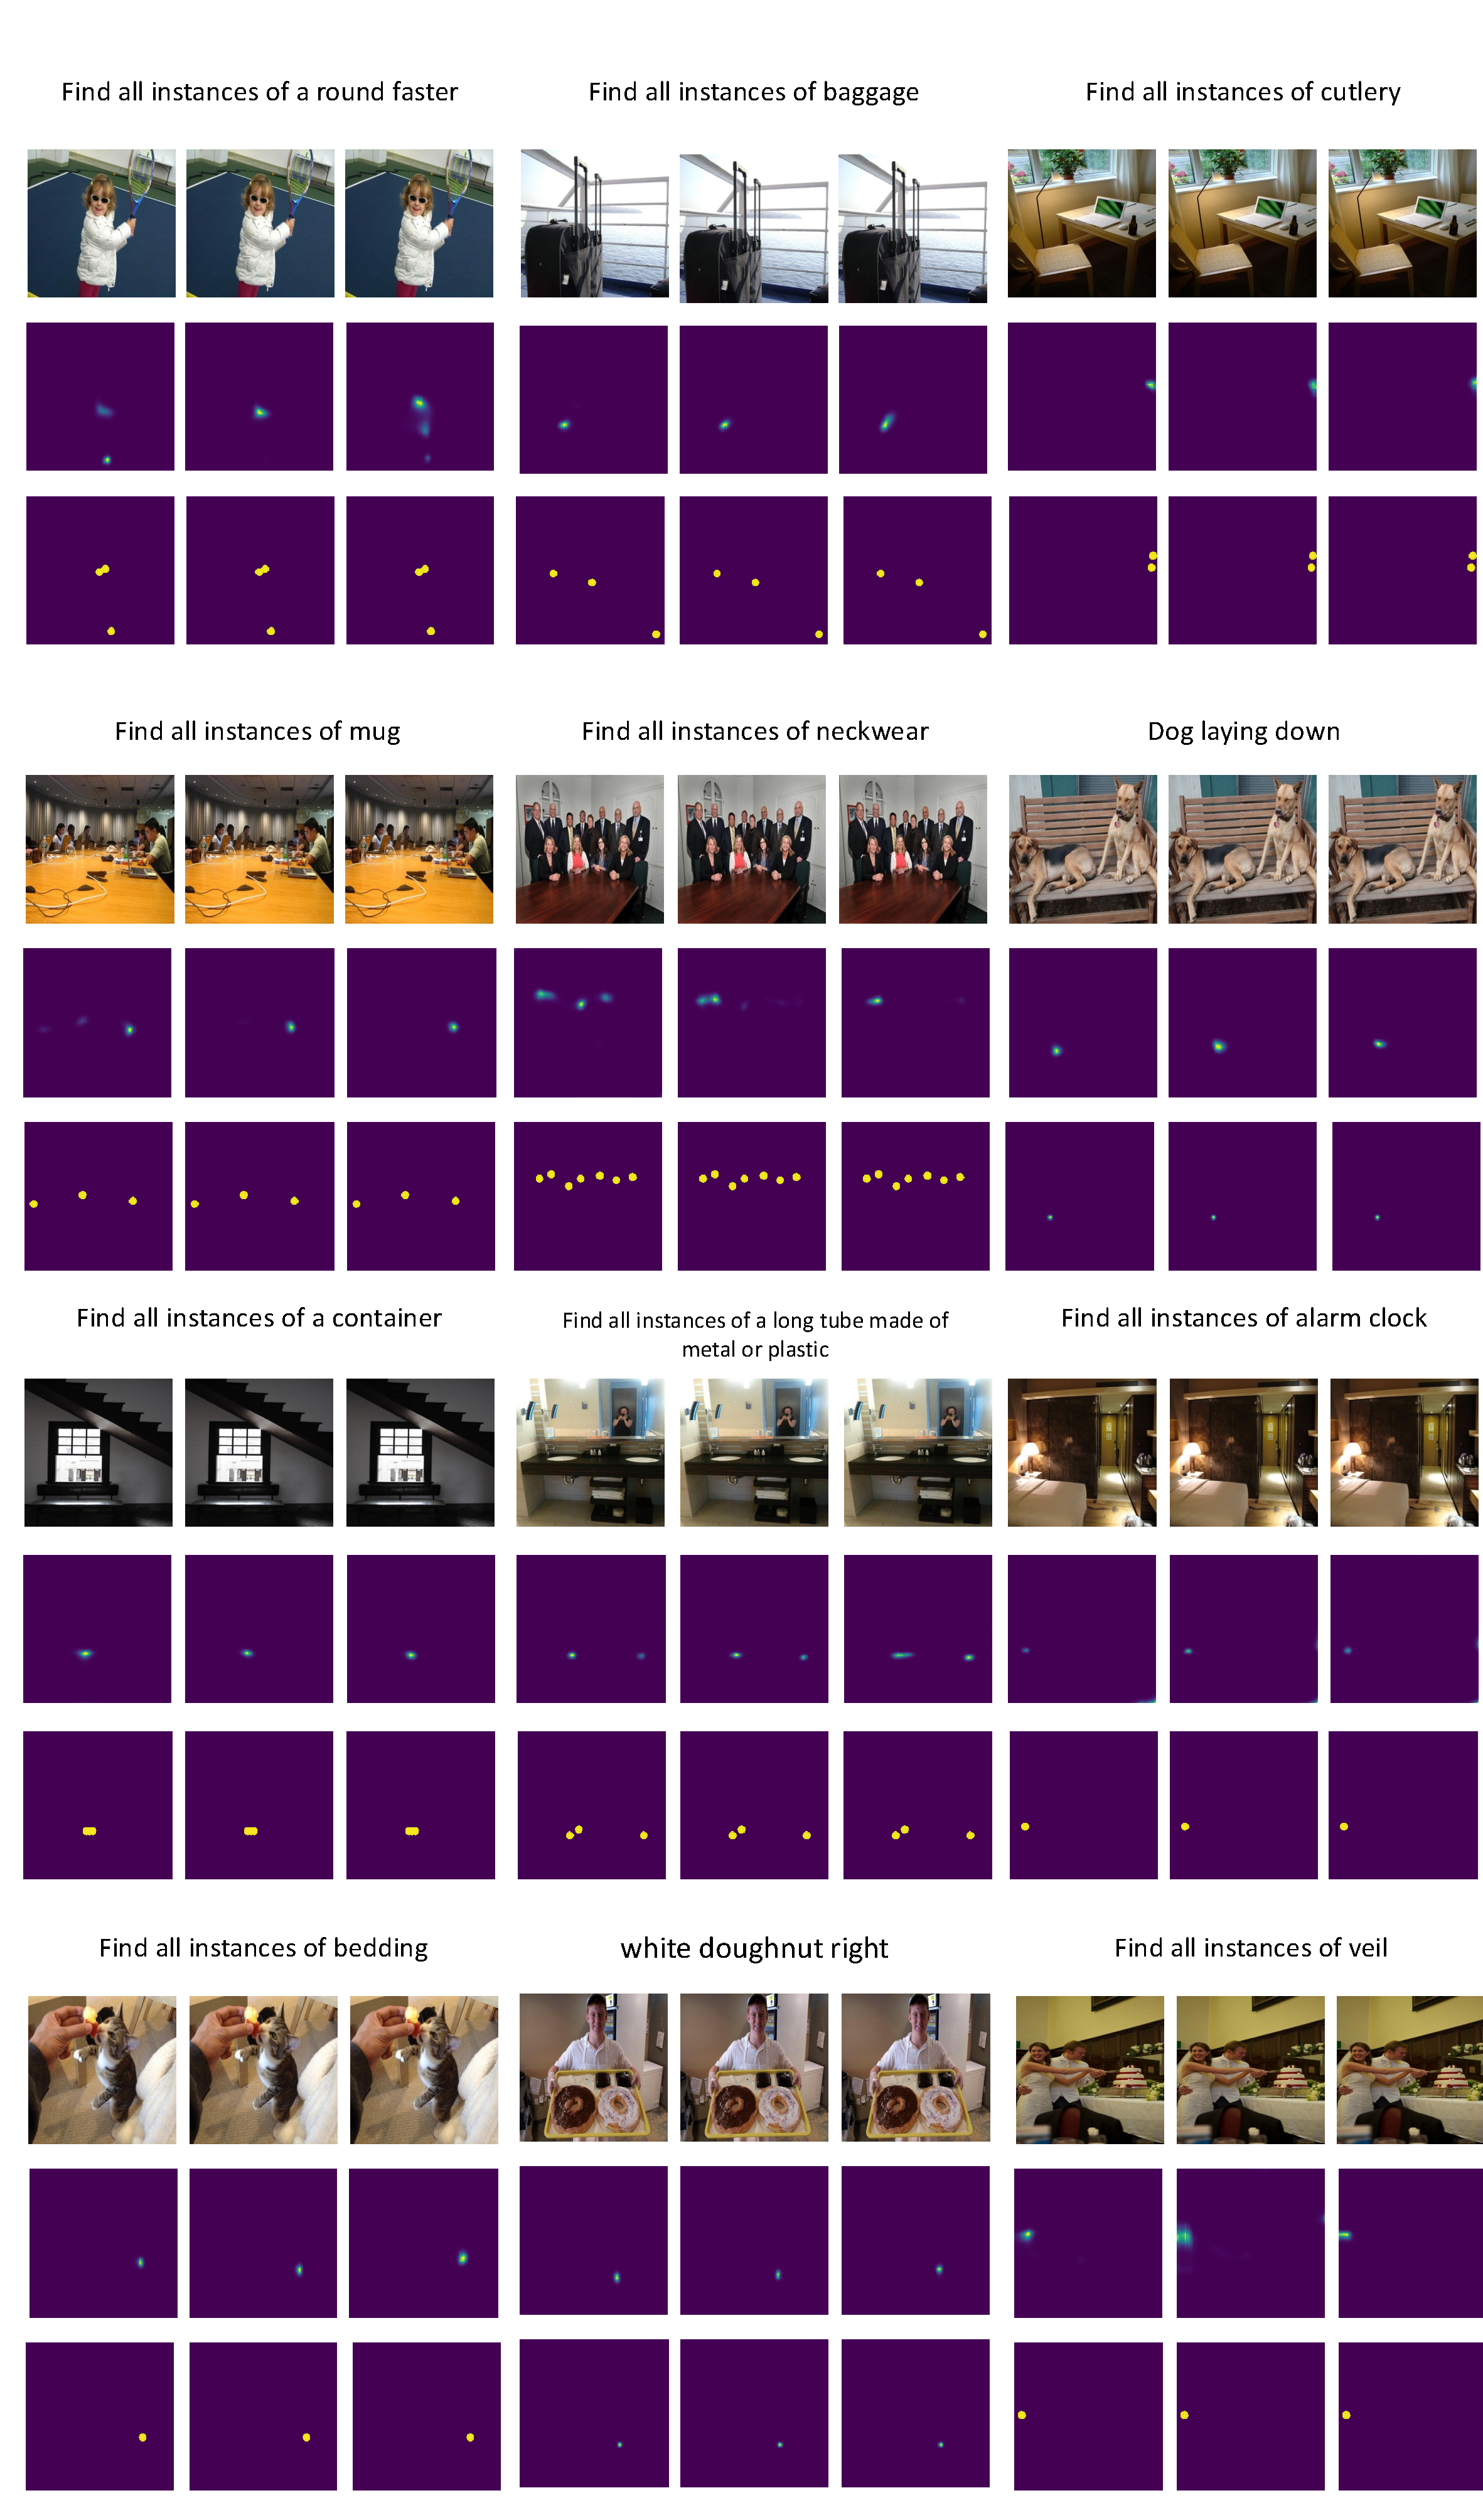
\includegraphics[width=0.72\textwidth]{figures/pred_heatmap.pdf}
  \caption{\textbf{Predictions on Pre-Training Data after
  Fine-Tuning.}
  Each input image is repeated three times to mimic the multi-view
  input format of fine-tuning.
  Rows per sample: input image, predicted heatmaps, ground truth.
  Samples are not cherry-picked.}
  \label{fig:real_heatmaps}
\end{figure*}

% --- Simulation task grids ---
% RLBench task grid (~400pt) + RMBench task grid (~195pt)
\begin{figure*}[t]
  \centering
  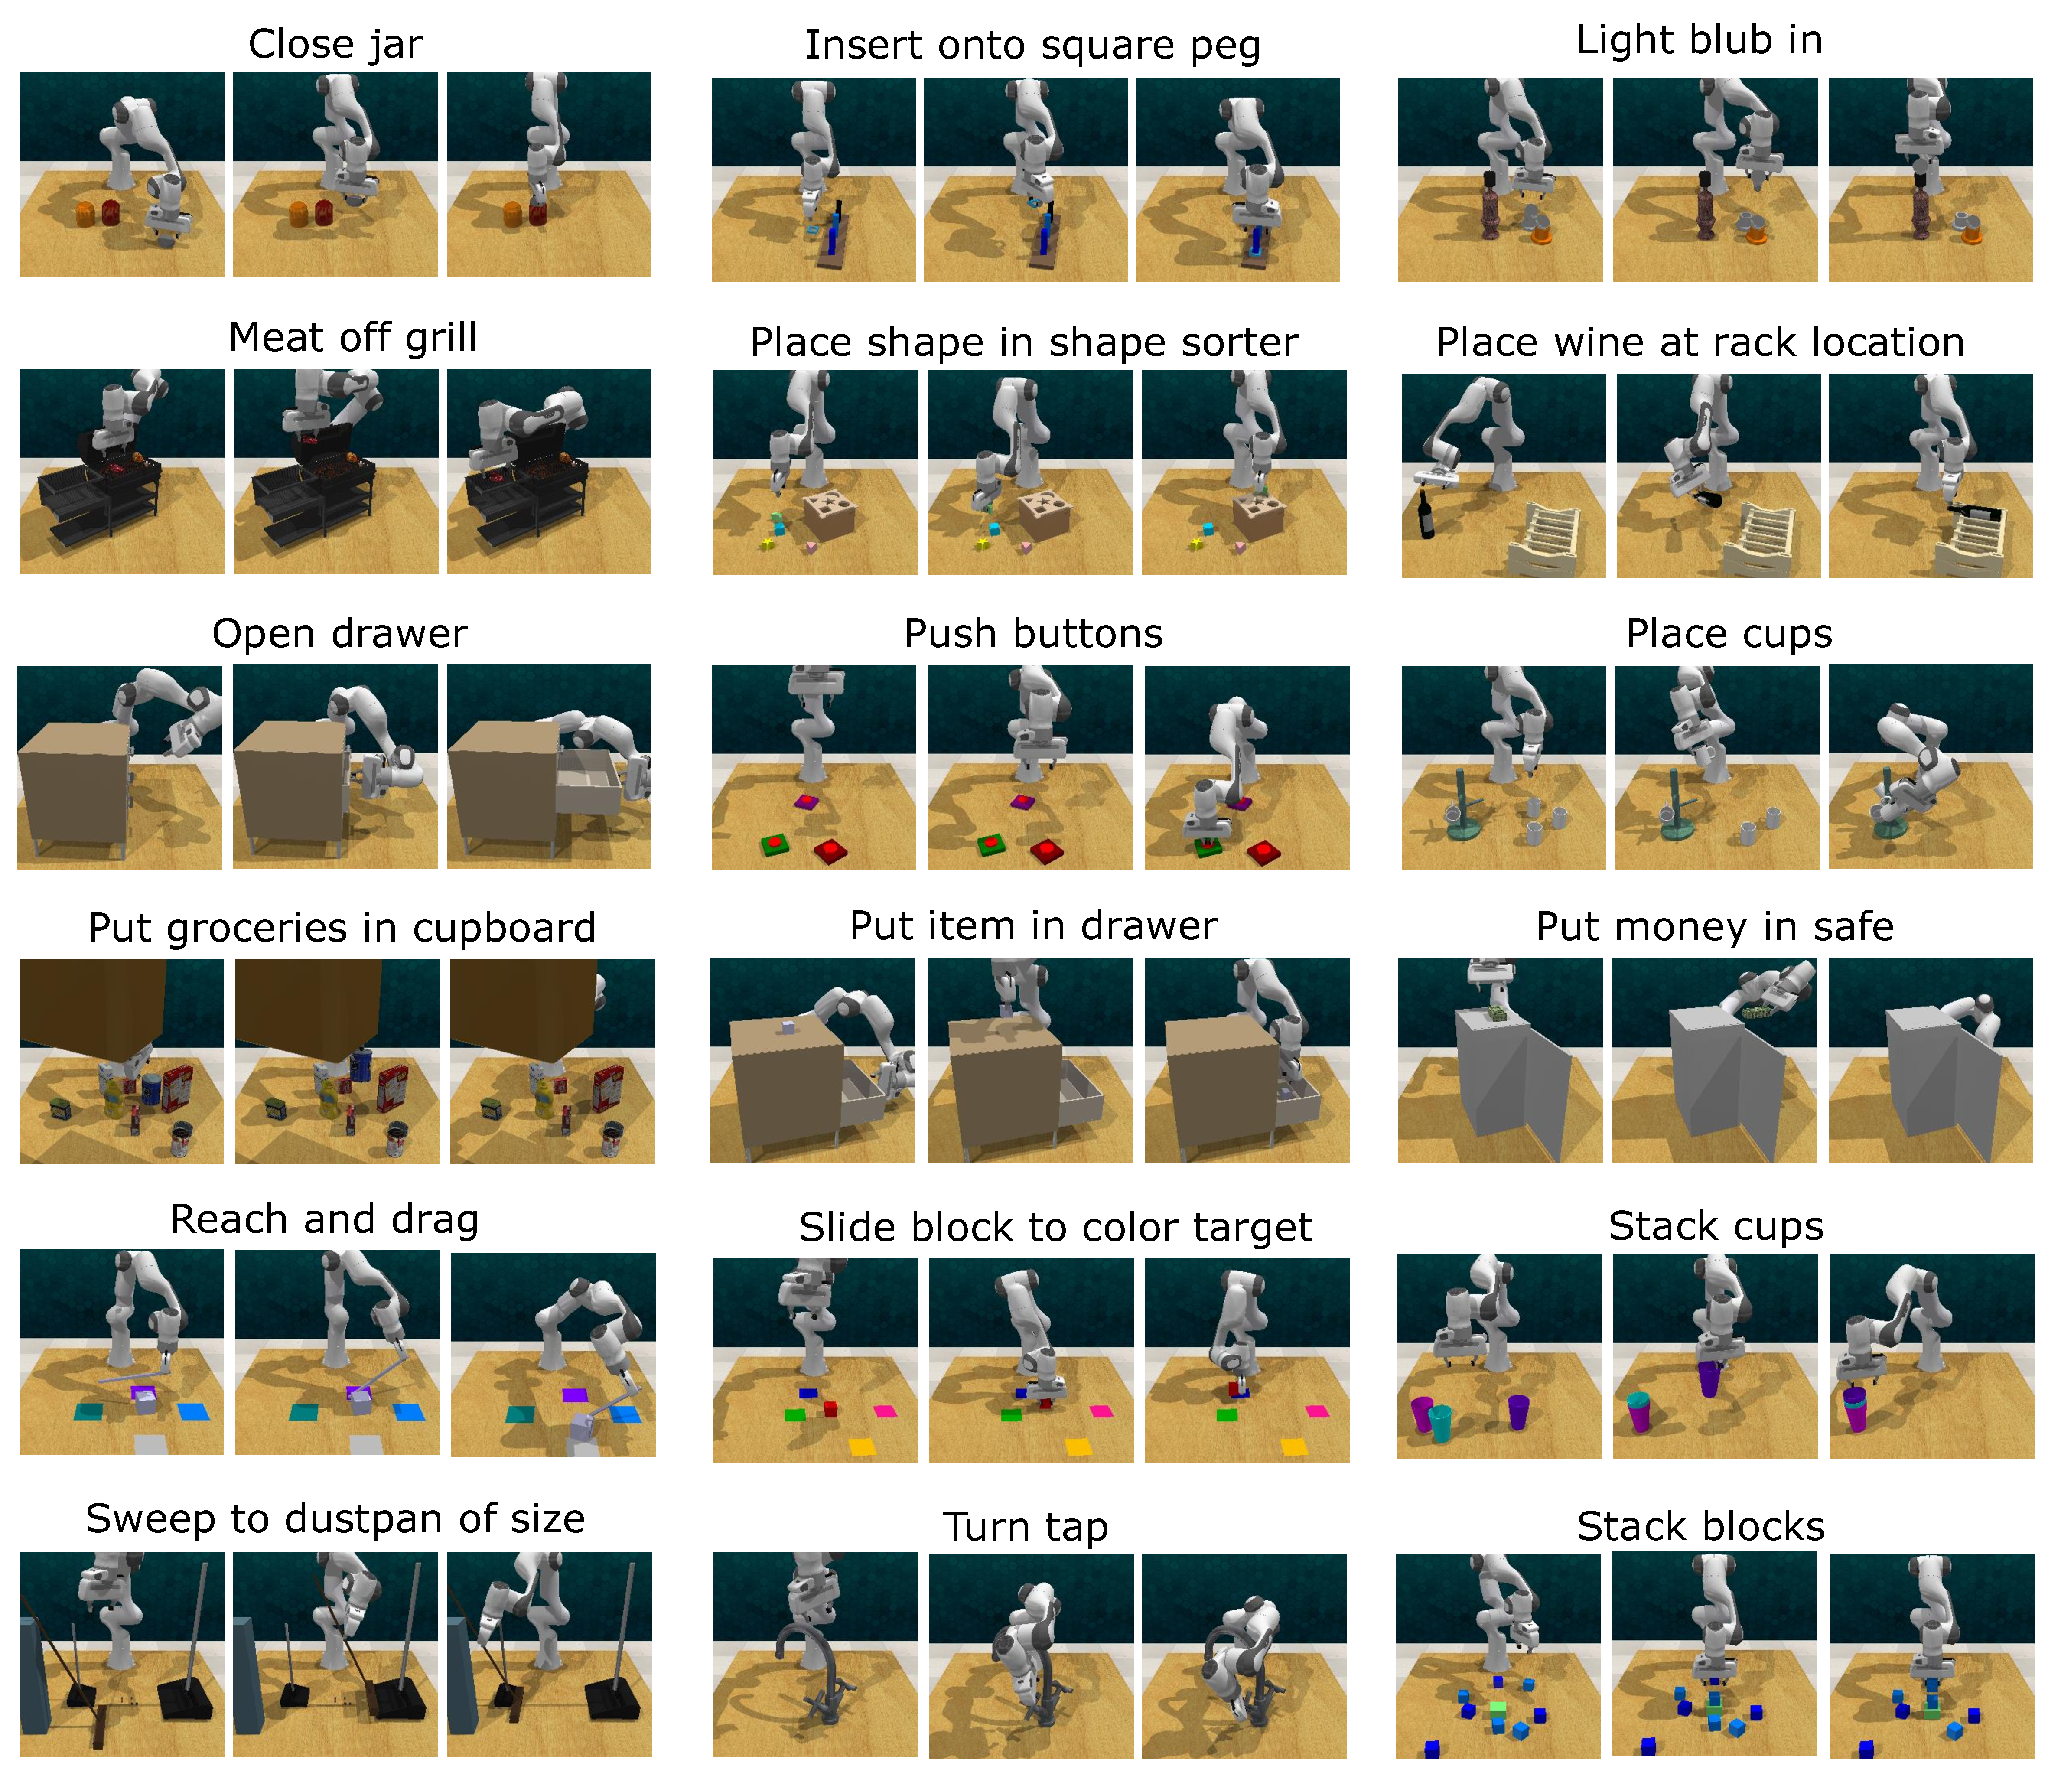
\includegraphics[width=0.92\textwidth]{figures/rlbench_task_grid.pdf}
  \caption{\textbf{The 18 RLBench Tasks.}
  Visualization of the 18 RLBench~\cite{james2020rlbench} tasks used in
  Sec.~\ref{sec:exp:rlbench}.}
  \label{fig:RLBench_VIS}
\end{figure*}

\begin{figure*}[t]
  \centering
  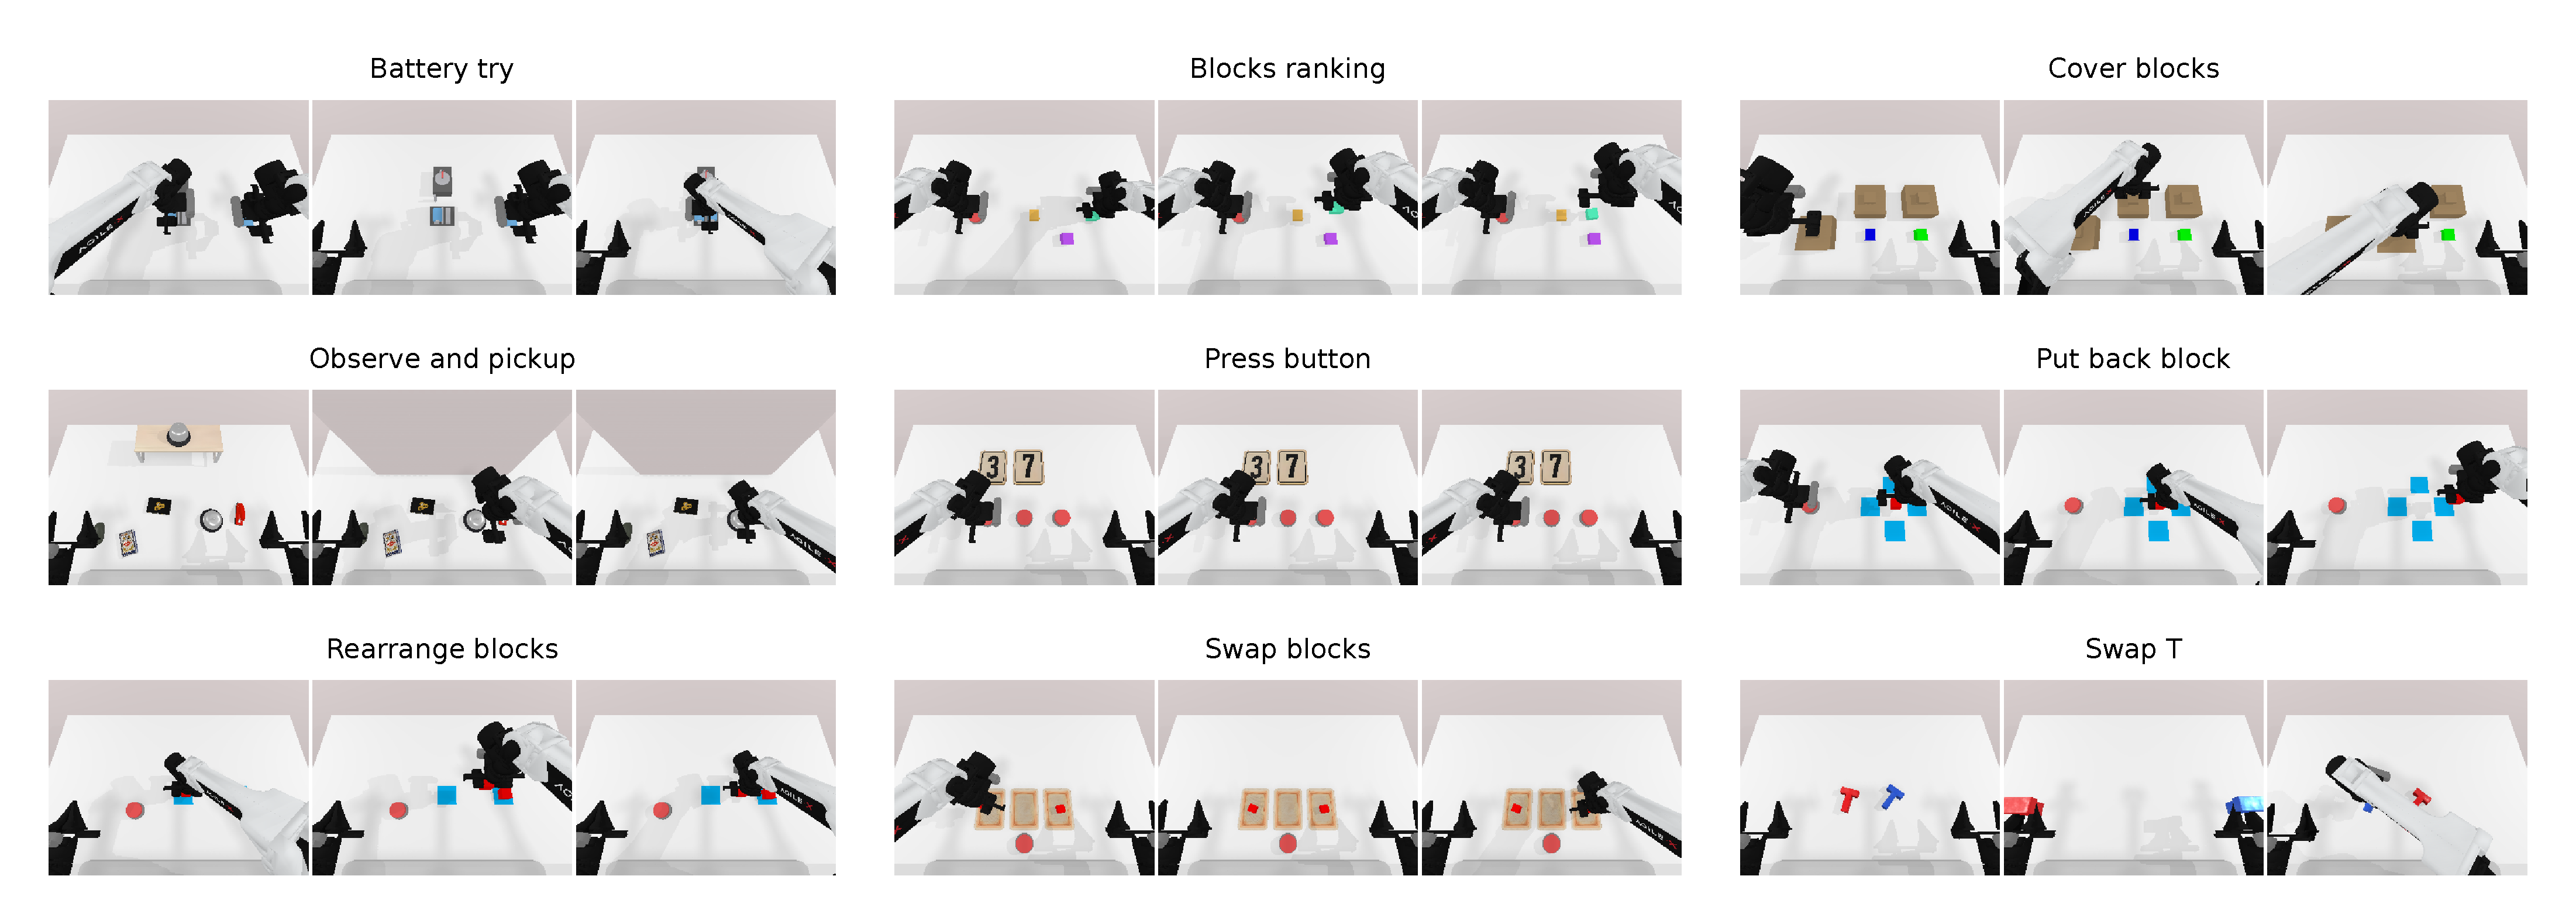
\includegraphics[width=\textwidth]{figures/rmbench_task_grid.pdf}
  \caption{\textbf{The Nine RMBench Tasks.}
  One evaluation rollout per task of RMBench~\cite{chen2026rmbench},
  shown as three frames in temporal order; the dual-arm tasks span the
  short-term $M(1)$ and long-term $M(n)$ memory regimes.}
  \label{fig:vis_rmbench}
\end{figure*}

% p13: COLOSSEUM perturbations (~620pt)
\begin{figure*}[t]
  \centering
  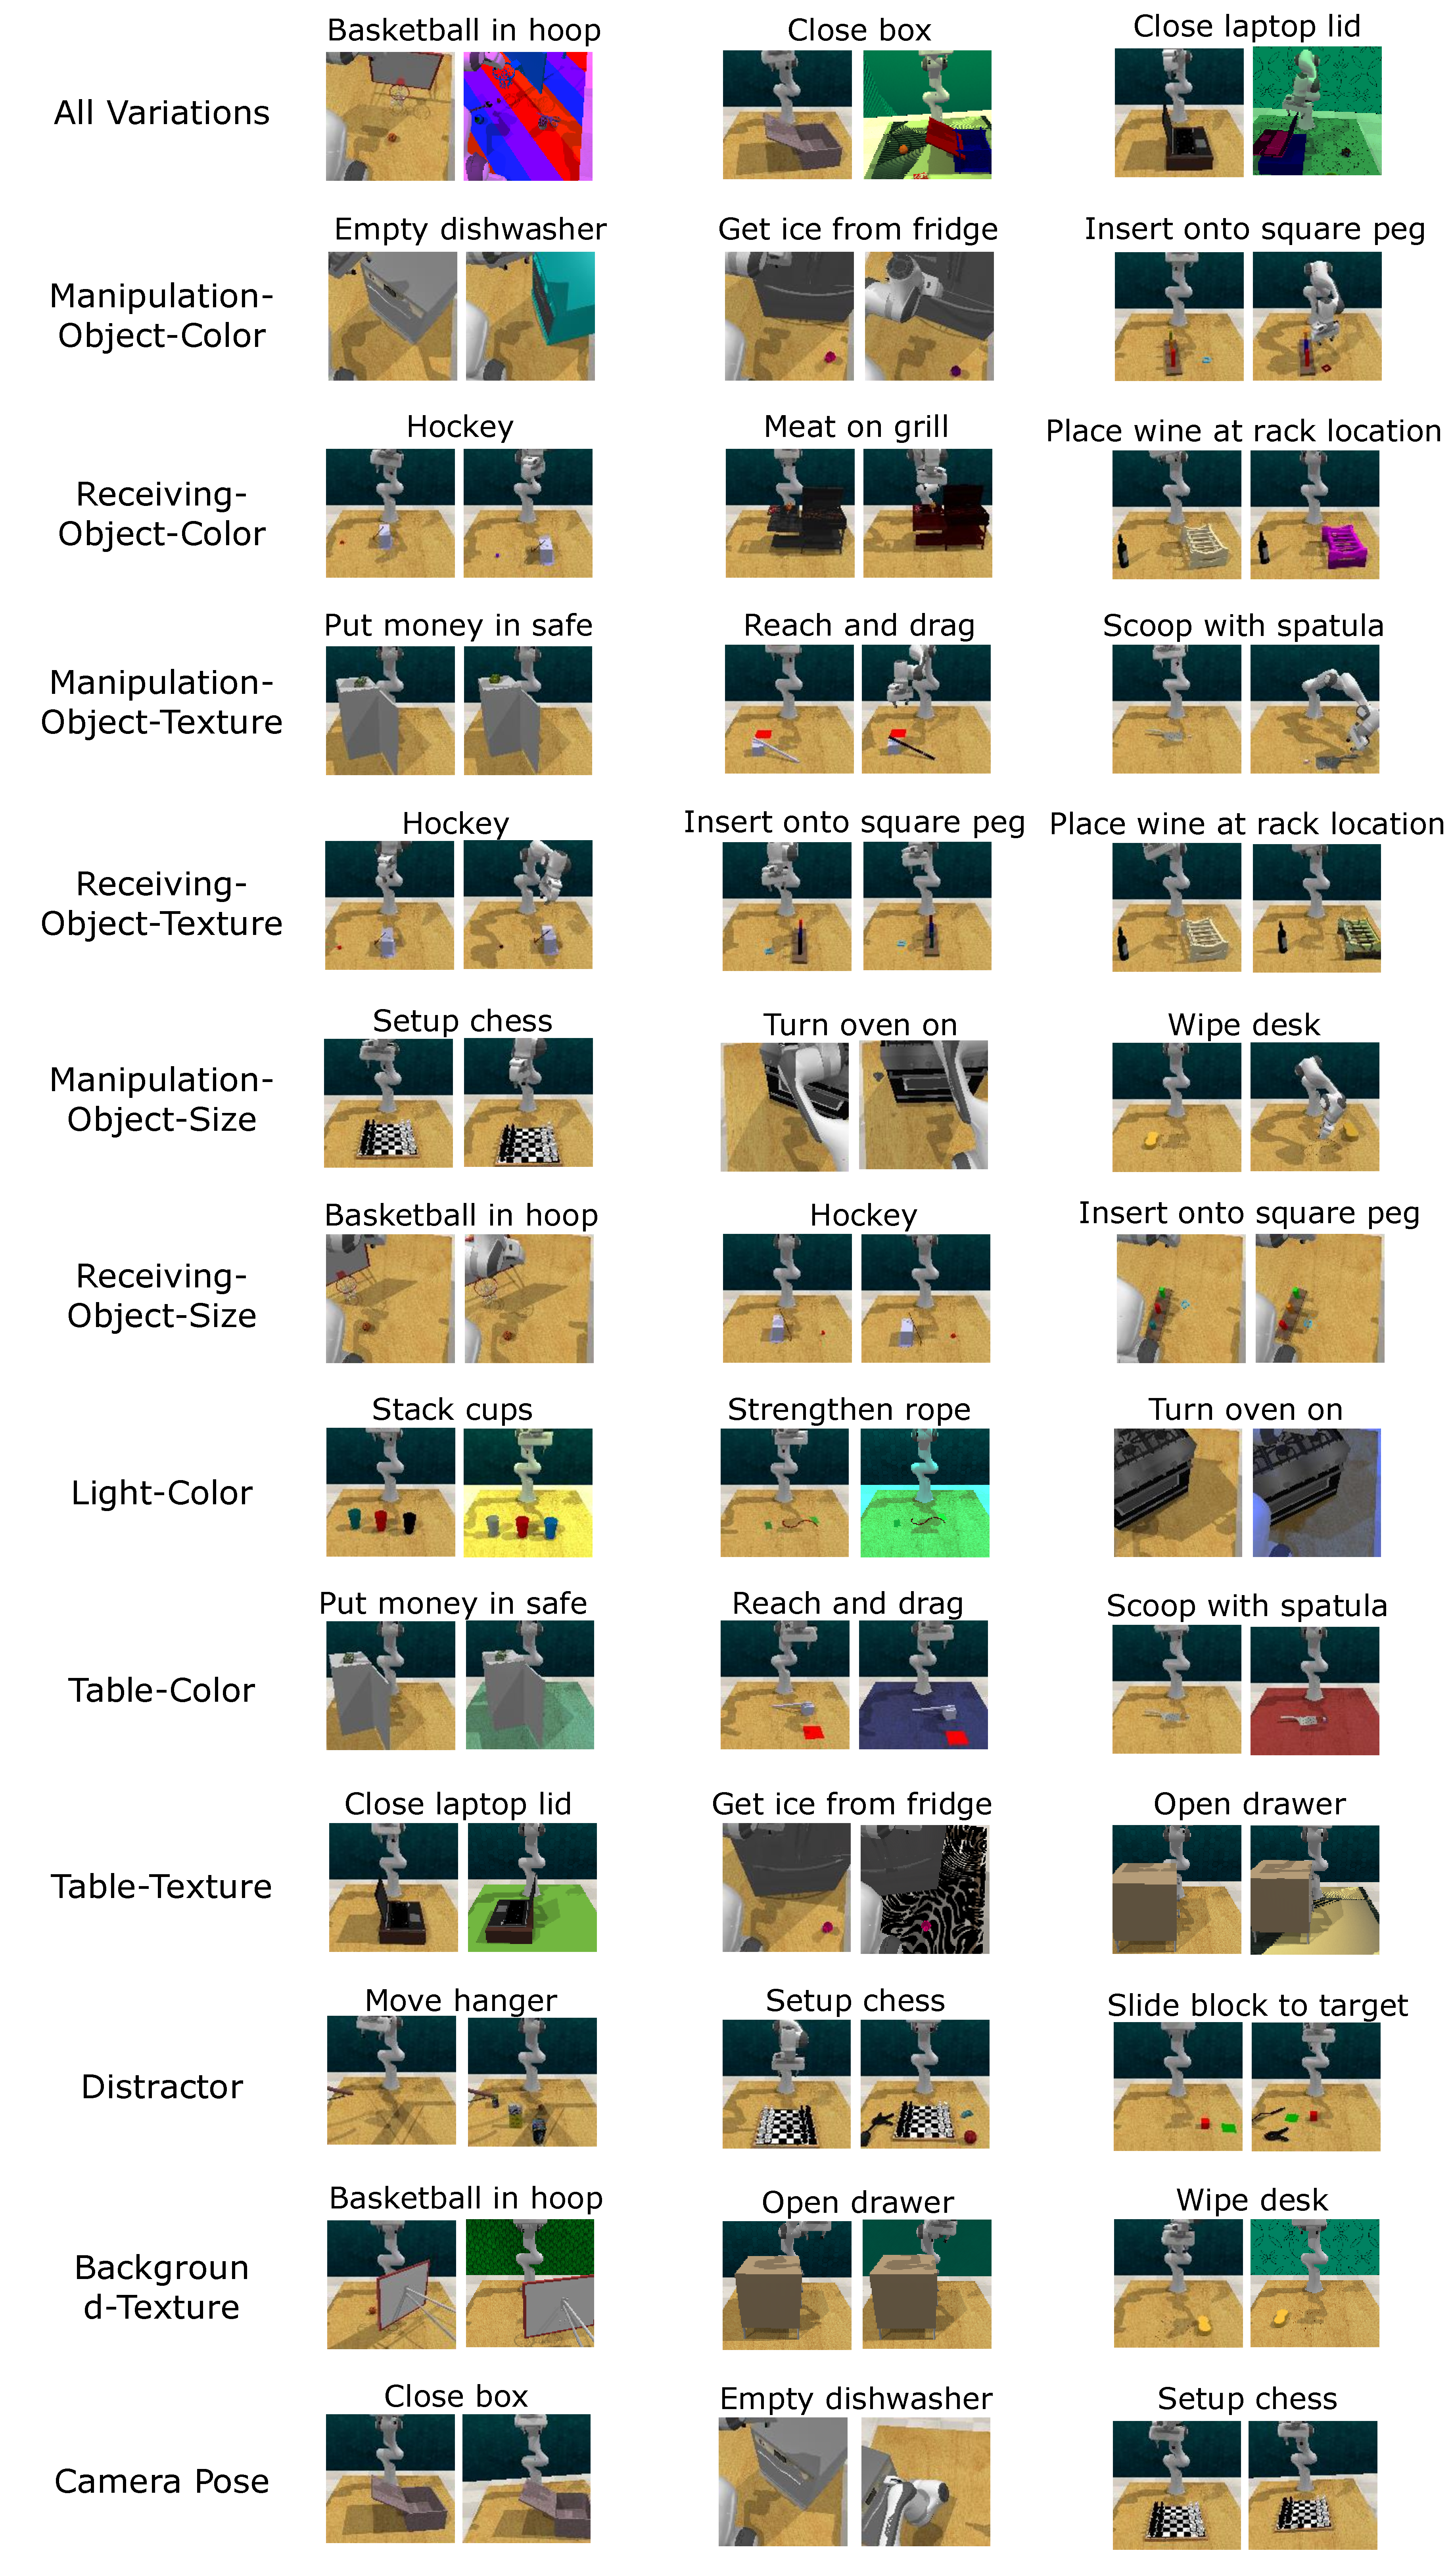
\includegraphics[width=0.7\textwidth]{figures/colosseum_perturbations.pdf}
  \caption{\textbf{Perturbations in COLOSSEUM~\cite{pumacay2024colosseum}.}
  All perturbation axes are shown except the original-RLBench variation
  setting.}
  \label{fig:vis_colosseum}
\end{figure*}

% p14: GemBench task grid (~415pt) + MemoryBench task grid (~205pt)
\begin{figure*}[t]
  \centering
  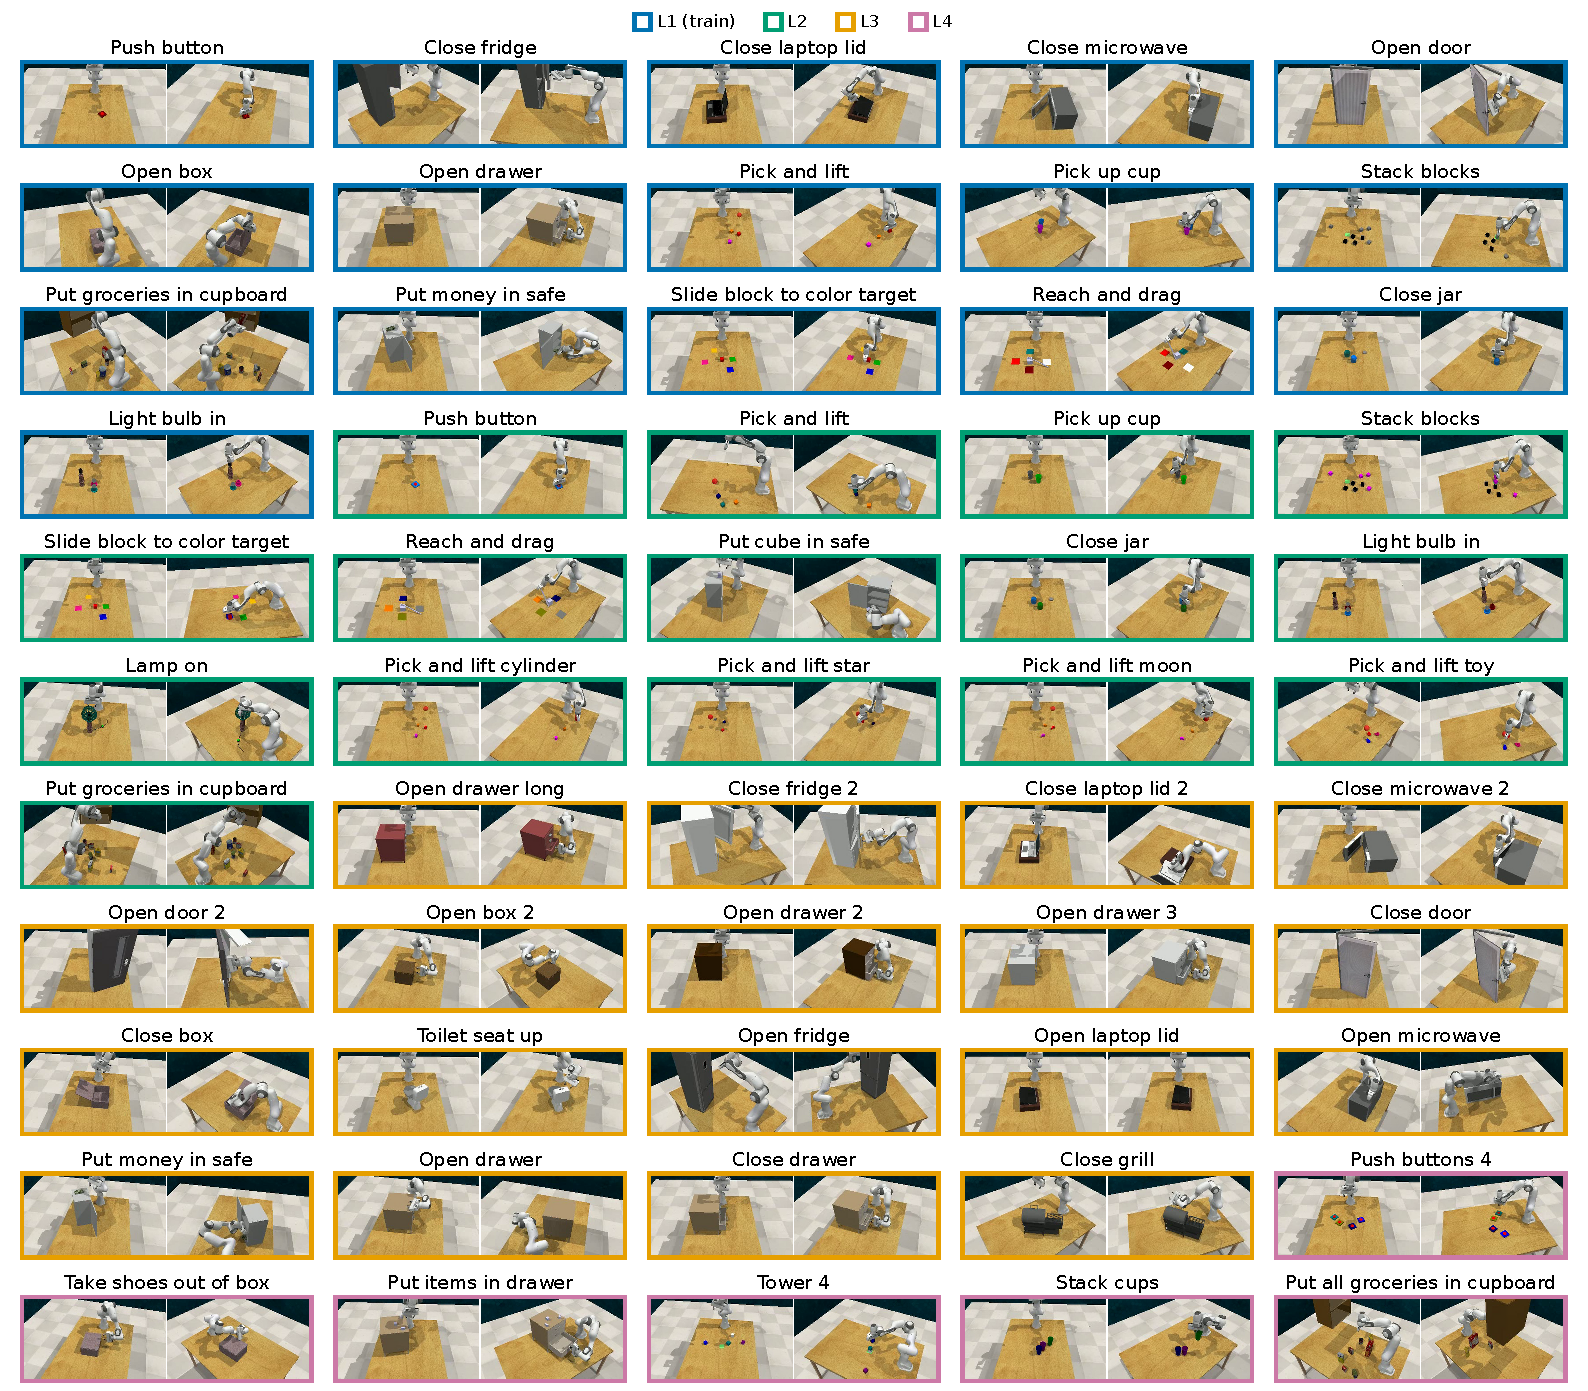
\includegraphics[width=0.88\textwidth]{figures/gembench_task_grid.pdf}
  \caption{\textbf{The GemBench Task Suite.}
  One representative variation of every task of
  GemBench~\cite{garcia2024towards}, shown as the first and final
  frame of an evaluation rollout.
  Border colors denote the generalization level: \emph{L1} (blue,
  novel placements), \emph{L2} (green, novel rigid objects), \emph{L3}
  (orange, novel articulated objects), and \emph{L4} (pink, novel
  long-horizon tasks).}
  \label{fig:vis_gembench}
\end{figure*}

\begin{figure*}[t]
  \centering
  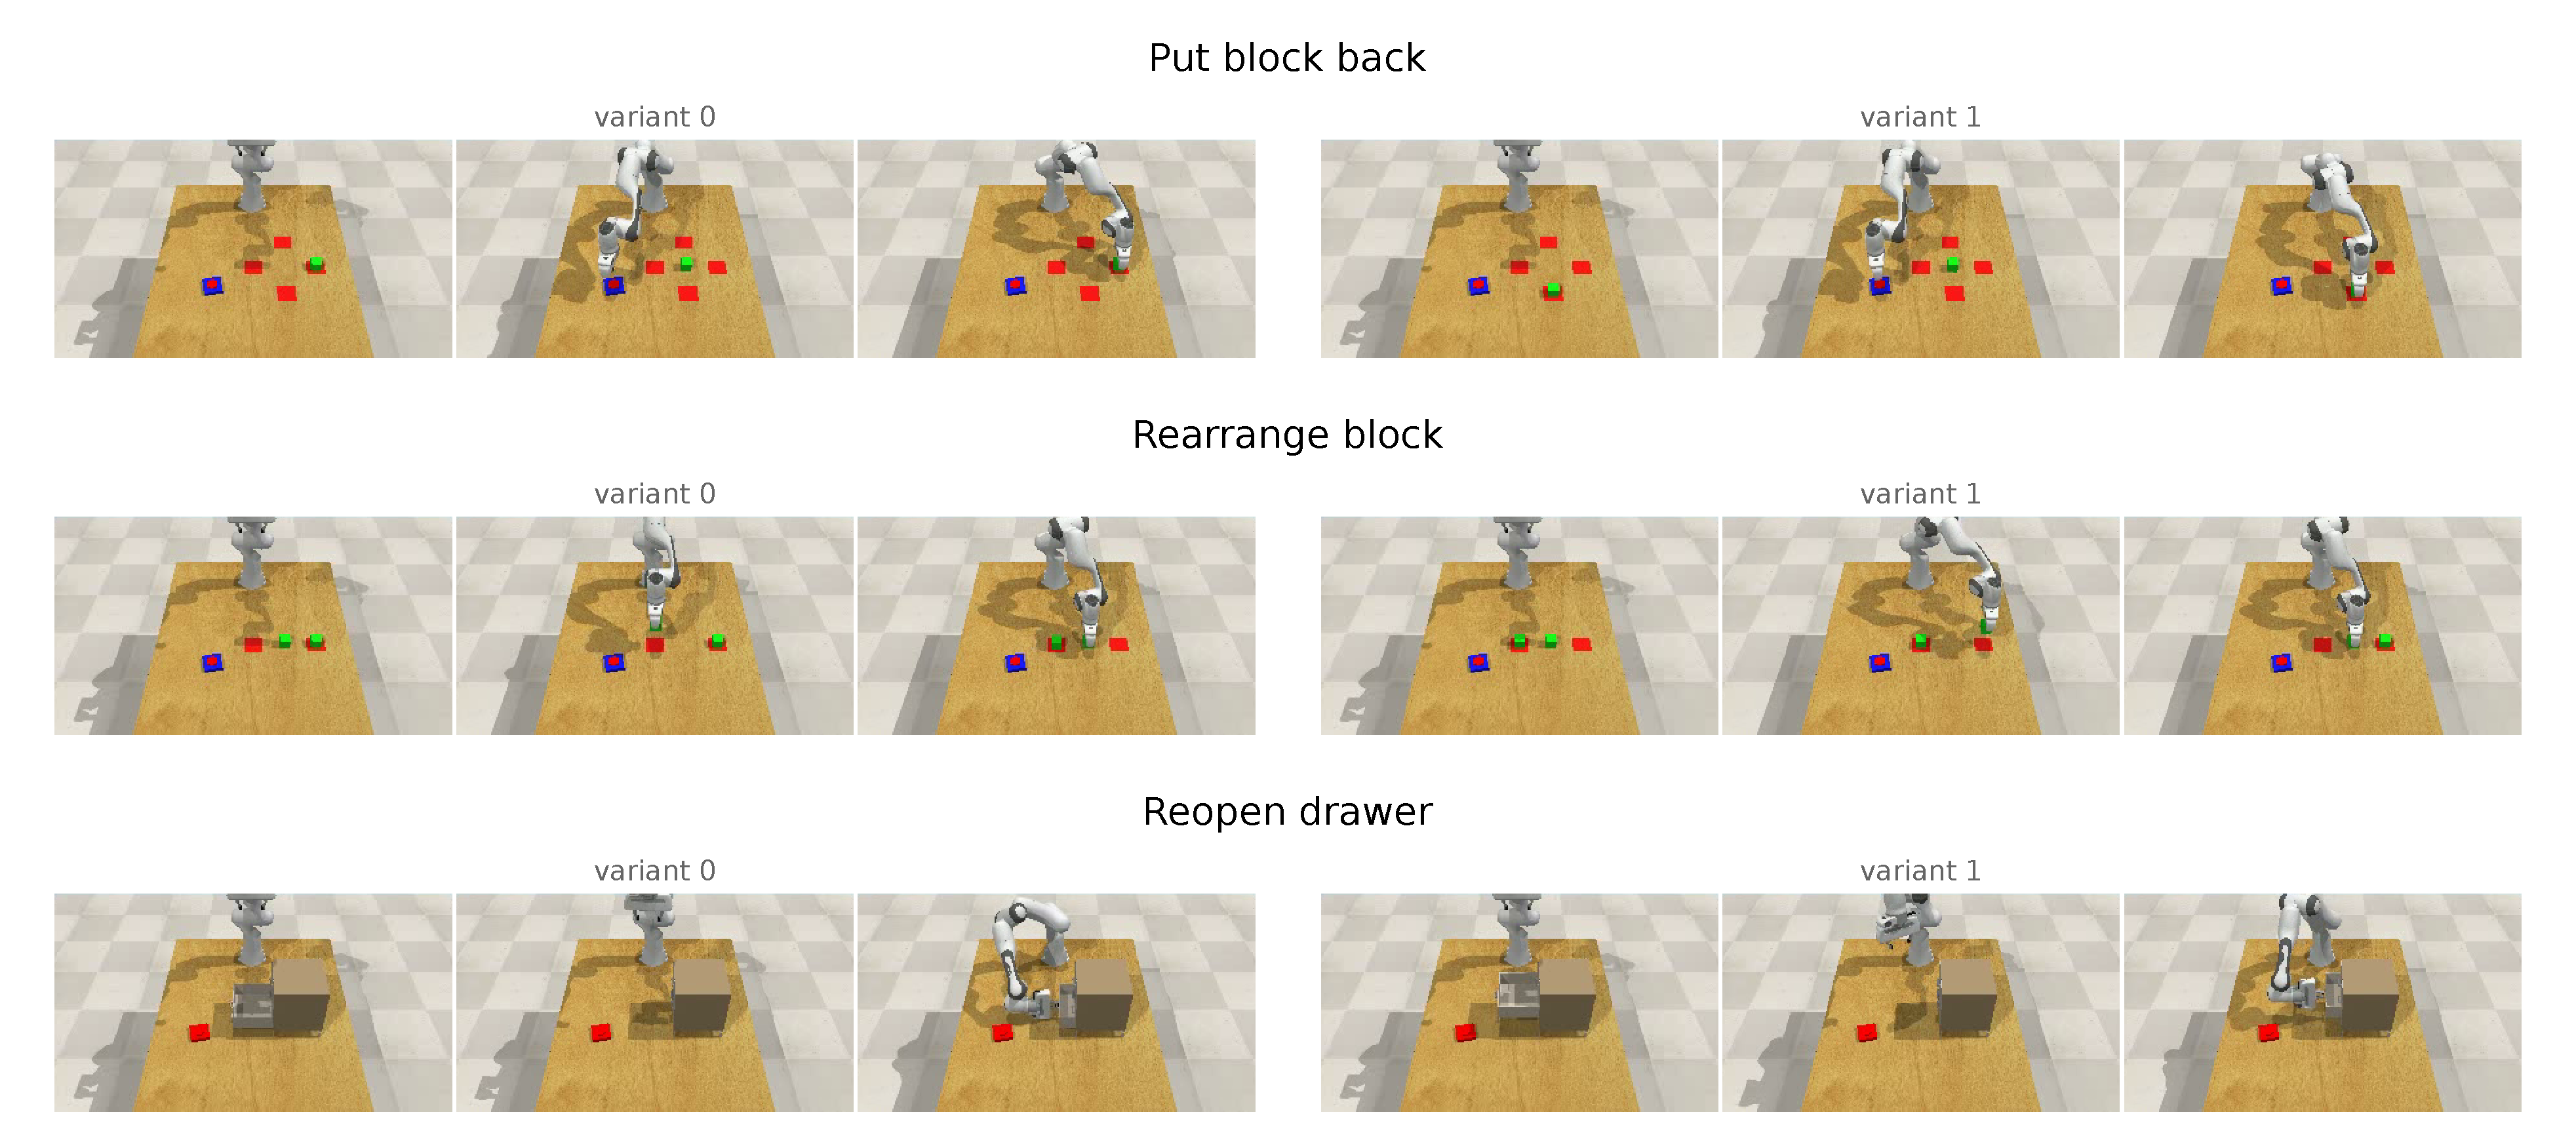
\includegraphics[width=0.8\textwidth]{figures/memorybench_task_grid.pdf}
  \caption{\textbf{The Three MemoryBench Tasks.}
  Two variants of each MemoryBench~\cite{fang2025sam2act} task, each
  shown as three rollout frames in which the robot's own intervention
  erases the evidence a later step depends on.}
  \label{fig:vis_memorybench}
\end{figure*}
